\documentclass[12pt, a4paper]{report}
%!TEX root = ../Report.tex
\usepackage[T1]{fontenc}
\usepackage[utf8]{inputenc}
\usepackage[english]{babel}
%slippery gypsy packages that need to come first, since others call them after
\usepackage[x11names,dvipsnames,svgnames,table]{xcolor}

% general incantations
\usepackage[export]{adjustbox}
\usepackage{afterpage}

\usepackage{graphicx}
\usepackage{placeins}
\usepackage{pdfpages}
\usepackage{algorithm2e}
\usepackage{array}
\usepackage{booktabs}
\usepackage[most]{tcolorbox}
\usepackage{calligra}
\usepackage{caption}
\usepackage{datetime}
\usepackage{dblfnote}
\usepackage{dirtytalk}
\usepackage{dsfont}
\usepackage{etex}
\usepackage{fancyhdr}
\usepackage{fix-cm}
\usepackage{textcomp,gensymb} %for \degree C symbol
\usepackage{graphicx}
\usepackage{lipsum}
\usepackage{listings}
\usepackage{transparent}
\usepackage[everyline=true,framemethod=tikz]{mdframed}
\usepackage{mparhack}
\usepackage{multicol}
\usepackage{multirow}
\usepackage{parskip}
\usepackage{lscape}
\usepackage{pdflscape}
\usepackage{pdfpages}
\usepackage{placeins}
\usepackage[document]{ragged2e}
\usepackage{rotating}
\usepackage{setspace}
\usepackage{subcaption}
\usepackage{threeparttable}
\usepackage{tabularx}
\usepackage[normalem]{ulem}
\usepackage{verbatim}
\usepackage{soul} %highlighting, strike through etc.


%Automated appendices
\usepackage[toc,titletoc,title,header]{appendix} %advanced functionality

%language settings

\usepackage{csquotes}

%page setup
%this where we adjust the binding offset, if relevant
\usepackage[a4paper,margin=2.54cm]{geometry}
\usepackage{lastpage} % for page 1 of n footers

%cross referencing
\usepackage[hidelinks]{hyperref}
\usepackage{cleveref}

%maths stuff
\usepackage{amsmath}
\usepackage{mathtools}

\setcounter{secnumdepth}{5}

%lists
\usepackage{enumitem}

%working collaboratively
\usepackage[backgroundcolor=yellow]{todonotes}

%reference list
\usepackage[backend=biber,style=ieee]{biblatex} %Sbliography with IEEE style.
\addbibresource{3_footer/ref.bib} %Imports bibliography file
\usepackage{url} %for URL fonts
\urlstyle{same}

%glossary for acronyms
\usepackage[acronym,nonumberlist,toc,section=subsection,numberedsection=nolabel]{glossaries}
\makeglossaries
\newacronym{abc}{ABC}{Australian Broadcasting Corporation}

%line spacing
\linespread{1.25}

% \newcommand{\subsubsubsection}[1]{\paragraph{#1}\mbox{}\\}
% \setcounter{secnumdepth}{4}
% \setcounter{tocdepth}{4}

\usepackage{caption}

\usepackage{listings}
  \definecolor{light-gray}{gray}{0.35}
	\lstdefinestyle{DOS}
	{
	    backgroundcolor=\color{light-gray},
	    basicstyle=\scriptsize\color{white}\ttfamily
	}
\usepackage{float}

\begin{document}

%!TEX root = ../Report.tex
\begin{titlepage}
\newgeometry{left=20mm,right=20mm,top=2.5cm,bottom=2cm}


\thispagestyle{empty}
\setlength\headheight{0pt}
\begin{center}

\begin{center}

\includegraphics[width=0.8\linewidth]{img/NUS_logo.jpg}
\end{center}

{\scshape\LARGE National University of Singapore \par}
\vspace{0.25cm}
{\scshape\Large cognitive systems project\par}
\vspace{0.5cm}

{\Large\bfseries IChat}

{\large\bfseries ISS Chatbot System}

\vspace{0.5cm}

\begin{minipage}{0.6\textwidth}
	\begin{flushleft} \large
    \emph{Group Members}\\
      LU JIAHAO\\
      ZHAO YAZHI\\
	\end{flushleft}
\end{minipage}~
\begin{minipage}{0.2\textwidth}
  \begin{flushright} \large
    \emph{Student ID}\\
    A0091835Y\\
    A0195305E\\
  \end{flushright}
\end{minipage}\\

\vspace{4cm}
Supervised by\par
FAN Zhen Zhen\\
NUS-ISS\par
\vspace{1.5cm}
\large
\today

\end{center}

\clearpage
\restoregeometry
\end{titlepage}
 % complete

\restoregeometry

\setcounter{tocdepth}{5}
\tableofcontents
% \clearpage

% \listoffigures
% \listoftables
% \pagebreak

%%%%%%%%%%%%%%%%%%%%%%%%%%%%%%%%%%%%%%%%%%%%%%%%%%%%%%%%%%%%%%%%%%%%%
% Executive Summary / Paper Abstract
% Sponsor Company Introduction (if applicable)
% Business Problem Background
% Project Objectives & Success Measurements
% Project Solution (To detail domain modelling & system design.)
% Project Implementation (To detail system development & testing approach.)
% Project Performance & Validation (To prove project objectives are met.)
% Project Conclusions: Findings & Recommendation

% List of Abbreviations (if applicable)
% References (if applicable)
%%%%%%%%%%%%%%%%%%%%%%%%%%%%%%%%%%%%%%%%%%%%%%%%%%%%%%%%%%%%%%%%%%%%%

\justify

\chapter*{Executive Summary}
%!TEX root = ../Report.tex
% Background
% General
Working in this ever-change world, No one can continue to grow only through past learning experiences. It is relieved that more and more people in Singapore are pursuing post-graduate studies \cite{postgrad}. Most of us decided on our Bachelor’s when we were young. Not all the people know what they want when taking a major. After gaining some experience during working, people have a clearer path and idea what they want.

% Mention NUS
National University of Singapore - Institute of Systems Science (NUS-ISS) upskills people through skills-based, industry-relevant courses so that they stay competitive in the digital age. The courses it provides is more practical and industry-based skills compared with traditional Postgraduate education \cite{nusiss}.

% What we may want
Although NUS-ISS has a user-friendly website, it may still be a challenge for a learner to find information fast and accurate. A research \cite{websiteuser} showed over 75\% users rank ease of finding the information as the most important factor in a website.

% What we can get from our product
For NUS-ISS website to successful, our team targets to create a chat bot. It can interact with user directly to answer relevant questions. The technology we utilised included Dialogflow \cite{dialogflow} and Slack \cite{slack}.
\clearpage

\chapter{Business Problem Background}
%!TEX root = ../Report.tex
NUS-ISS provides 3 categories of programmes. In each category, there are 4 to 12 different programmes. Over 130 courses are provided in these programmes.

With over 130 courses available in NUS-ISS website, how to efficiently answer the questions in the user's mind would be a challenge. For people who are not familiar with NUS-ISS website structure, it is difficult to get the information without trying clicking a lot of links.
\clearpage

\chapter{Objectives \& Success Measurements}
%!TEX root = ../Report.tex
\section{Objectives} % (fold)
\label{sec:objectives}
	The objective of this project is to create a chatbot system that will answer inquiries related to ISS programmes, courses and related information.

	The primary target audience of our system are people who are seeking advance knowledge and additional exposure to an area of interest from NUS-ISS. Our system will answer inquiries in an efficient way

% section objectives (end)

\section{Success Measurements} % (fold)
\label{sec:success_measurements}
	There are three key measures of our chatbot \cite{successmeasure}:
	\begin{enumerate}
		\item Whether the chatbot was able to understand the user
		\item Whether the chatbot was able to respond to the specific question being asked
		\item Whether the chatbot was able to present the related information
	\end{enumerate}

	% more detail would be added When Q&A is completed

% section success_measurements (end)
\clearpage

\chapter{Solution} % To detail domain modelling & system design
%!TEX root = ../Report.tex
\section{Assumptions} % (fold)
\label{sec:assumptions}

	\subsection{Target Audience} % (fold)
	\label{sub:target_audience}
	The major target audience would be the people pursuing post-graduate studies or professionals interested in practical and applicable skills in the industry.

	Current NUS-ISS students can also enjoy the benefit if they want to get the quick enquiry reply.
	% subsection target_audience (end)

	\subsection{Data Quality} % (fold)
	\label{sub:data_quality}
	All information used to build IChat is from NUS-ISS website \cite{nusiss}. It is assumed the data provided by NUS-ISS website are correct.
	% subsection data_quality (end)

% section assumptions (end)

\section{Project Scope} % (fold)
\label{sec:project_scope}
	In this project, a chatbot system (IChat) based on NUS-ISS website data is performed via Dialogflow \cite{dialogflow}. IChat focuses on two parts: \textbf{(i)} \textbf{intent-based system} \cite{intentsoverview}; \textbf{(ii)} \textbf{knowledge-based system} \cite{knowledgeconnector}. The inquires related to Graduate Programmes are replied by the former system while the inquiries related to the courses of Executive Education Programmes and Stackable Certificate Programmes are answered by the knowledge-based system.

	The intent-based system can answer question with context \cite{context} via \textbf{rich messages response} \cite{richmessage} option or manual input. It includes questions related to Admission \& Application, Career Path, Fee \& Loans, Modules, Overview and Project \& Internship for each Graduate Programme.

	The knowledge-based system can only answer questions for over 130 courses listed in Executive Education Flyer \cite{course}. It covers Course Overview, Key Takeaway, Target Audience, Prerequisites, Course Details, Fees \& Loans and Certification.
% section project_scope (end)

\section{Knowledge Model} % (fold)
\label{sec:knowledge_model}
	Knowledge modeling can be classified into three parts \cite{schreiber2001knowledge}:
	\begin{enumerate}[label=(\roman*)]
		\item Knowledge identification
		\item Knowledge specification
		\item Knowledge refinement
	\end{enumerate}

	\subsection{Knowledge Identification} % (fold)
	\label{sub:knowledge_identification}
		Knowledge identification sets the groundwork for the next stage encompassing knowledge specification. Information sources that are deemed to be useful are identified in preparation of knowledge acquisitions. In the context of building a chatbot, two main sources have been identified and are documented in Table \ref{table:knowledgesource}.

		\begin{table}[h]
		\centering
		\resizebox{\textwidth}{!}{%
		\begin{tabular}{|l|p{3cm}|p{5cm}|p{7cm}|}
		\hline
		\textbf{S/N} & \textbf{Source of Information} & \textbf{Insights from information sources} & \textbf{Knowledge acquisition technique} \\ \hline
		\textbf{1} & NUS ISS website & It provides basic information on different postgraduate programs & Data gathering from publicly available/documented information \\ \hline
		\textbf{2} & Generic Population & To validate and support the assumptions & Elicitation of tacit knowledge through analysis result of feedback from general population \\ \hline
		\end{tabular}%
		}
		\caption{Knowledge Source and Acquisition Technique}
		\label{table:knowledgesource}
		\end{table}
	% subsection knowledge_identification (end)

	\subsection{Knowledge Acquisition} % (fold)
	\label{sub:knowledge_acquisition}
		Following from the identification of knowledge sources, knowledge acquisition is conducted to capture the problem-solving domain knowledge. The techniques adopted to acquire the knowledge have been describe in Table \ref{table:knowledgesource} and the corresponding results are presented using a dependency diagram as shown in Figure \ref{fig:knowledge_model}.

		\begin{figure}[h]
			\centering
			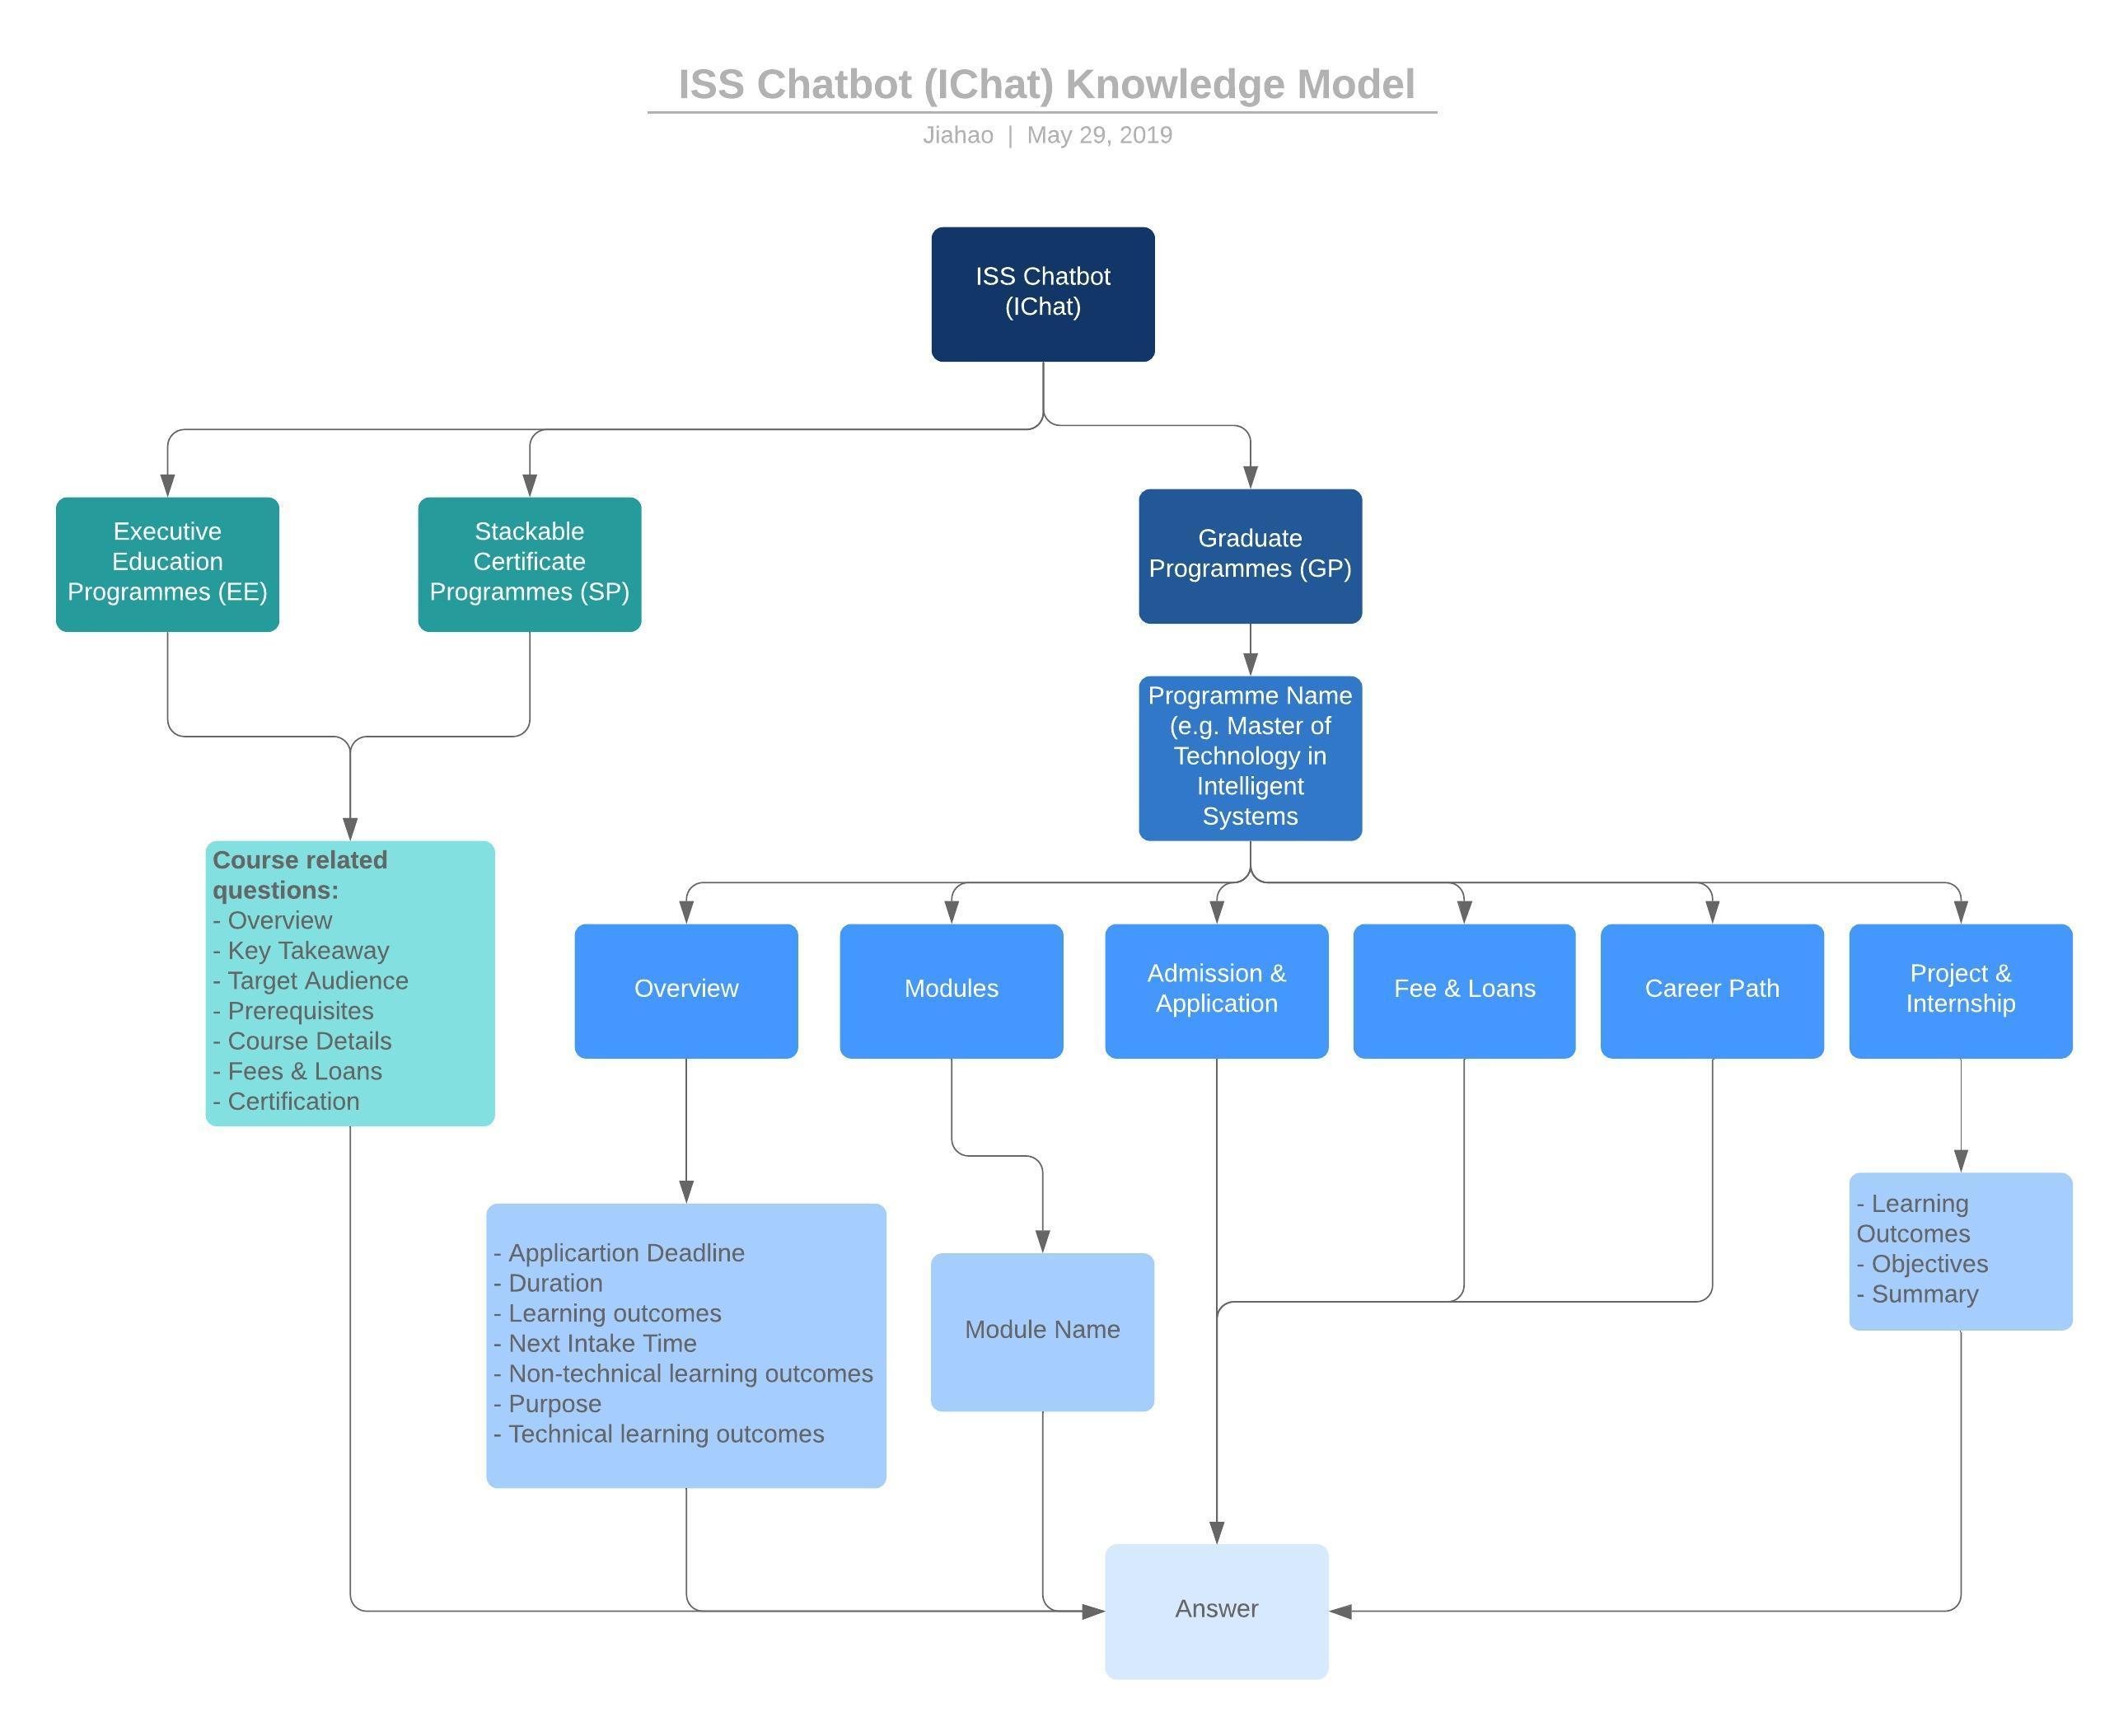
\includegraphics[width=\linewidth]{img/knowledge_model.jpeg}
			\caption{Domain Model of IChat}
			\label{fig:knowledge_model}
		\end{figure}

		The domain diagram arranges the factors affecting user’s question flow in a hierarchical tree structure. The top most level node represents the description of the proposed chatbot, which in this case, called iChat chatbot for NUS ISS website pages. This chatbot can be broken down into multiple layers of different components before arriving at the answers. These question flows are gathered from users of proposed question flow and represent their inherent preference. Table \ref{table:exampe_depedency} illustrates an example using the composition tree diagram in \ref{fig:knowledge_model}.

		The second level nodes represent the program we focused for the chatbot system and as well as the following detailed level nodes for more specific areas that may be asked within the chatbot system.

		\begin{table}[]
		\centering
		\resizebox{\textwidth}{!}{%
		\begin{tabular}{|l|p{4cm}|p{9cm}|}
			\hline
			S/N & \textbf{Category} & \textbf{Information} \\ \hline
			\textbf{1} & Observable & A user who is keen to explore postgraduate program in NUS-ISS \\ \hline
			\textbf{2} & Inferable sub-goals & The user in “1” might be interested in a master program. He/she might also be only eligible for a given subset of master program \\ \hline
			\textbf{3} & Top-level inference & The sub-goal in “2” is also one of the main factors that affects a user’s choice of a suitable master program \\ \hline
		\end{tabular}%
		}
		\caption{Example to Show A Part of the Dependency Diagram}
		\label{table:exampe_depedency}
		\end{table}
	% subsection knowledge_acquisition (end)

	\subsection{Knowledge Refinement} % (fold)
	\label{sub:knowledge_refinement}
		The knowledge refinement is an iterative process and it include model validation and model refinement. For model validation, different sets of test data will be used to run the simulation, and the result will be compared with sample data.

		For model refinement, after getting different actual results from expected results, we adjust the training phrases into different formats and retest it with the confidence score again to modify the model.
	% subsection knowledge_refinement (end)

% section knowledge_model (end)

\section{System Architecture} % (fold)
\label{sec:system_architecture}

	\begin{figure}[h]
		\centering
		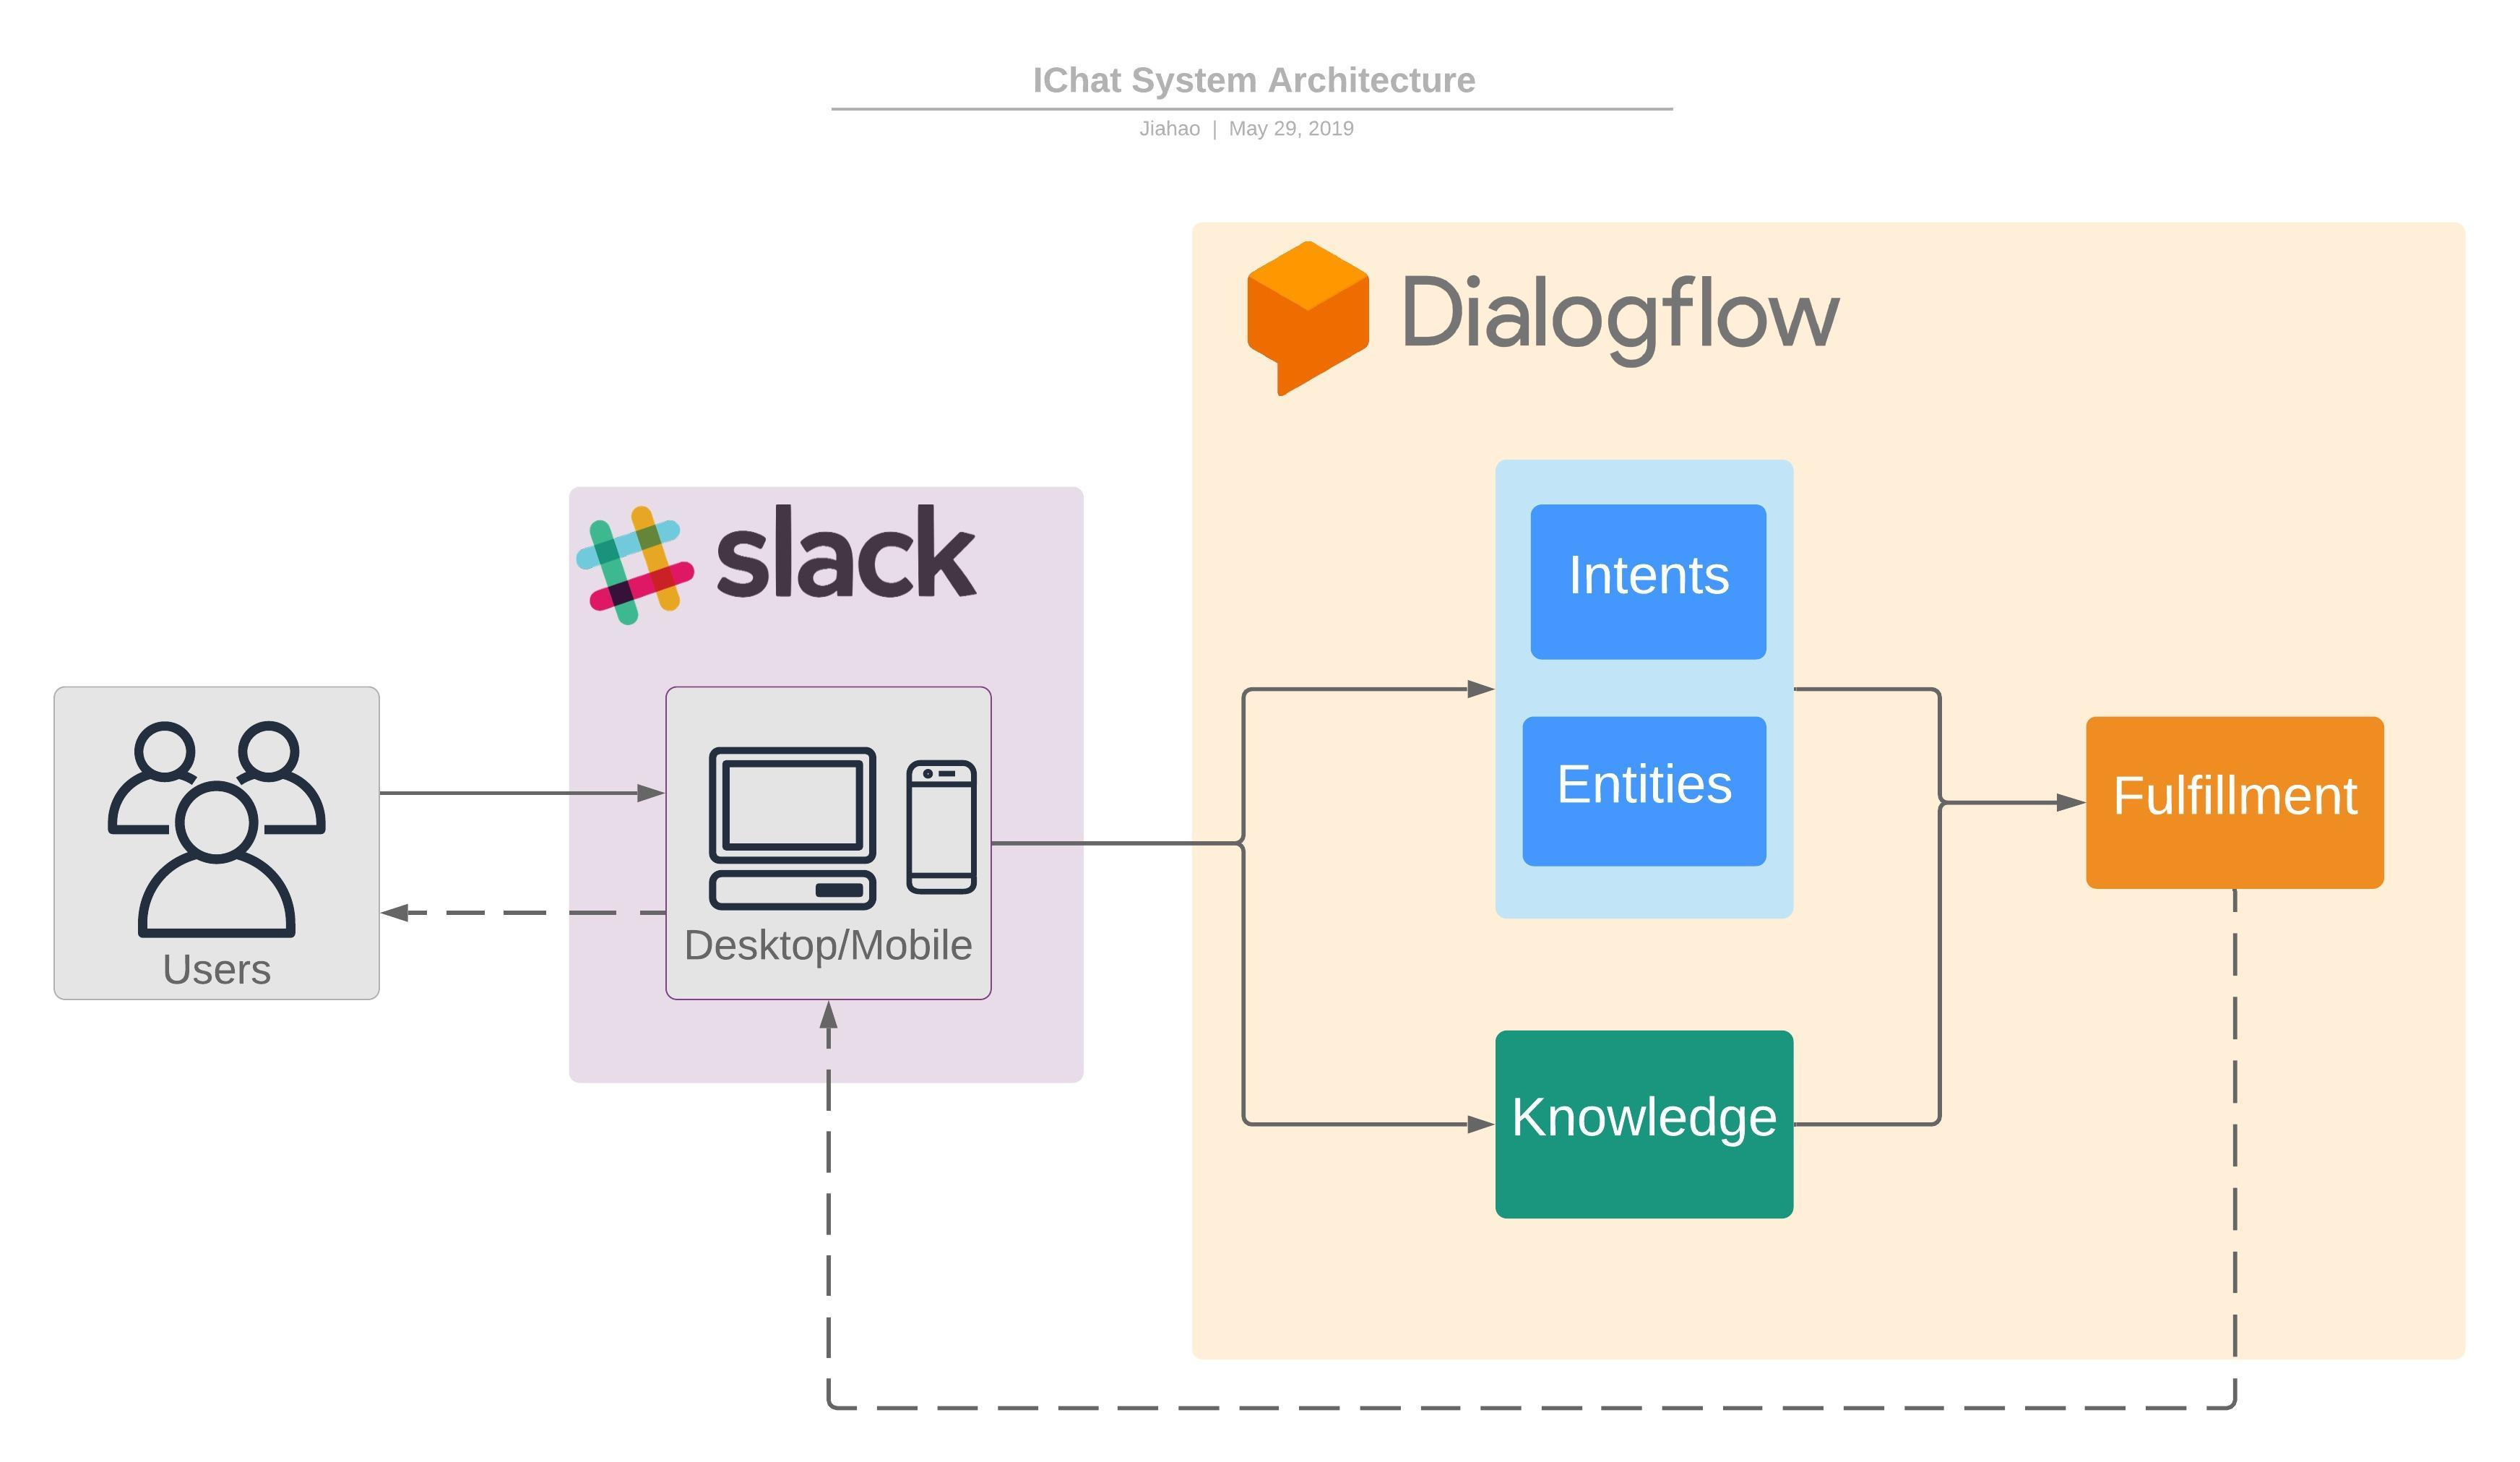
\includegraphics[width=\linewidth]{img/system_architecture.jpeg}
		\caption{System Architecture Diagram}
		\label{fig:system_architecture_diagram}
	\end{figure}
	Figure \ref{fig:system_architecture_diagram} shows the system architecture diagram of IChat. It illustrates how the different components interact with each other through Dialogflow. After the user keys in the inputs in the Slack by either mobile phone or computer, Slack will be passed the input through the Dialogflow to process. Based on the enquiries from the user, Dialogflow will choose either intent-based system or knowledge-based system to answer. Then the data will be passed to fulfillment and return the results to Slack so the user can read the answer.
% section system_architecture (end)
\clearpage

\chapter{Implementation} % To detail system development & testing approach.
%!TEX root = ../Report.tex
\section{Dialogflow Set-up} % (fold)
\label{sec:dialogflow_setup}
	In IChat, the beta feature ``Knowledge Bases'' is used. So we need to enable it before building the knowledge.

	To simplify the deployment, we use Inline Editor \cite{webhook} (Powered by Cloud Functions for Firebase). It would match a user's query to make suggestions or reply an answer.

	The details would be illustrate in Appendix \ref{cha:user_s_manual} (User's Manual).
% section dialogflow_setup (end)

\section{FAQ Knowledge Test} % (fold)
\label{sec:faq_knowledge_test}
	For Executive Education programs and Stackable Certificate Programs under NUS-ISS website, our team crawled the content from the web page as the knowledge document to build a FAQ document in Dialogflow. However, one question can be phrased into many different ways. If the certain key word are replaced or missing from the question, IChat won’t be able to provide a correct answer. For example, ‘cost’ are trained as the key word for question related to school fees or loans inside the knowledge document. But when user enter word like ‘how much’ or ‘price’, IChat cannot provide the answer related to school fees. Therefore, our team decides to do a knowledge document validation.

	Knowledge document validation is an iterative process and our team focuses on question refinement. For question refinement, different sets of test data is used to run the simulation, and result will be compared with previous iteration to get the highest accuracy rate. Full knowledge document validation question, together with the result are listed in Table \ref{table:faq_test} of Appendix \ref{cha:test_result}.

% section faq_knowledge_test (end)

\section{Intent Test} % (fold)
\label{sec:intent_test}
	For Graduate Programs under NUS-ISS website, our team decide to use intent and fulfillment to represent knowledge to related questions.

	Intent validation is conducted based on the intent we created and training sets we provided in the fulfillment. Different sets of test data is used to run the simulation. Intent details, together with the testing result are appended in Table \ref{table:intent_test} of Appendix \ref{cha:test_result}.
% section intent_test (end)

\section{UI Test} % (fold)
\label{sec:ui_test}
	To get a good user experience, we tested different integration tools \cite{integrations} provided in Dialogflow. The test includes \textbf{Web Demo}, \textbf{Facebook Messenger} and \textbf{Slack}.

	\subsection{Web Demo} % (fold)
	\label{sub:web_demo}
		In the beginning, we wanted to add Web Demo into NUS-ISS website. It successfully replied the user when we said ``hi'' (Figure \ref{fig:web_demo_reply_1}). However, after we had more tests, we realized Web Demo can not reply more than one message and cannot correctly pop up the suggestions we set up in the fulfillment. It only gave the last message showed in Figure \ref{fig:web_demo_reply_2}.

		\begin{figure}[h]
			\centering
			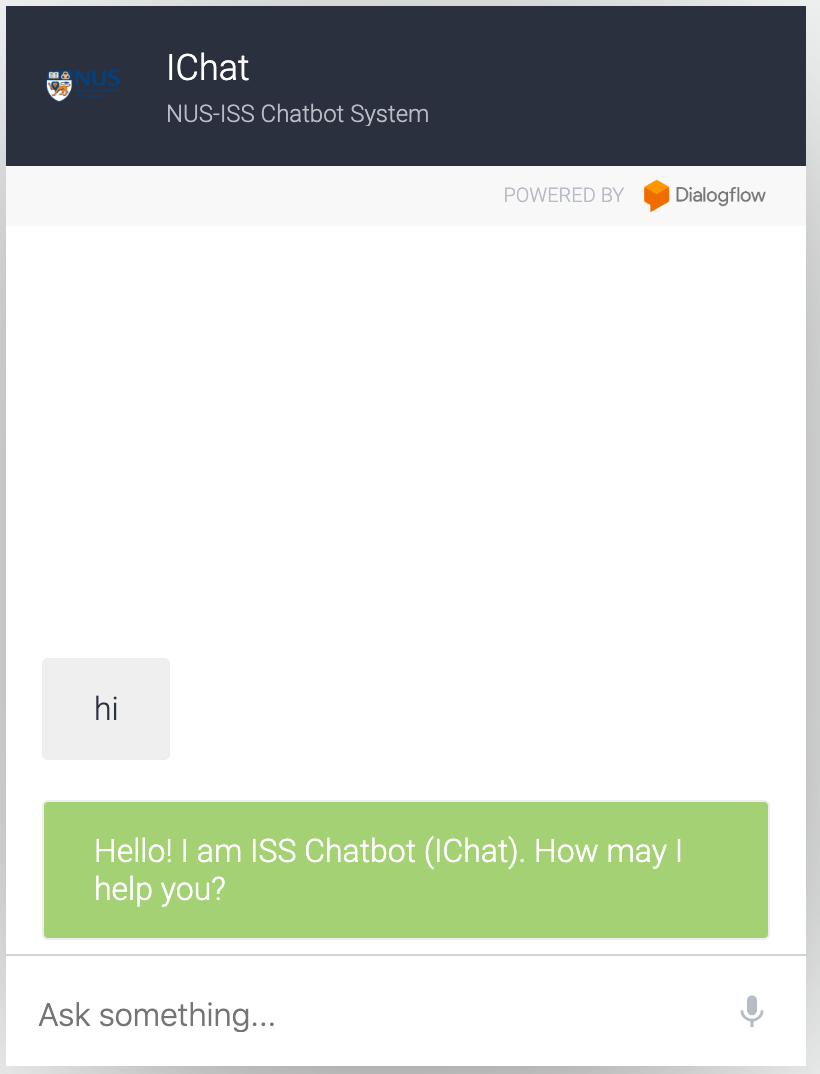
\includegraphics[width=\linewidth/3]{img/webdemo_1.png}
			\caption{Web Demo Reply 1}
			\label{fig:web_demo_reply_1}
		\end{figure}

		\begin{figure}[h]
			\centering
			
\includegraphics[width=\linewidth/3]{img/webdemo_2.png}
			\caption{Web Demo Reply 2}
			\label{fig:web_demo_reply_2}
		\end{figure}
	% subsection web_demo (end)

	\subsection{Facebook Messenger} % (fold)
	\label{sub:facebook_messenger}
		The Facebook Messenger successfully gave suggestions (Figure \ref{fig:fb_reply_1}) but with one line suggestion which was not very friendly to click if several suggestions were provided. Furthermore, when we clicked the follow-up suggestions, it would cancel the suggestion buttons if the suggestion was not the last message (Figure \ref{fig:fb_reply_2}).

		\begin{figure}[h]
			\centering
			
\includegraphics[width=\linewidth/3, frame]{img/fb_1.png}
			\caption{Facebook Messenger Reply 1}
			\label{fig:fb_reply_1}
		\end{figure}

		\begin{figure}[h]
			\centering
			
\includegraphics[width=\linewidth/3, frame]{img/fb_2.png}
			\caption{Facebook Messenger Reply 2}
			\label{fig:fb_reply_2}
		\end{figure}
	% subsection facebook_messenger (end)

	\subsection{Slack} % (fold)
	\label{sub:slack}
		At last, we chose Slack which can give a relatively good result (Figure \ref{fig:slack_reply_1}) compared with Web Demo and Facebook Messenger. It gave suggestions and still kept them in the history (Figure \ref{fig:slack_reply_2}) so the user are more flexible to go back choosing other questions. Since Slack can be accessed from different devices, it means the user can enquiry via mobile or desktop.

		\begin{figure}[h]
			\centering
			
\includegraphics[width=\linewidth/2, frame]{img/slack_1.png}
			\caption{Slack Reply 1}
			\label{fig:slack_reply_1}
		\end{figure}

		\begin{figure}[h]
			\centering
			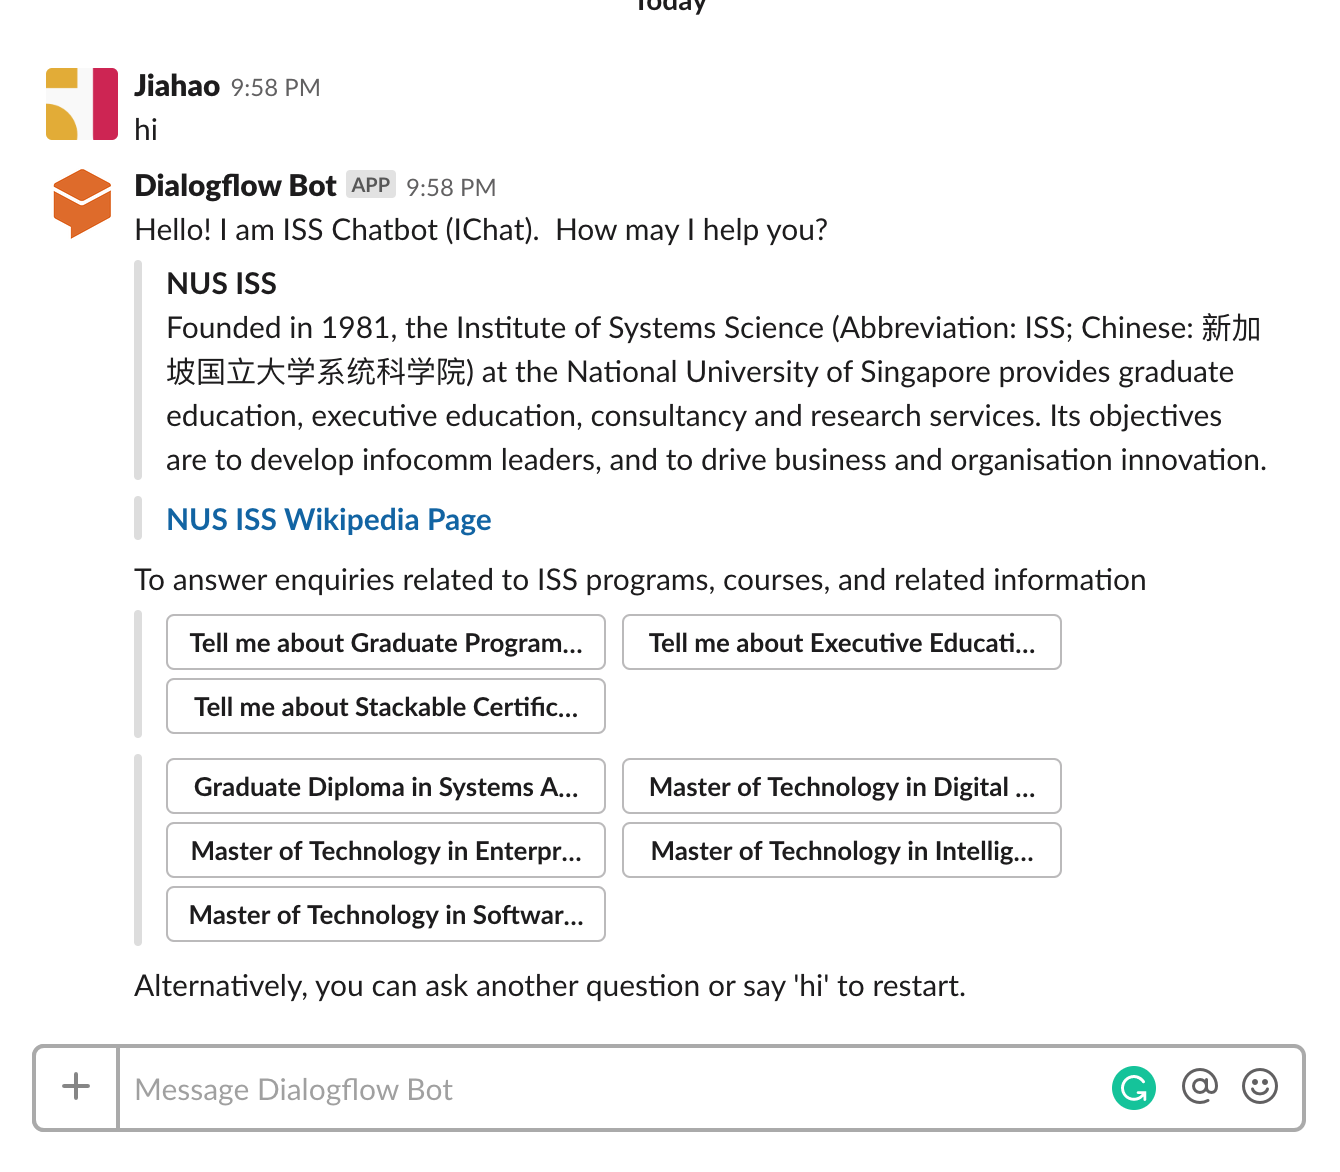
\includegraphics[width=\linewidth/2, frame]{img/slack_2.png}
			\caption{Slack Reply 2}
			\label{fig:slack_reply_2}
		\end{figure}
	% subsection slack (end)

% section ui_test (end)
\clearpage

\chapter{Performance \& Validation} % To prove project objectives are met.
%!TEX root = ../Report.tex
We perform validation on 2 different scenarios (shown in Appendix \ref{cha:demo}) to ensure that IChat provides the correct expected output.

Scenario 1 is a future student wants to check some information about \textbf{Master of Technology in Intelligent Systems}, which is under \textbf{Graduate Programme}. This student wants to know when the next intake time and how long will the programme last. In this scenario, the user only need to click suggestion button to get answers.

Scenario 2 is an employee wants to learn more about \textbf{Machine Reasoning} course in \textbf{Executive Education Programmes}. The user needs to input questions related to the course in this scenario.

According to Success Measurements mentioned in Section \ref{sec:success_measurements}, IChat proved its performance in these scenarios.
\clearpage

\chapter{Conclusions} % Findings & Recommendation
%!TEX root = ../Report.tex

Our project, IChat, is a chatbot coginitive system that will generate related answer for user requests about NUS-ISS programmes, courses and related information.
By using IChat, user can easily get useful and related information from different programmes provided by NUS-ISS.


\section{Improvements} % (fold)
\label{sub:improvements}

With the limited time, our project scope was diminished to a minimum viable product (MVP) level, which is version 1.0. Here is the full scope for the commercial version:

\begin{description}[align=left]
	\item [version 1.1] Include More Data

		To get better result, an advanced method should be used to scrape the data. Add more data fields like lecturers and their detail information for a specific course should be included for a better reply.

	\item [version 1.2] Add API

		An API should be created to fetch dynamic data instead of coding in "Inline Editor" of Dialogflow.

	\item [version 1.3] User Interface

		Although Slack can provide an acceptable user interface, there are still some limit like button length and numbers. Message Menus \cite{messagemenu} could be an option. Even so, for the moment a user needs to use Slack to inquire. Integrating a chatbot like kommunicate \cite{kommunicate}with the NUS-ISS website would help user get a much smoother experience.

	% \item [version 0.5] Fuzzy Logic Improvement

	% 	For miles cards and rewards cards, the current version 0.1 only includes a basic fuzzy logic is used to estimate the cash value of miles and rewards points. To get a better result, detailed data on miles and rewards points conversion are required to match a better cash value.

\end{description}
% section improvements (end)


% \section{Limitations} % (fold)
% \label{sub:limitations}

% As \href{https://www.moneysmart.sg/credit-cards}{MoneySmart} only covers most popular credit cards in Singapore, some credit cards may not be included for the recommendation.

% To simplify the calculation, only long term major features of the cards were included. Some would be manually converted to cash value for comparison.

% As there are some special credit cards for specific groups of people, these cards are excluded in the system. The system also excludes all special term for special employee benefits.

% section limitations (end)
\clearpage


\chapter{References}
\label{cha:ref}
\printbibliography[heading=none]

\clearpage

\begin{appendices}
  %!TEX root = ../Report.tex

% User Manual
\chapter{User's Manual} % (fold)
\label{cha:user_s_manual}

\section{Prerequisite} % (fold)
\label{sec:prerequisite}
To use Dialogflow and Slack, the following account is required:
\begin{itemize}
	\item Gmail Account
	\item Slack Account
\end{itemize}
If you do not have these two accounts, please go to Slack (https://slack.com/signin) or Google (https://accounts.google.com/sigNup) to register.

\clearpage
% section prerequisite (end)


\section{Import Agent} % (fold)
\label{sec:import_agent}

\begin{enumerate}

	\item Go to Dialogflow Console (https://console.dialogflow.com), then click “Create new agent”

	\begin{figure}[H]
		\centering
		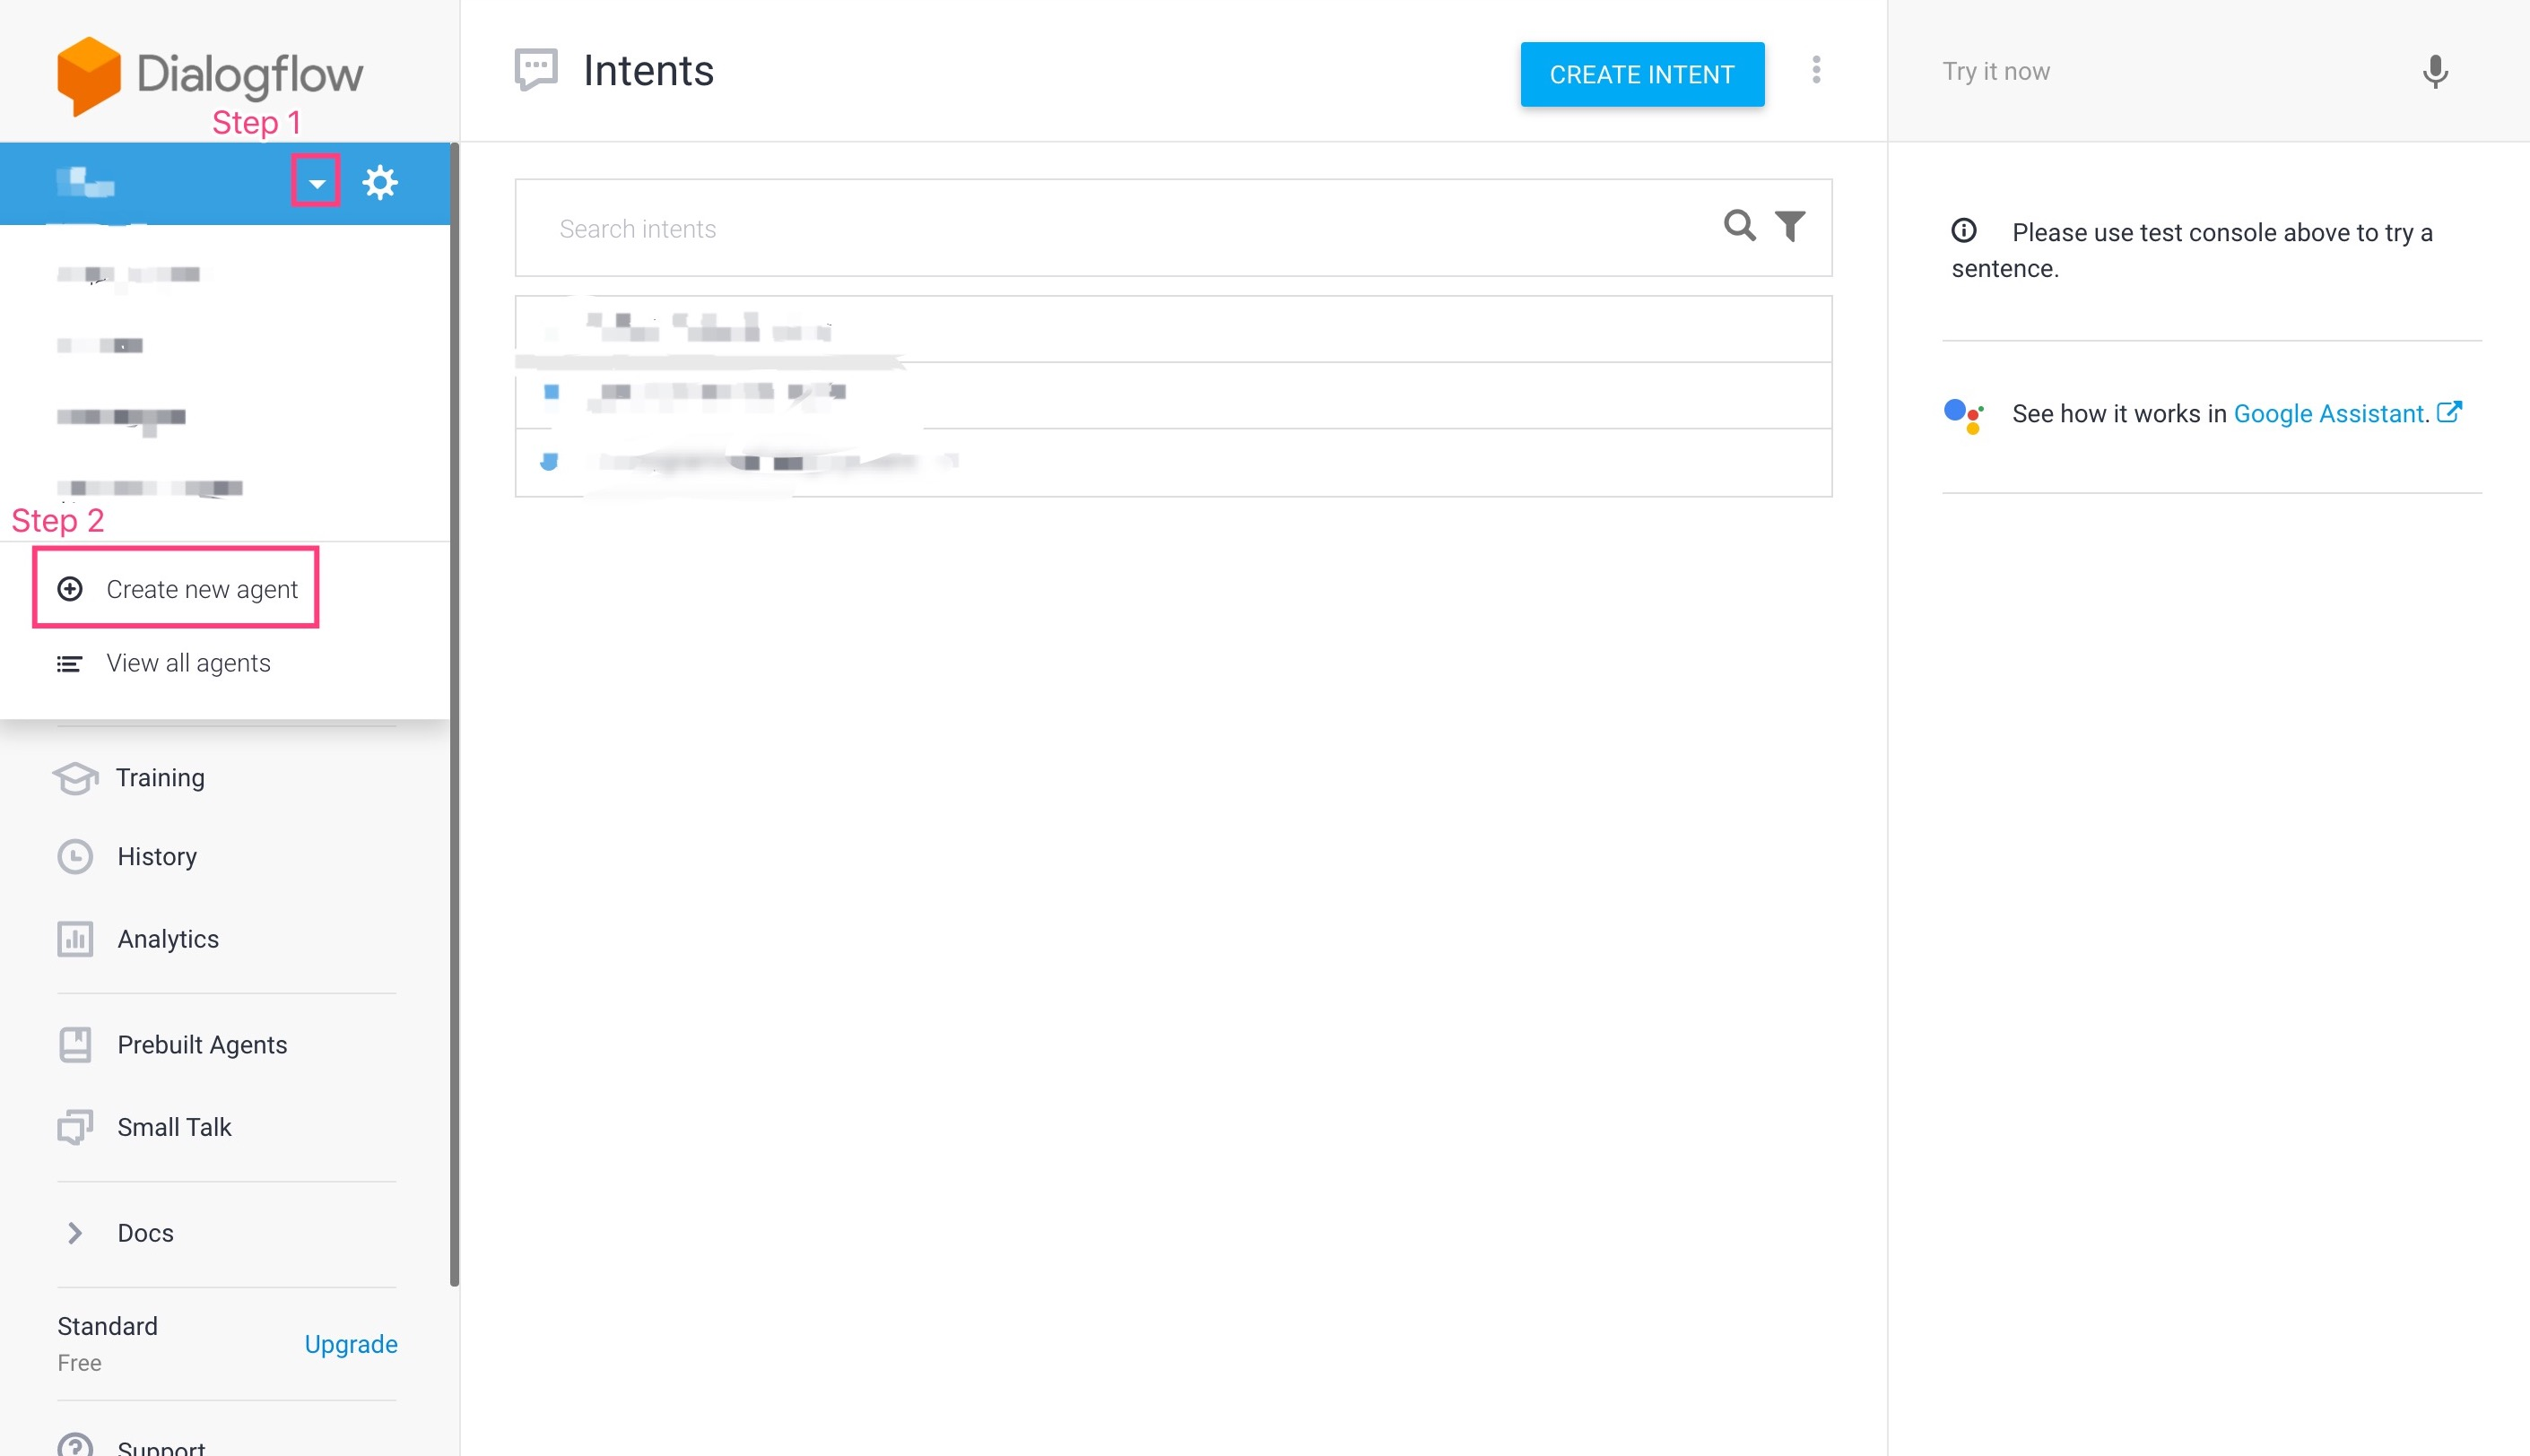
\includegraphics[width=\linewidth, frame]{img/manual_1.jpg}
	\end{figure}

	\item Put Agent name as you wish, then click “CREATE” button

	\begin{figure}[H]
		\centering
		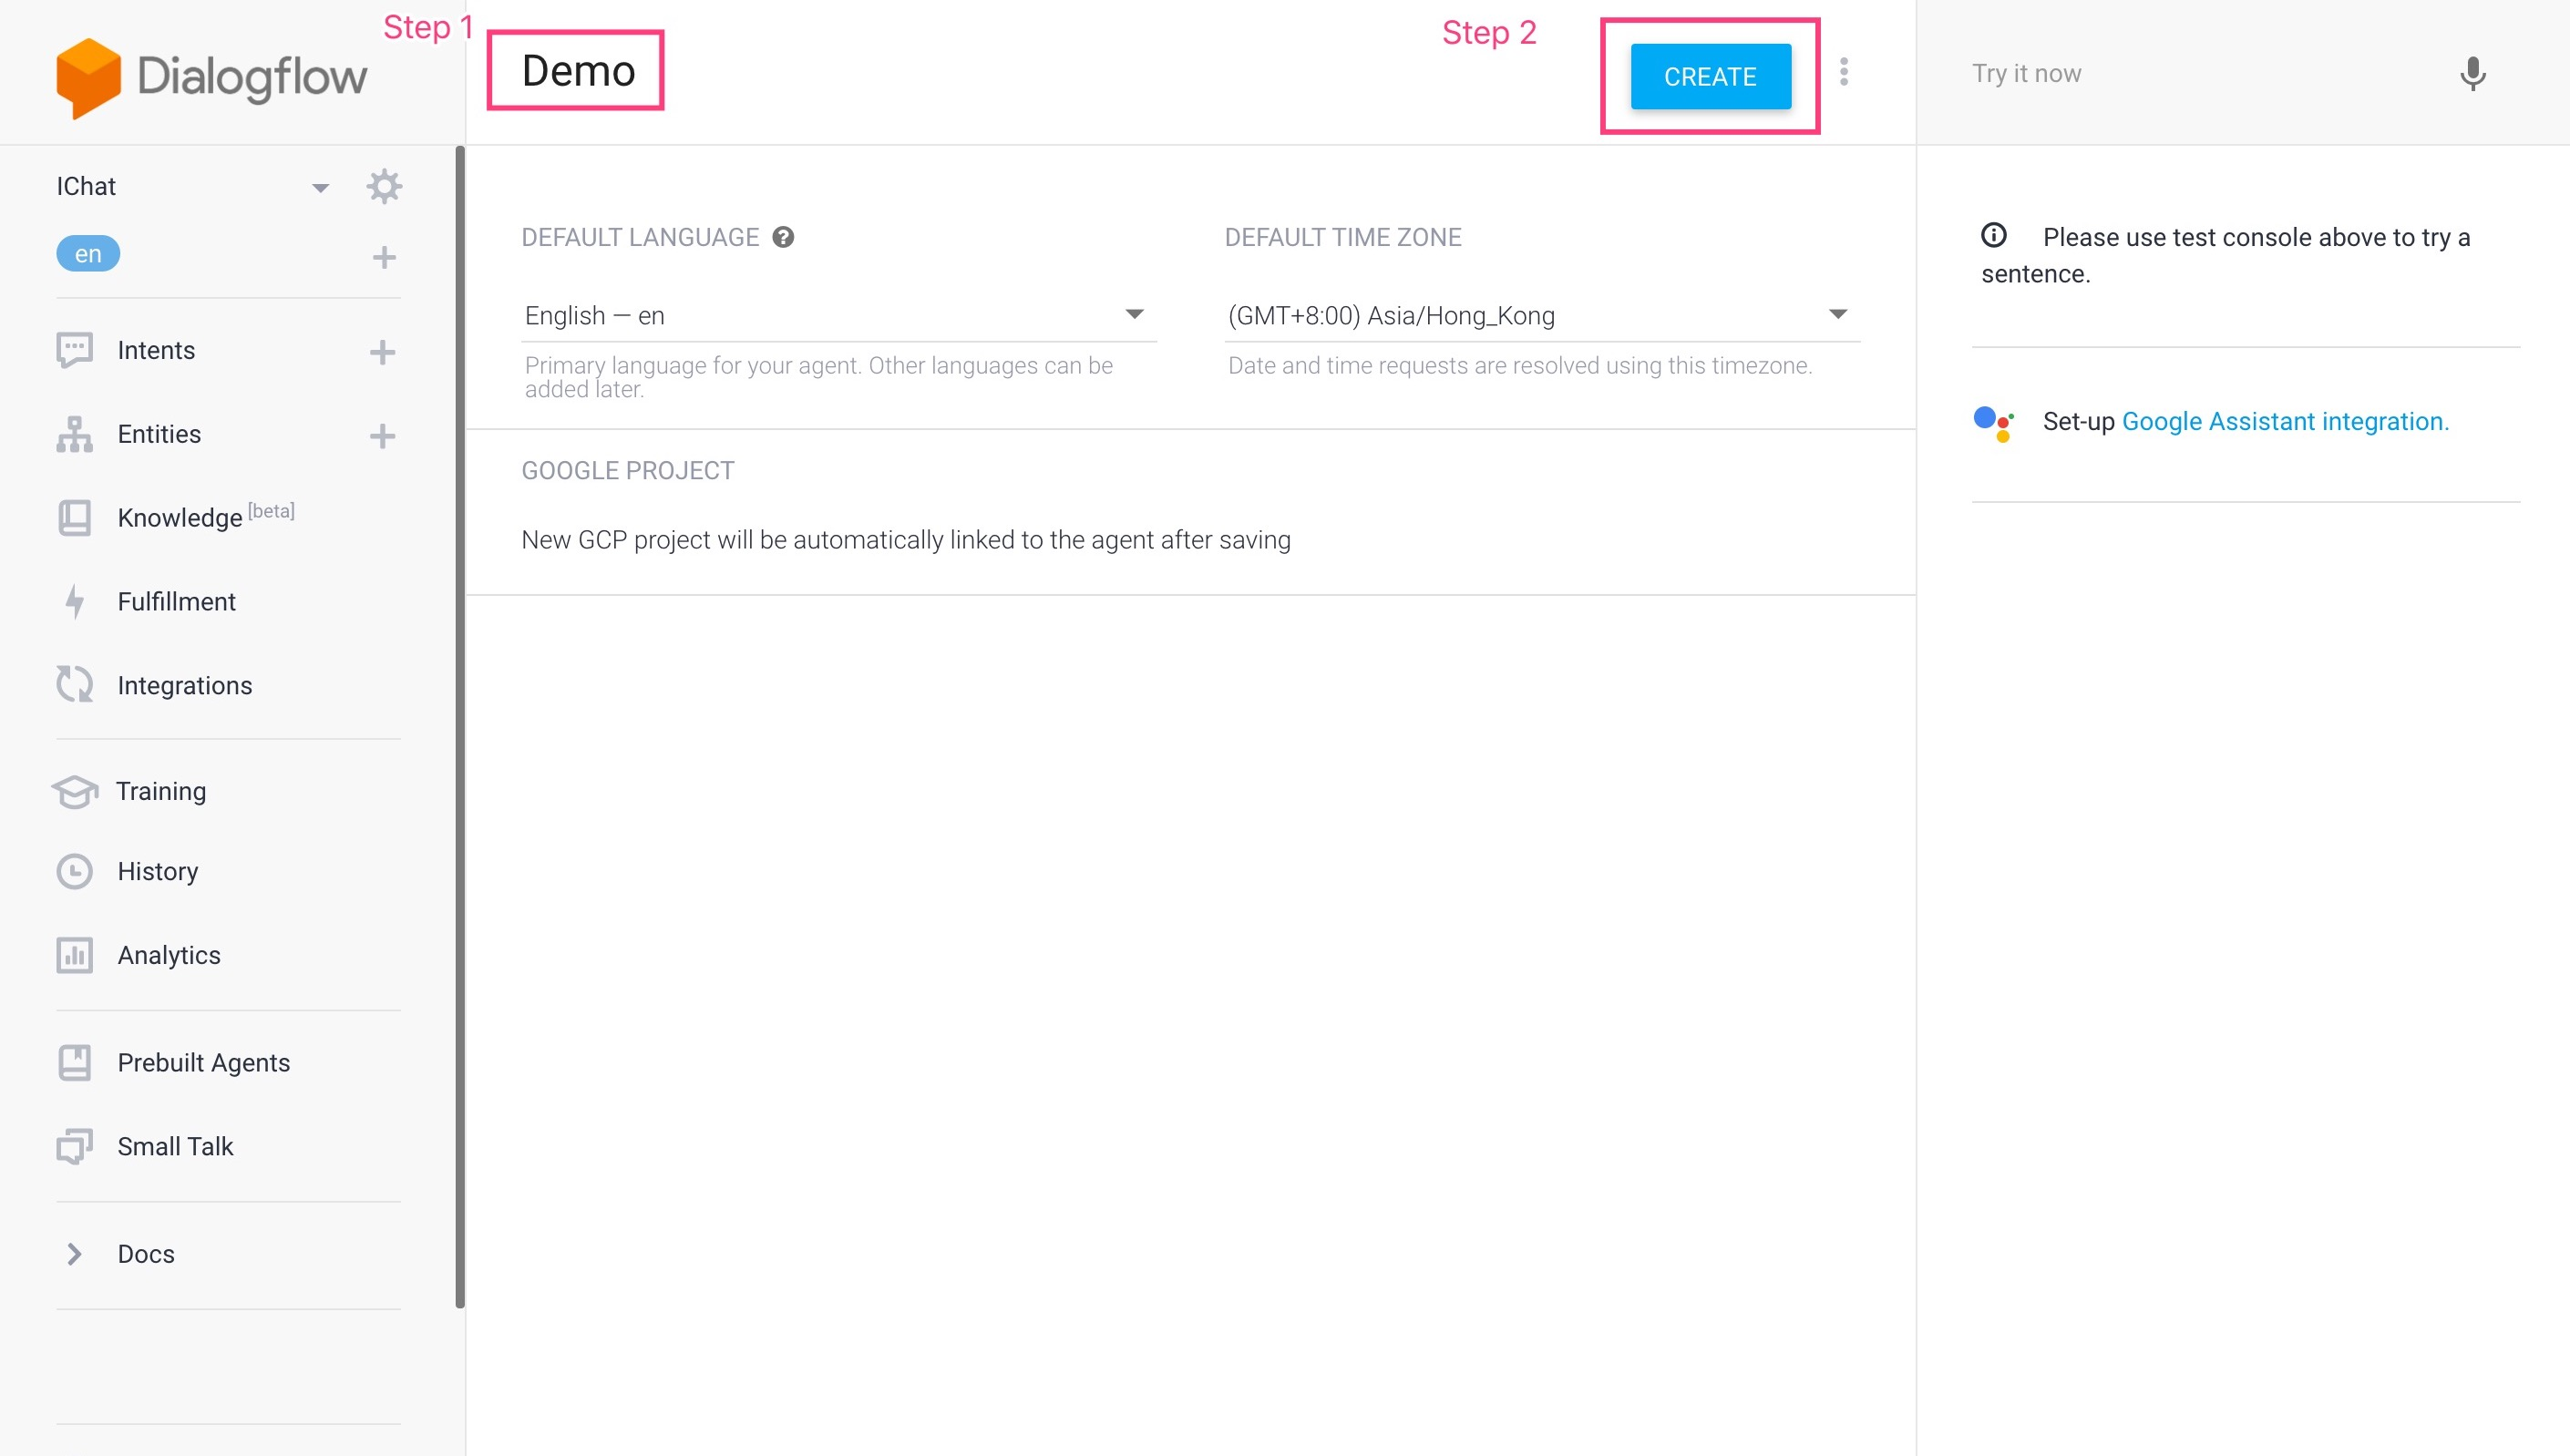
\includegraphics[width=\linewidth, frame]{img/manual_2.jpg}
	\end{figure}

	\item Go to Settings and enable beta features and APIs
	\nopagebreak
	\begin{figure}[H]
		\centering
		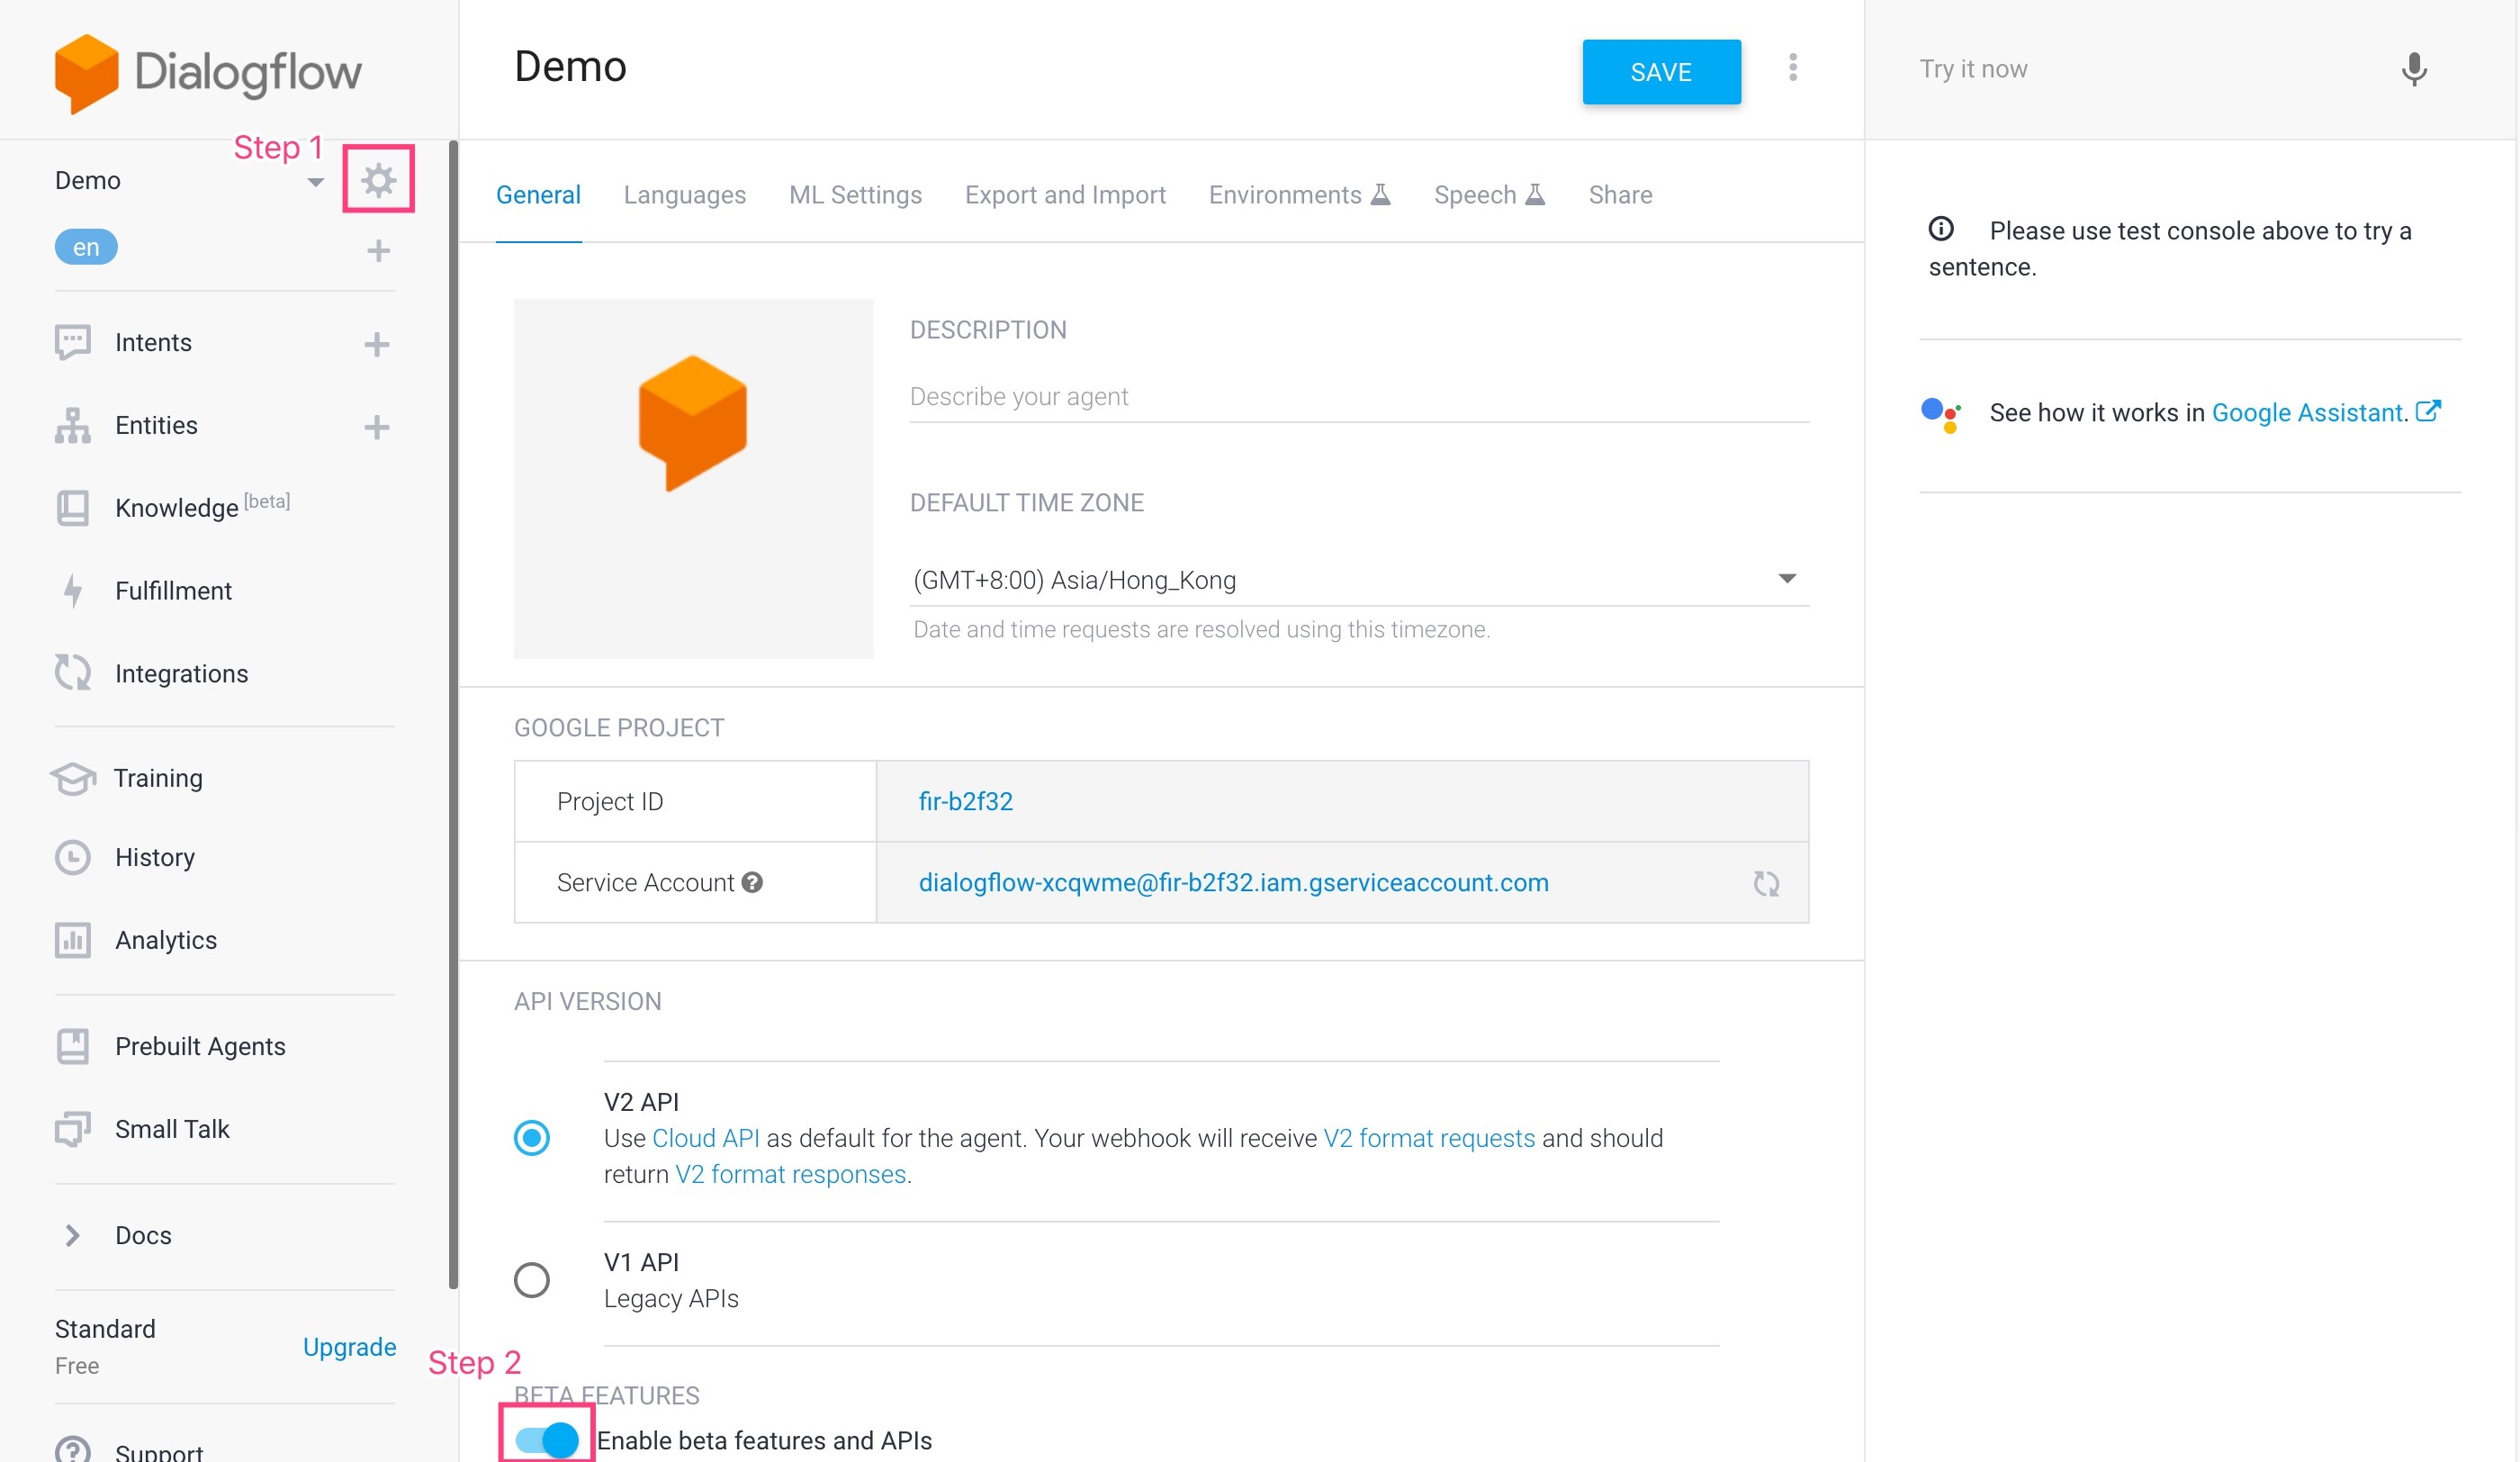
\includegraphics[width=\linewidth, frame]{img/manual_3.jpg}
	\end{figure}

	\item Go to “Export and Import” and click “IMPORT FROM ZIP”

	\begin{figure}[H]
		\centering
		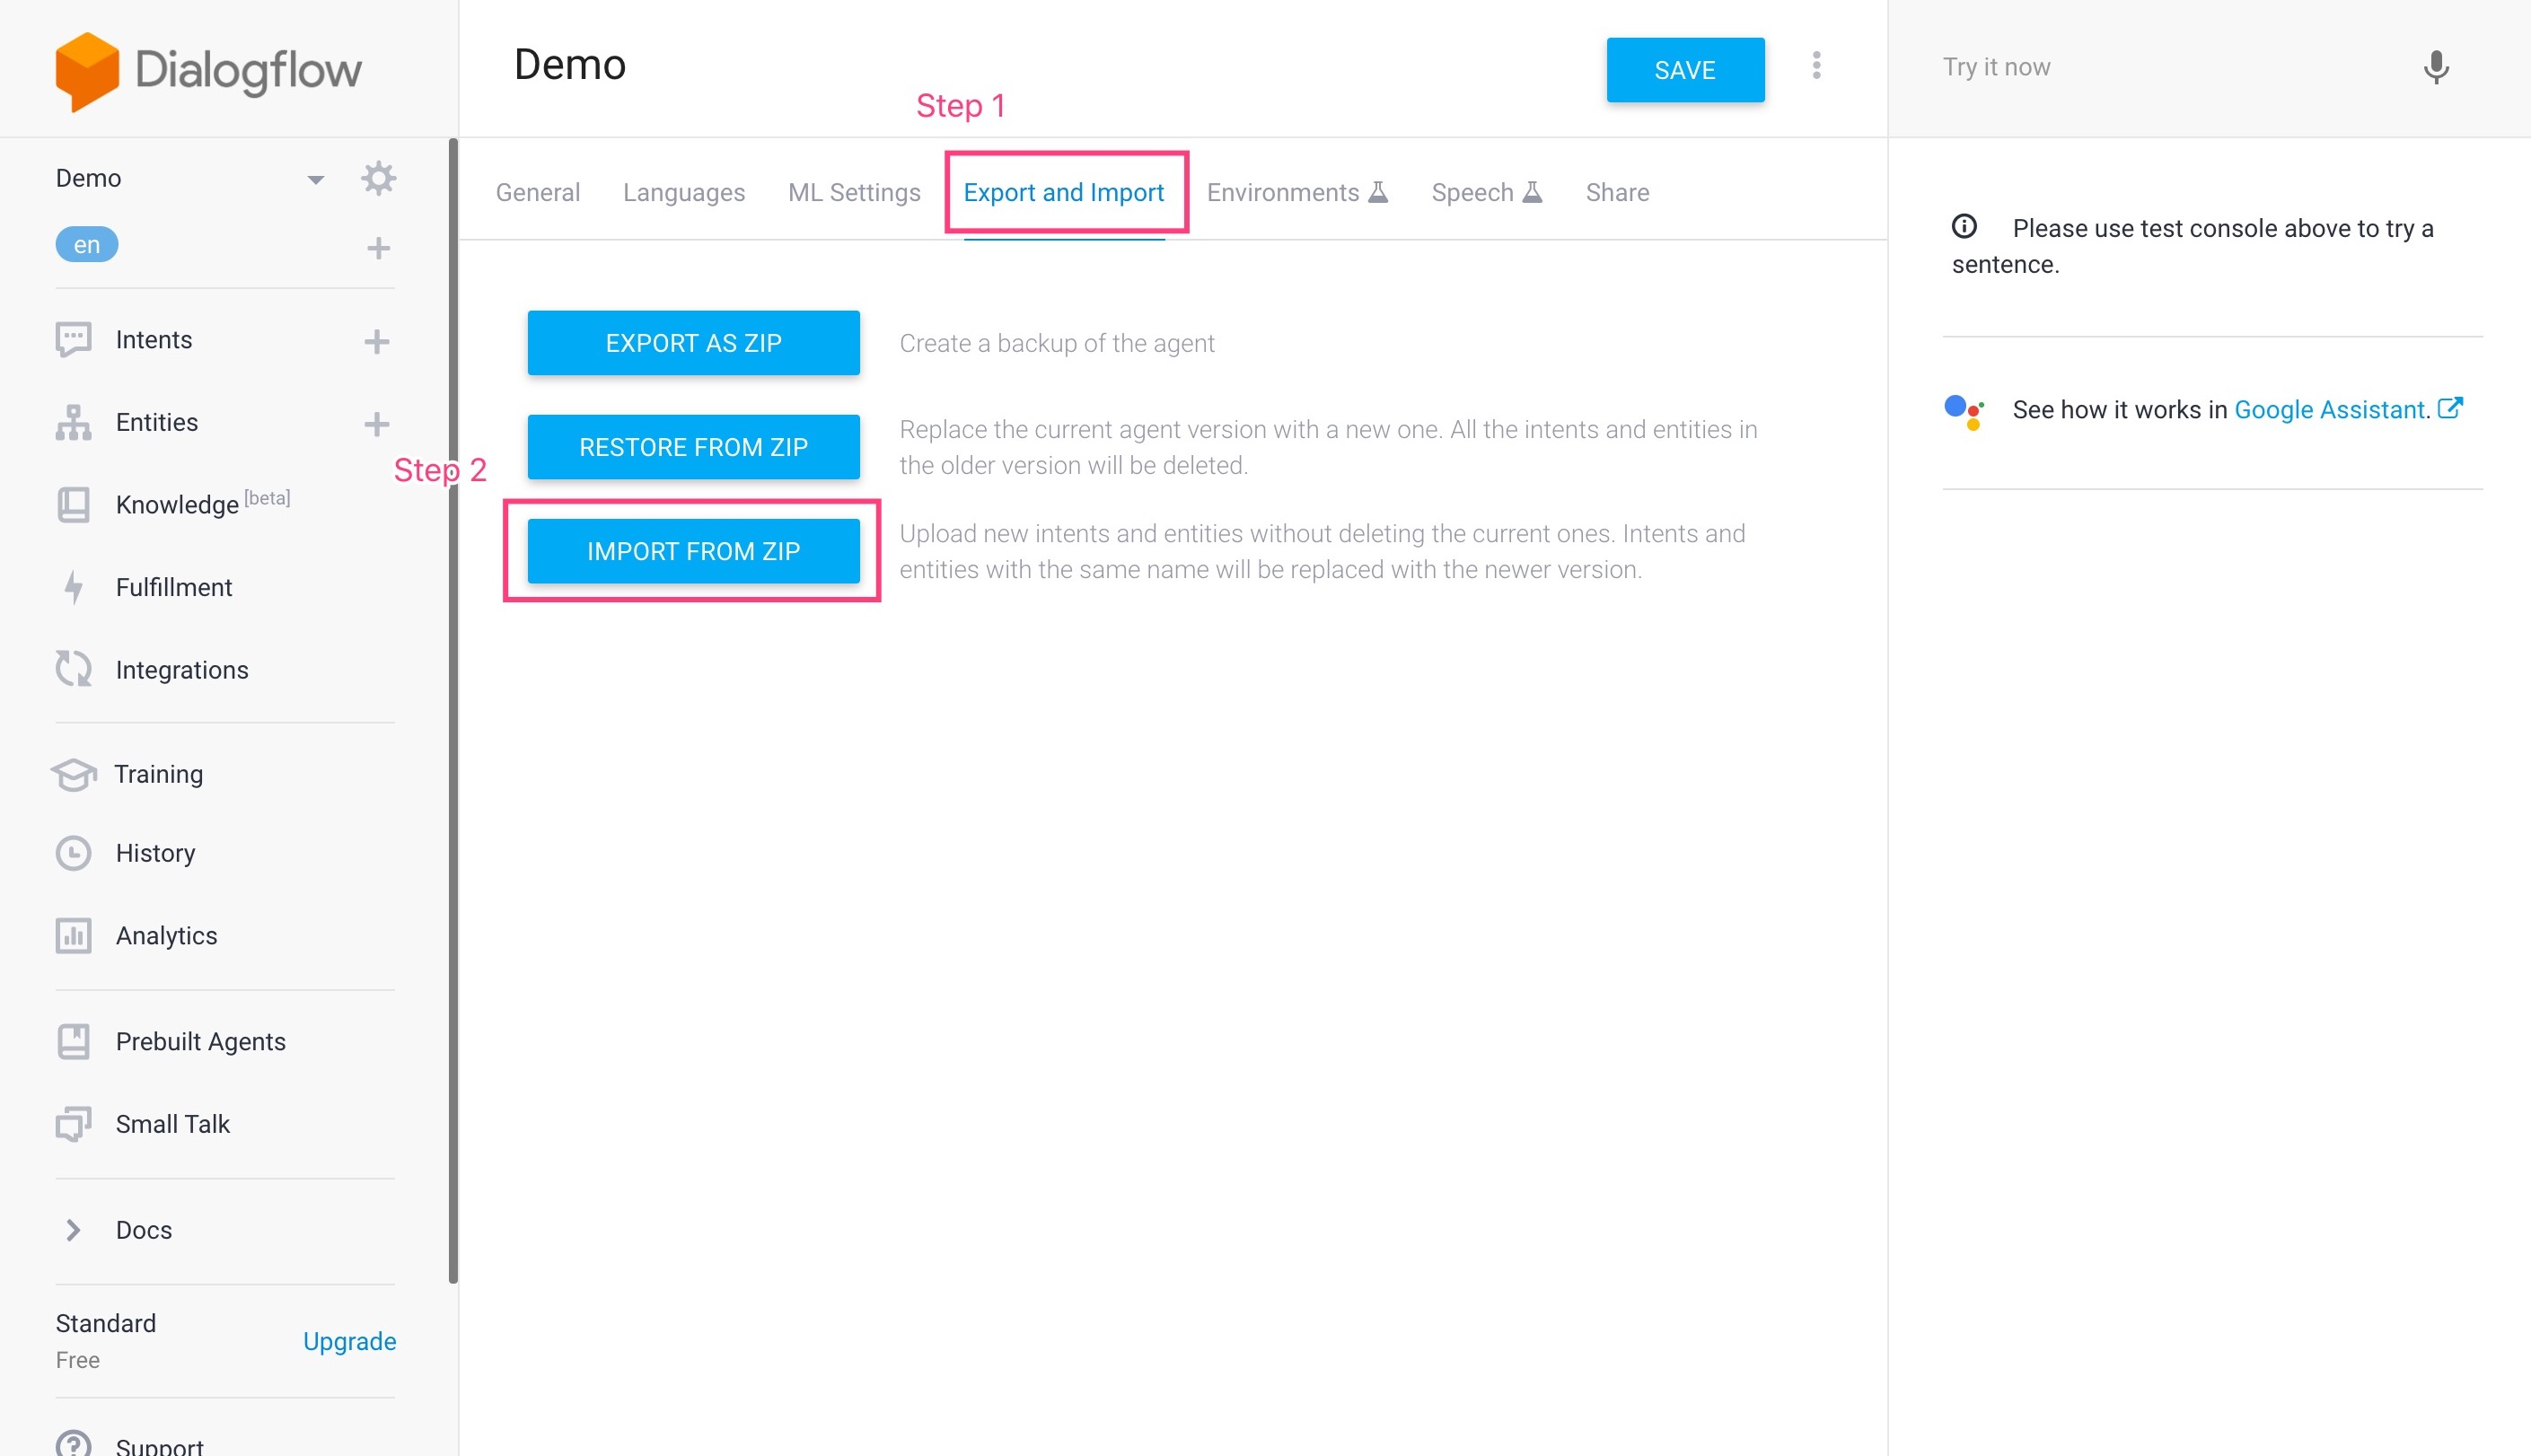
\includegraphics[width=\linewidth, frame]{img/manual_4.jpg}
	\end{figure}

	\item Click “SELECT FILE”
	\nopagebreak
	\begin{figure}[H]
		\centering
		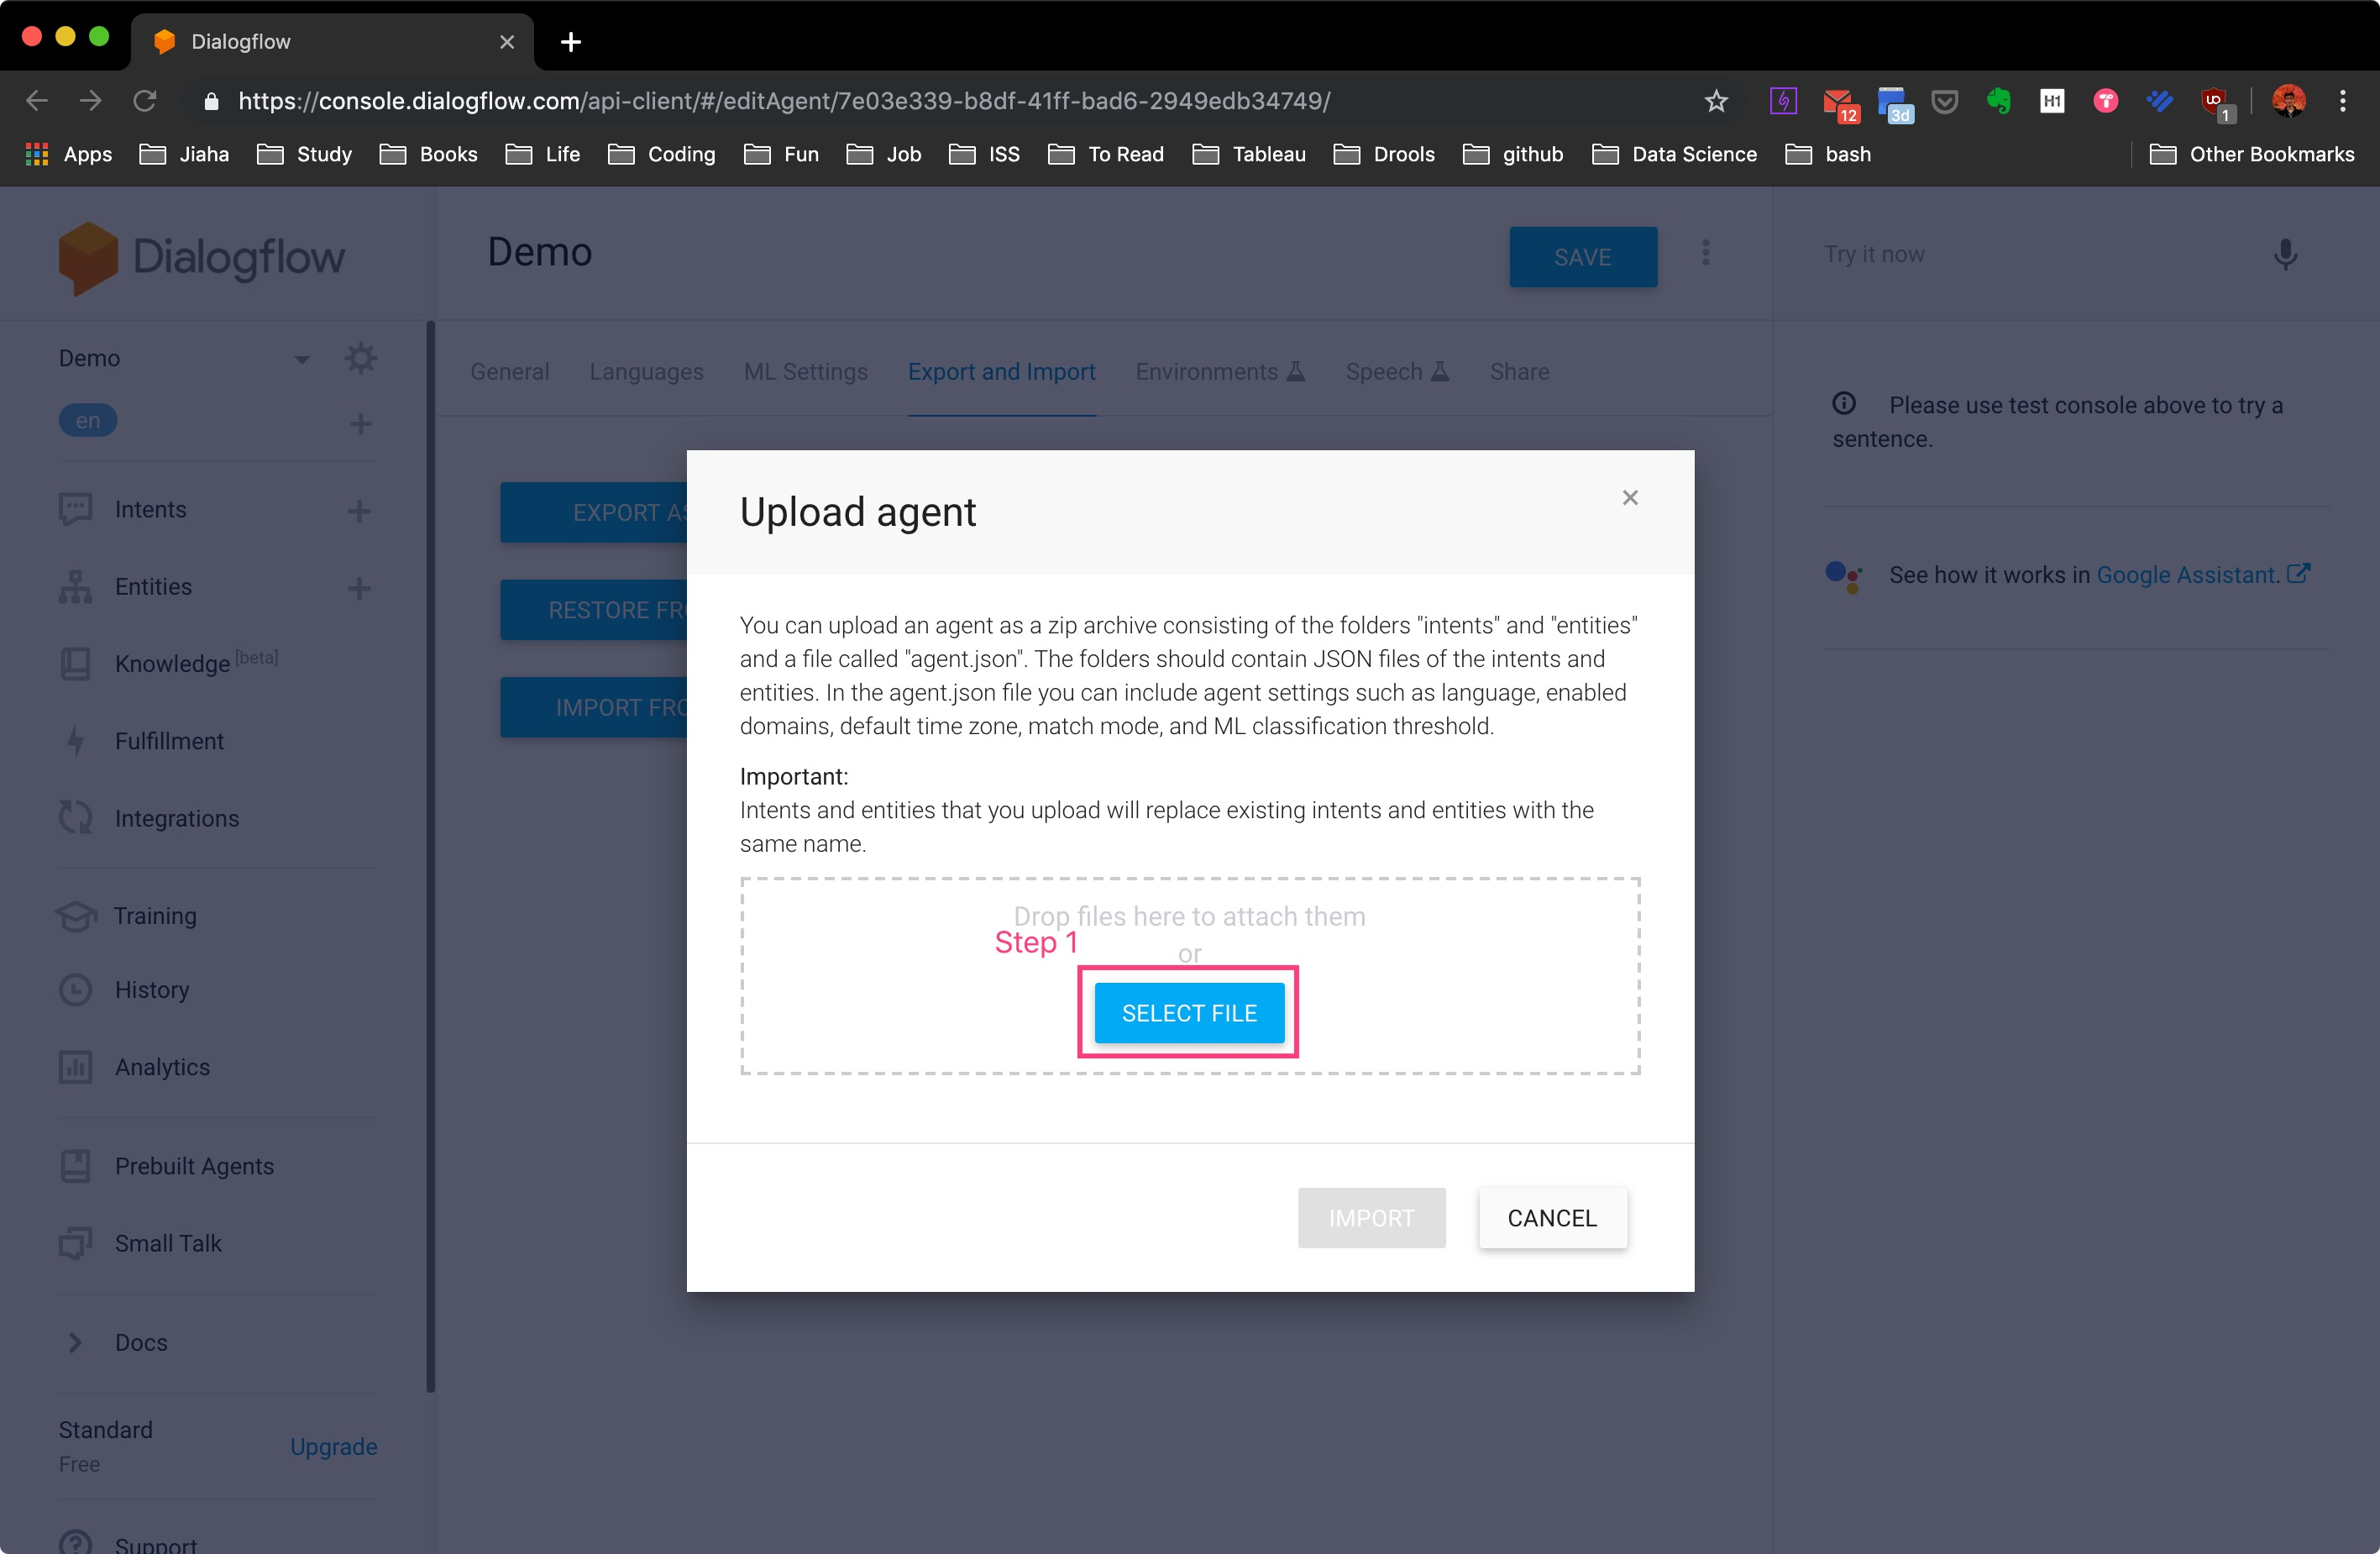
\includegraphics[width=\linewidth, frame]{img/manual_5.jpg}
	\end{figure}

	\item Choose “IChat.zip”, type IMPORT and click “IMPORT” button. Click “Done” button once imported.

	\begin{figure}[H]
		\centering
		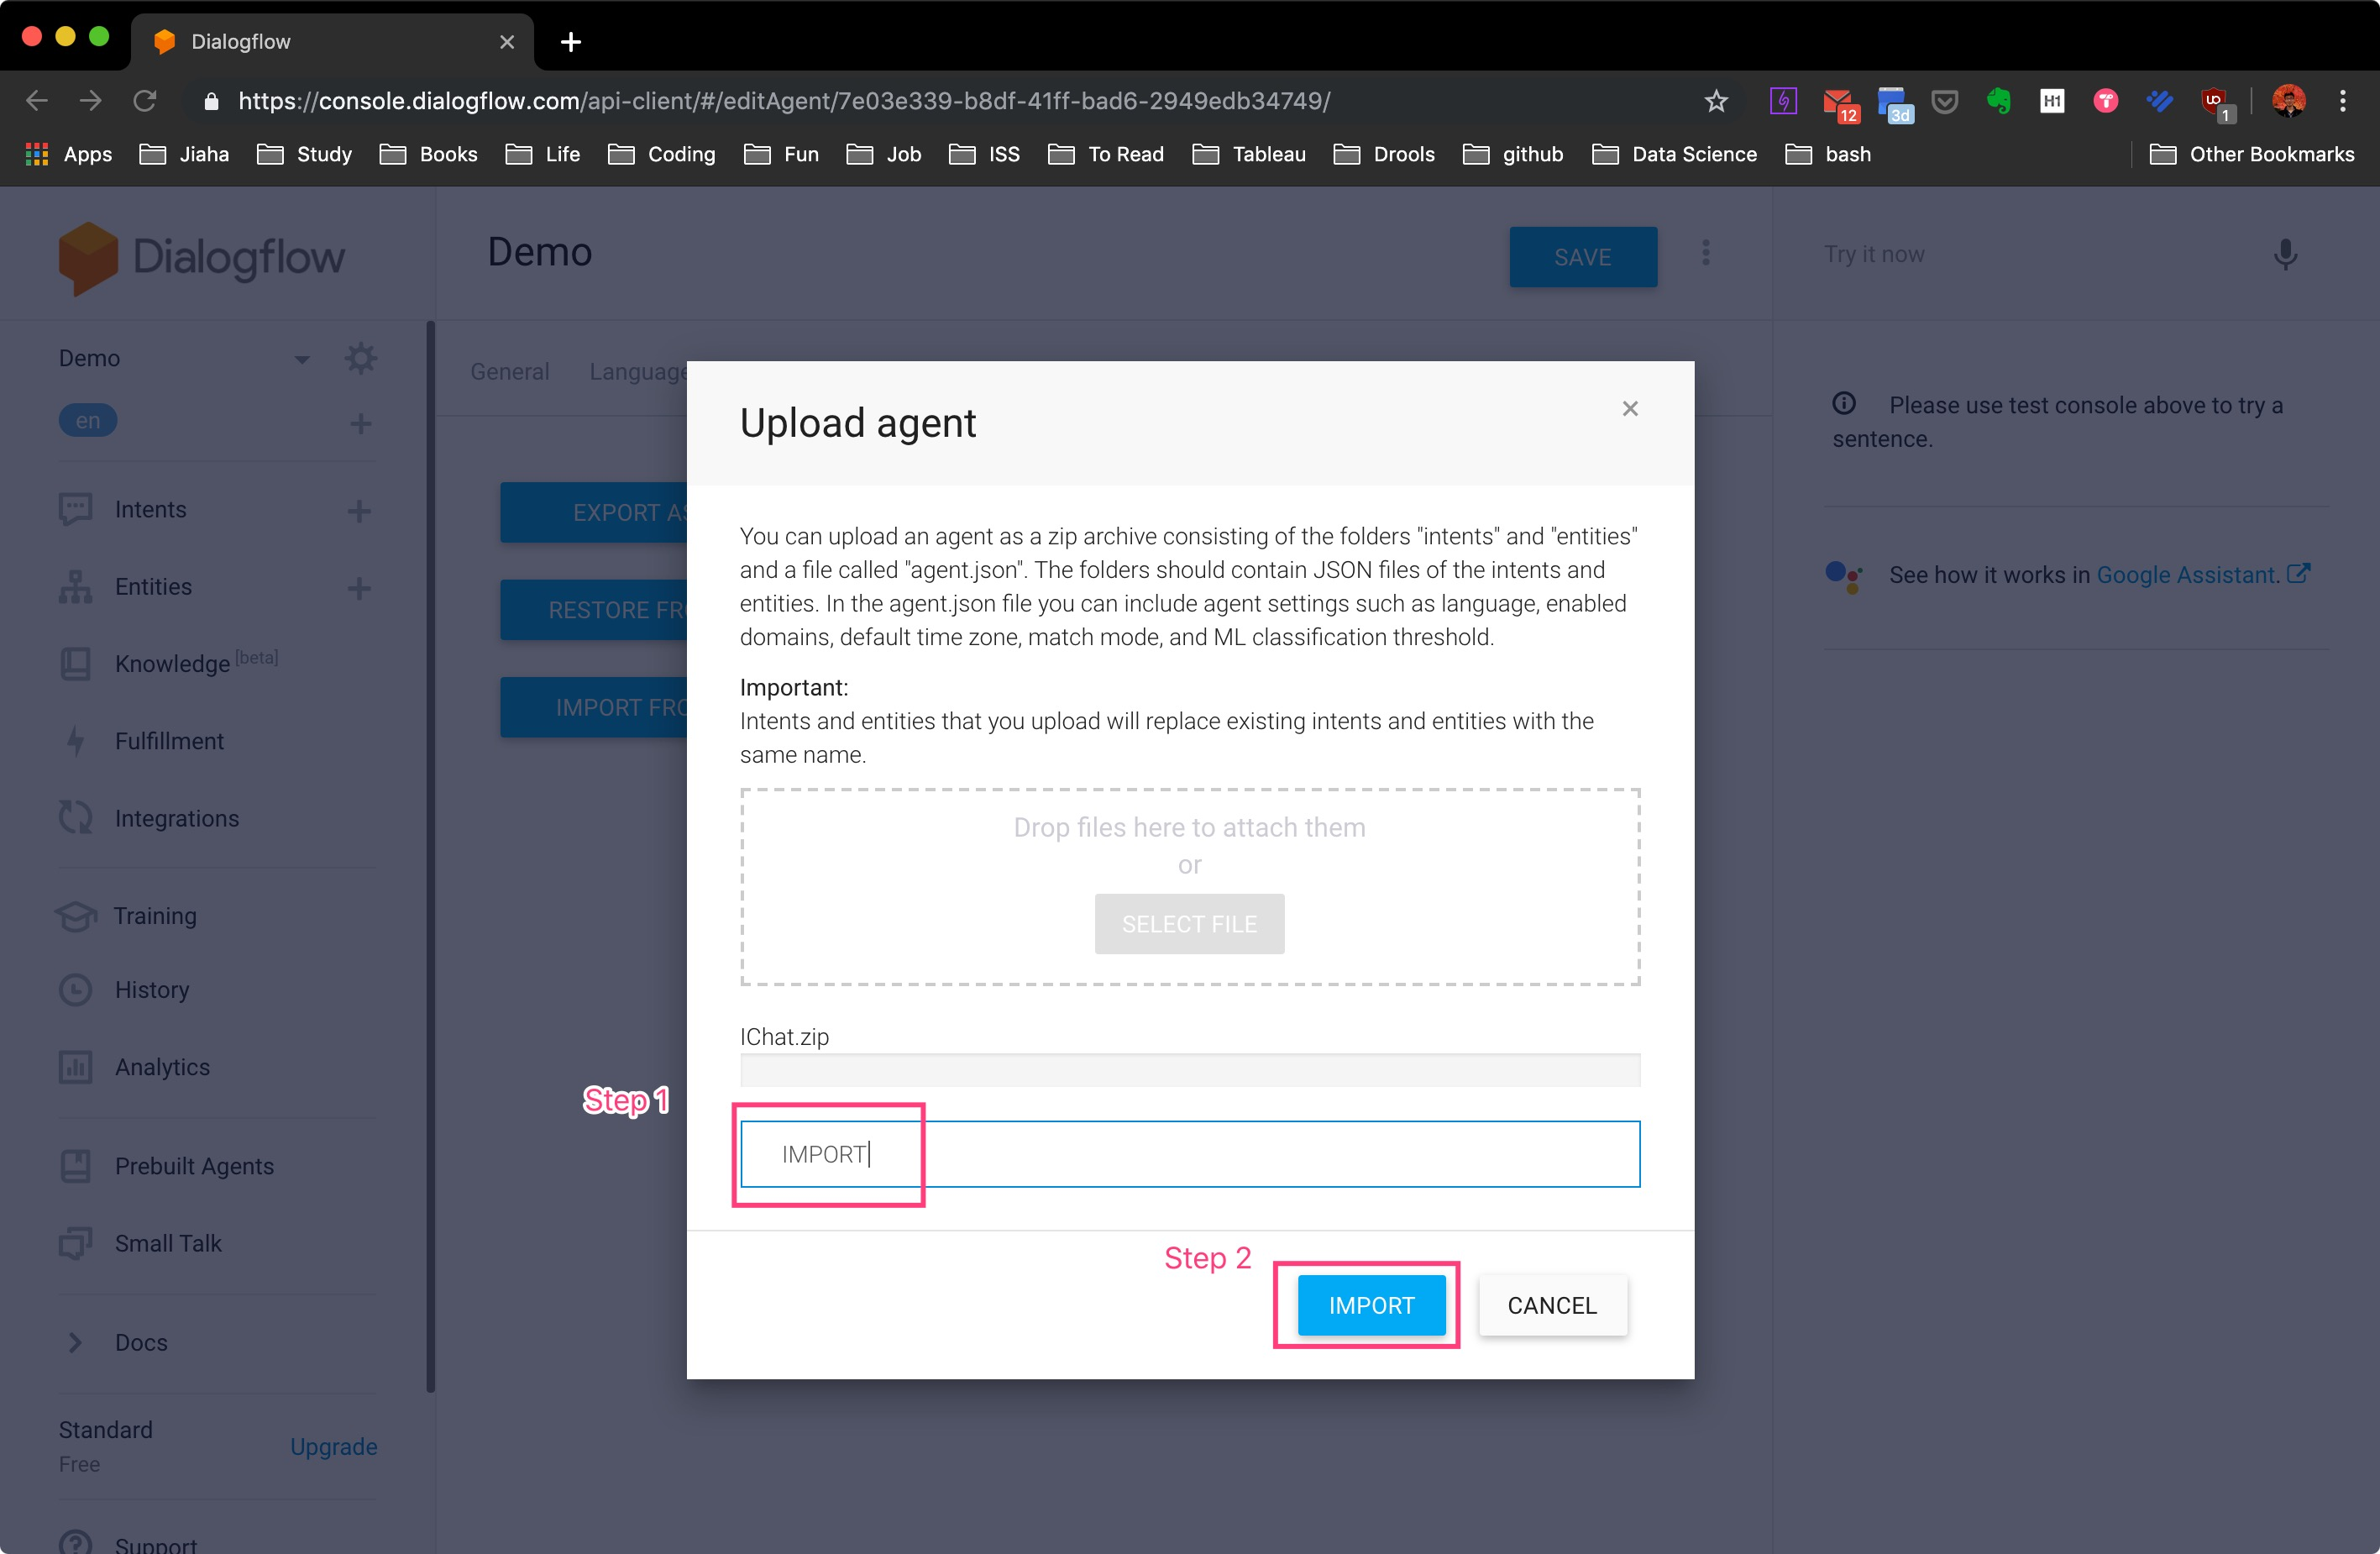
\includegraphics[width=\linewidth, frame]{img/manual_6.jpg}
	\end{figure}
\end{enumerate}
% section import_agent (end)

So far the “Intent” and “Entities” should be all imported into this agent.
Let’s continue to import “knowledge”.

\section{Create Knowledge} % (fold)
\label{sec:create_knowledge}
\begin{enumerate}

	\item Click “Knowledge” and then “Create the first one”

	\begin{figure}[H]
		\centering
		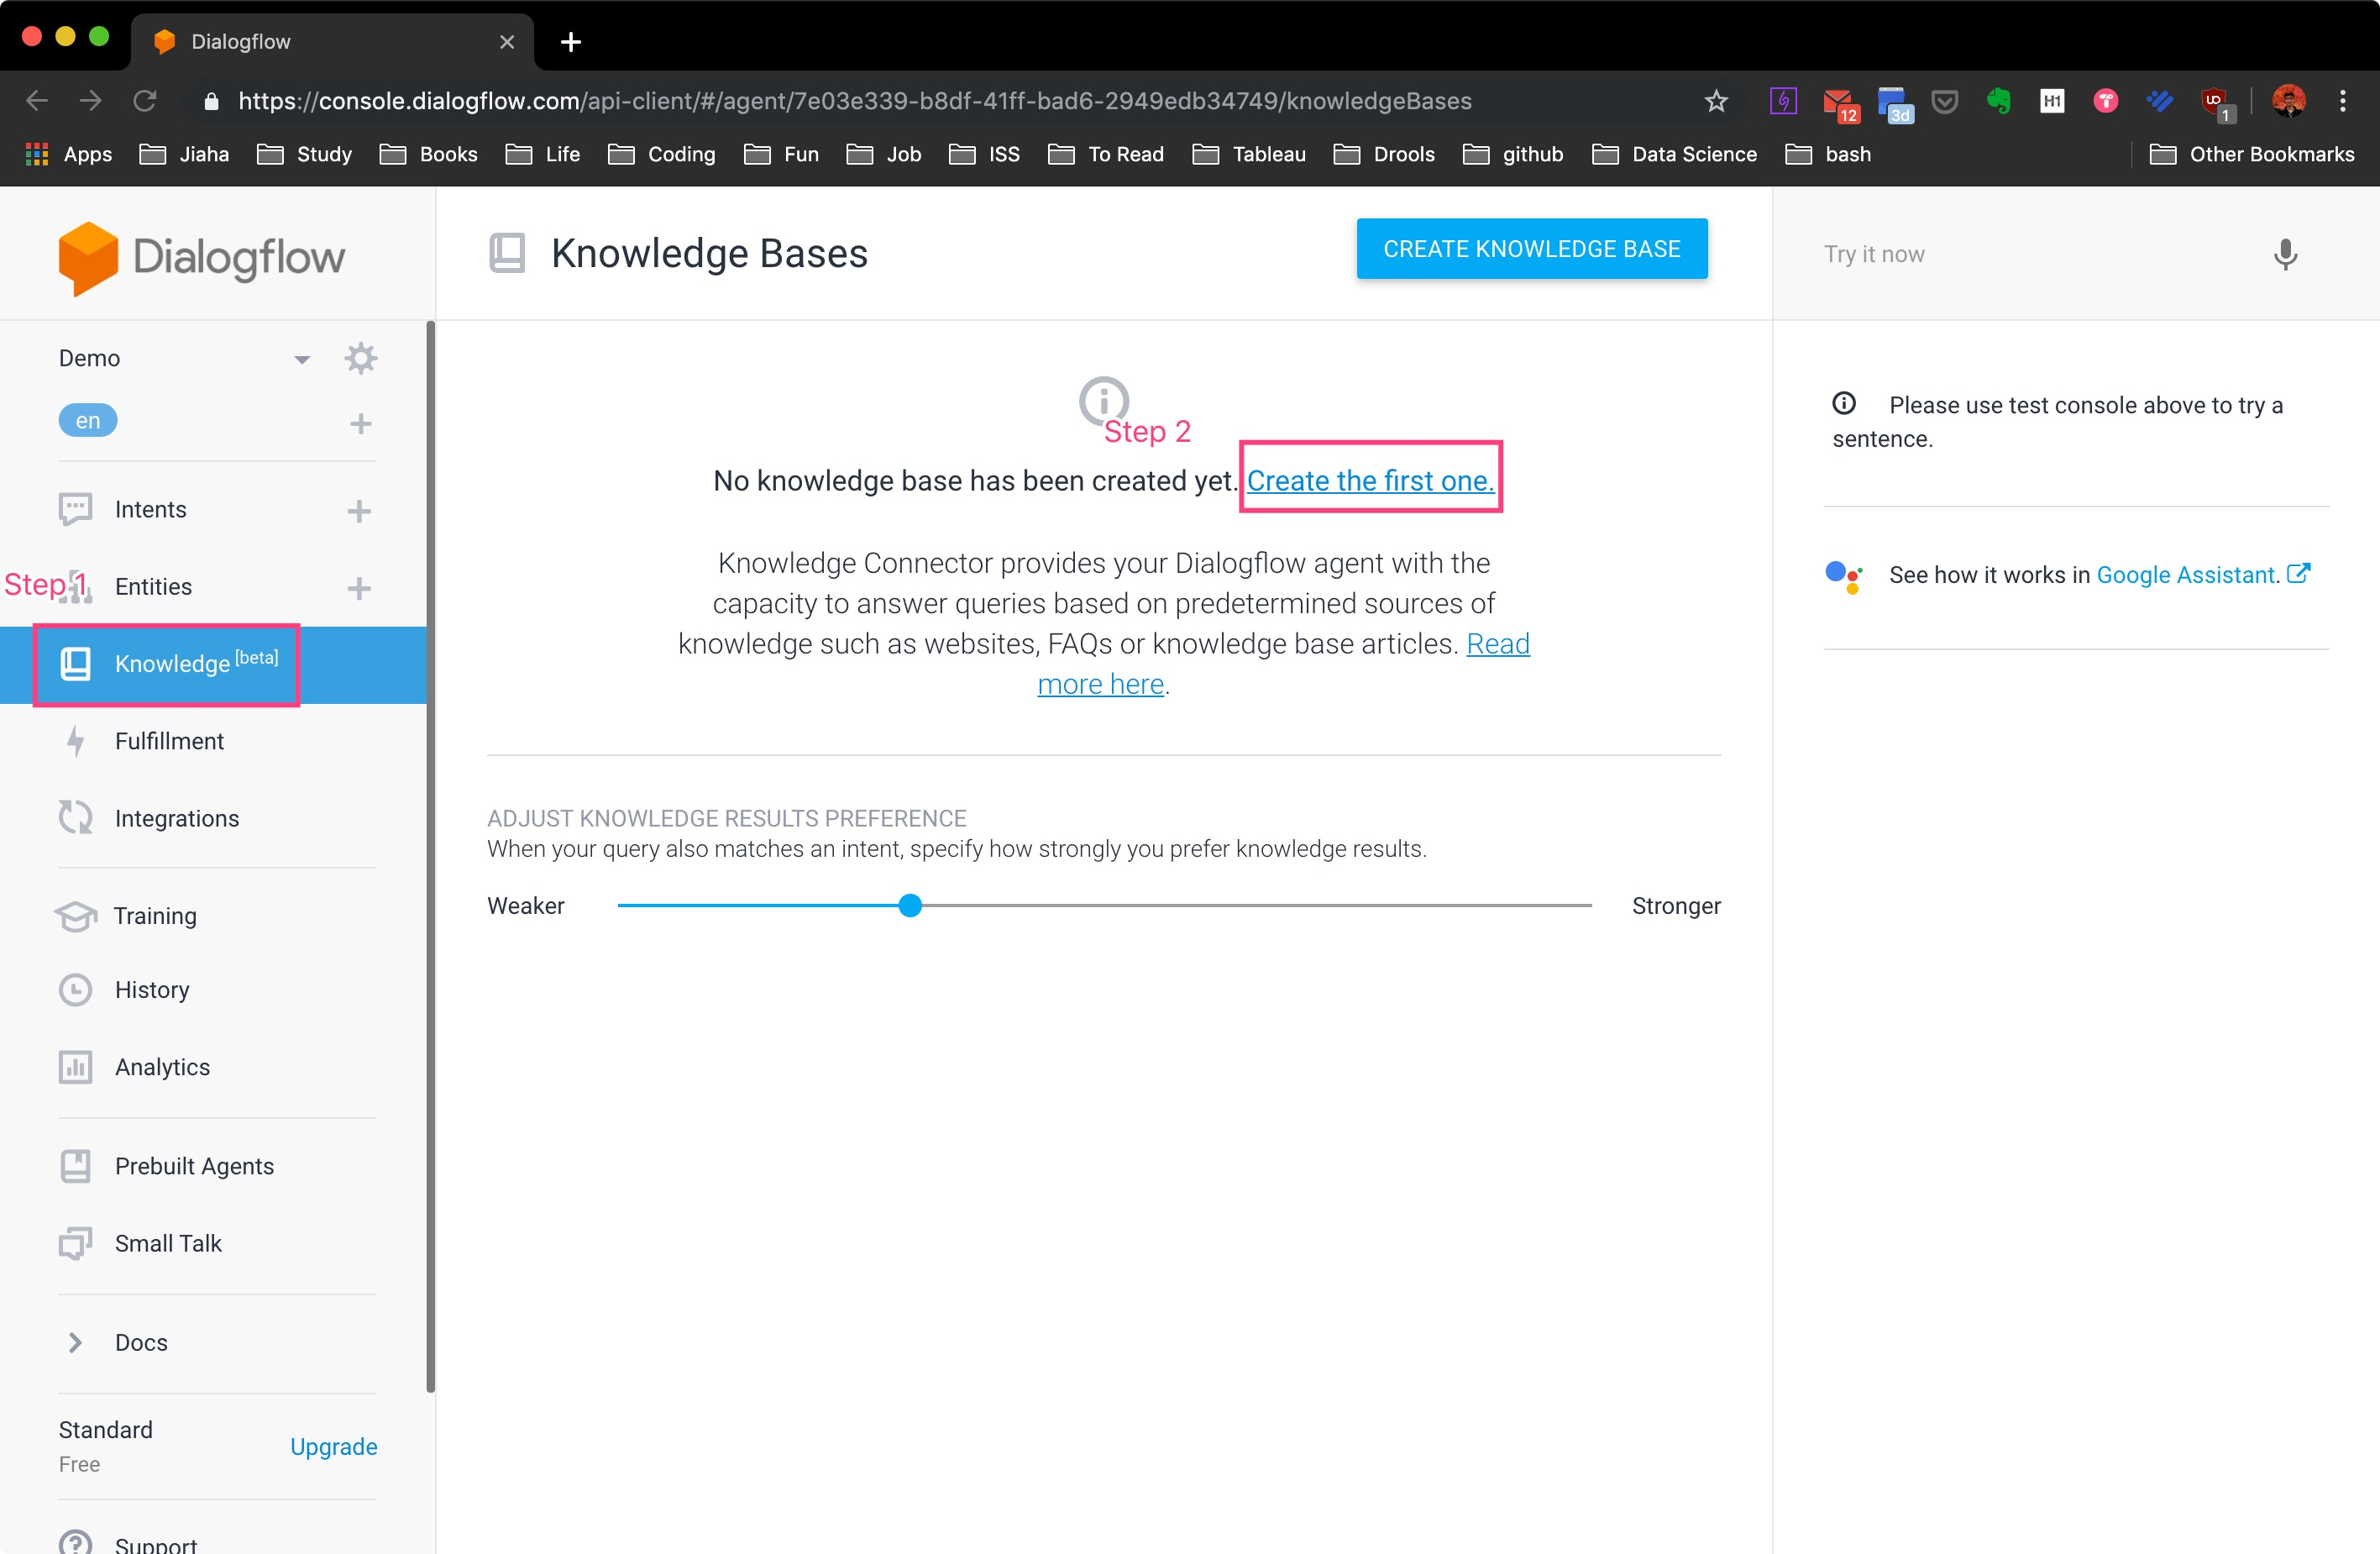
\includegraphics[width=\linewidth, frame]{img/manual_7.jpg}
	\end{figure}

	\item Put Agent name as you wish, then click “SAVE” button

	\begin{figure}[H]
		\centering
		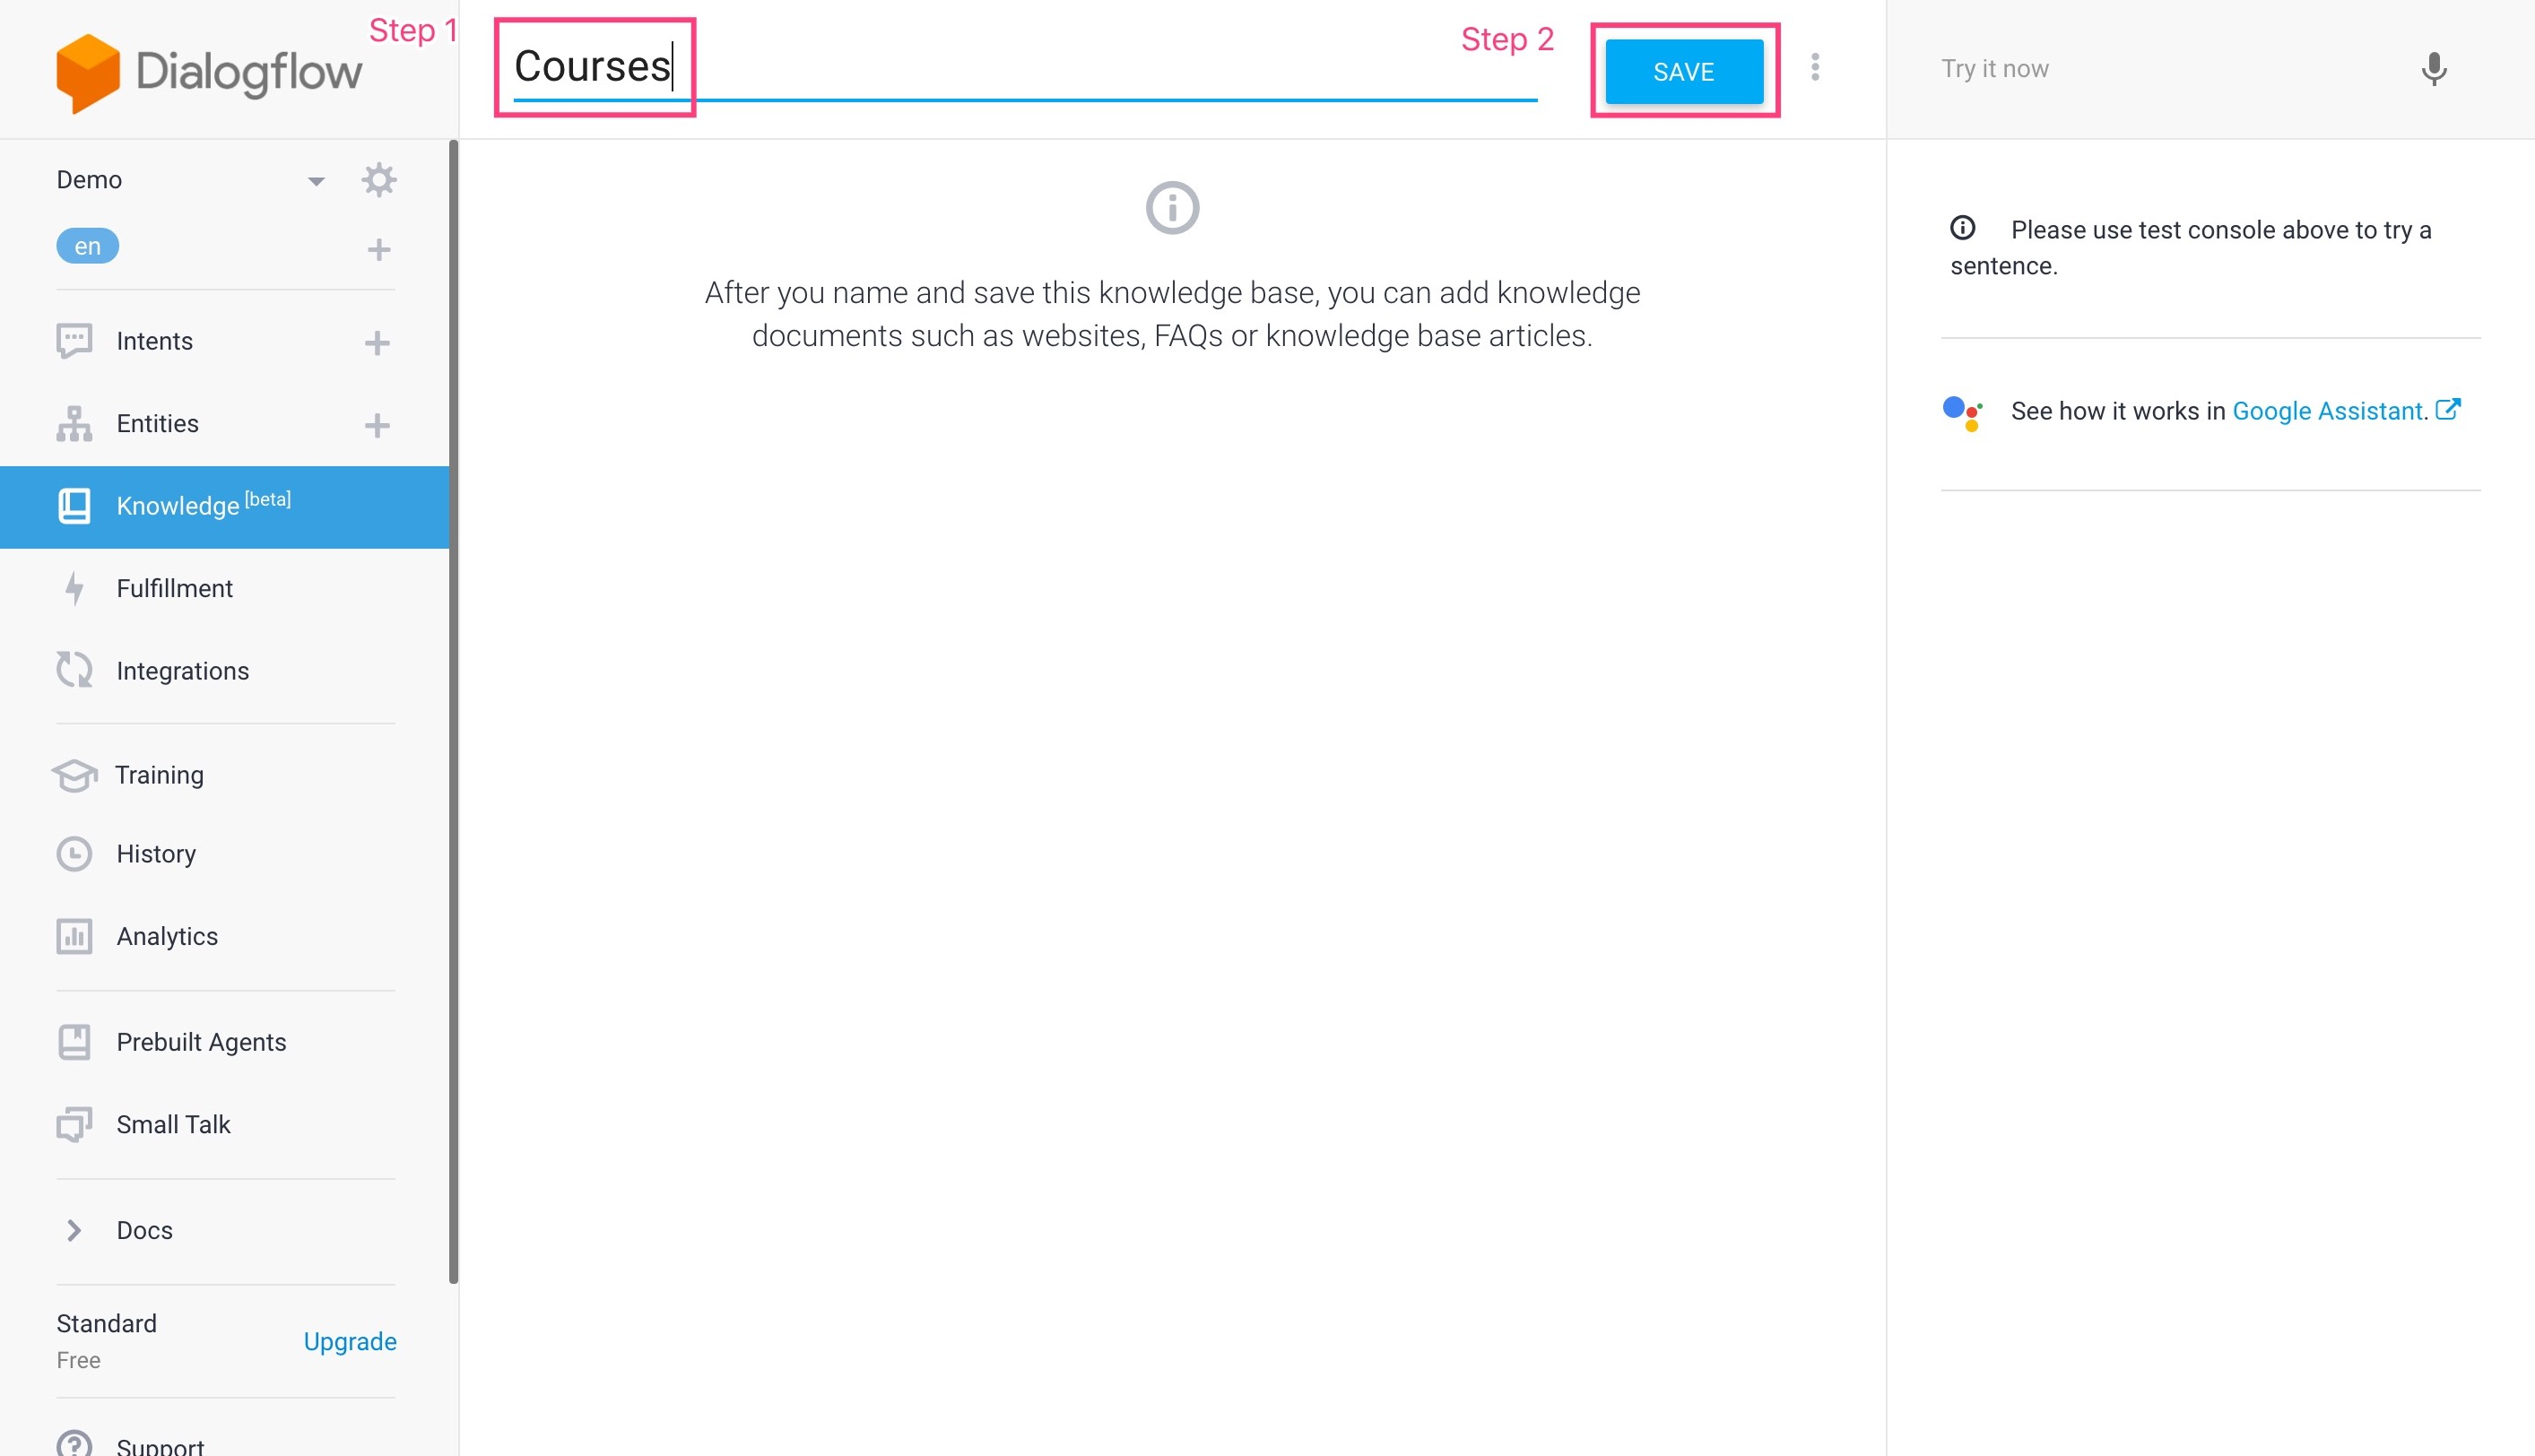
\includegraphics[width=\linewidth, frame]{img/manual_8.jpg}
	\end{figure}

	\item Click “Create the first one”
	\nopagebreak
	\begin{figure}[H]
		\centering
		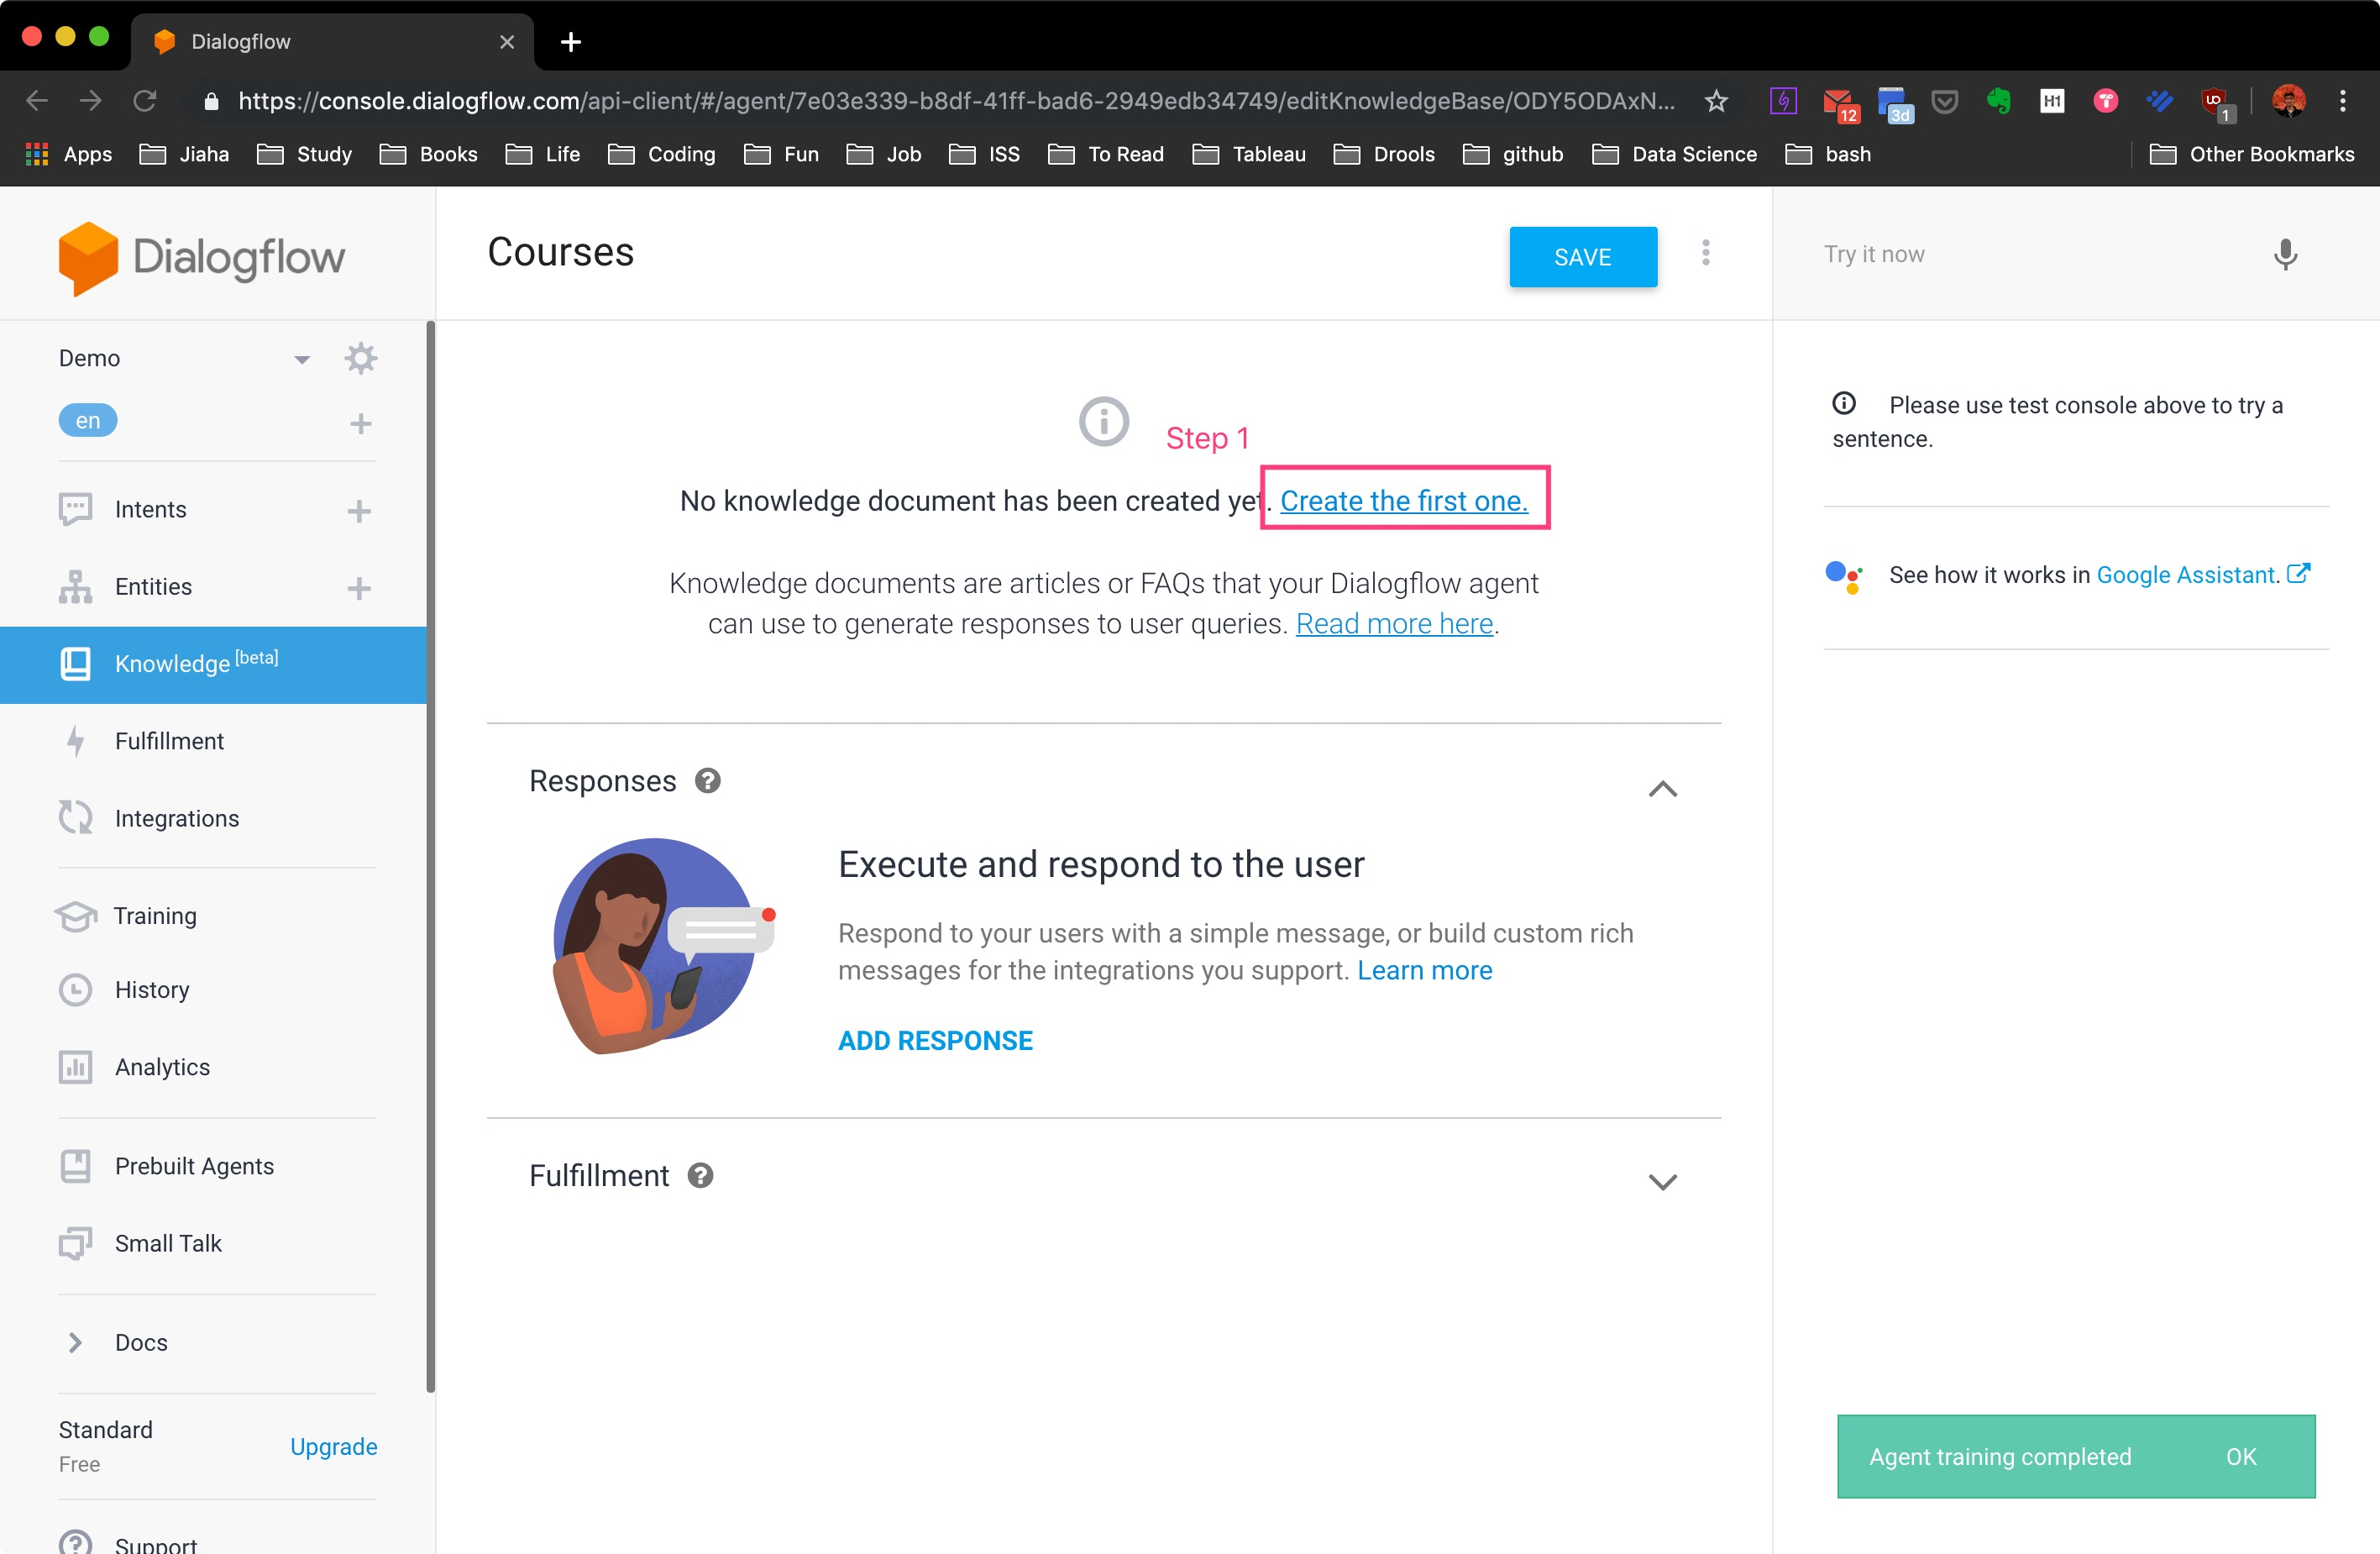
\includegraphics[width=\linewidth, frame]{img/manual_9.jpg}
	\end{figure}

	\item Input the fields as follows and upload “part1.csv”, then click “CREATE” button
	\nopagebreak
	\begin{figure}[H]
		\centering
		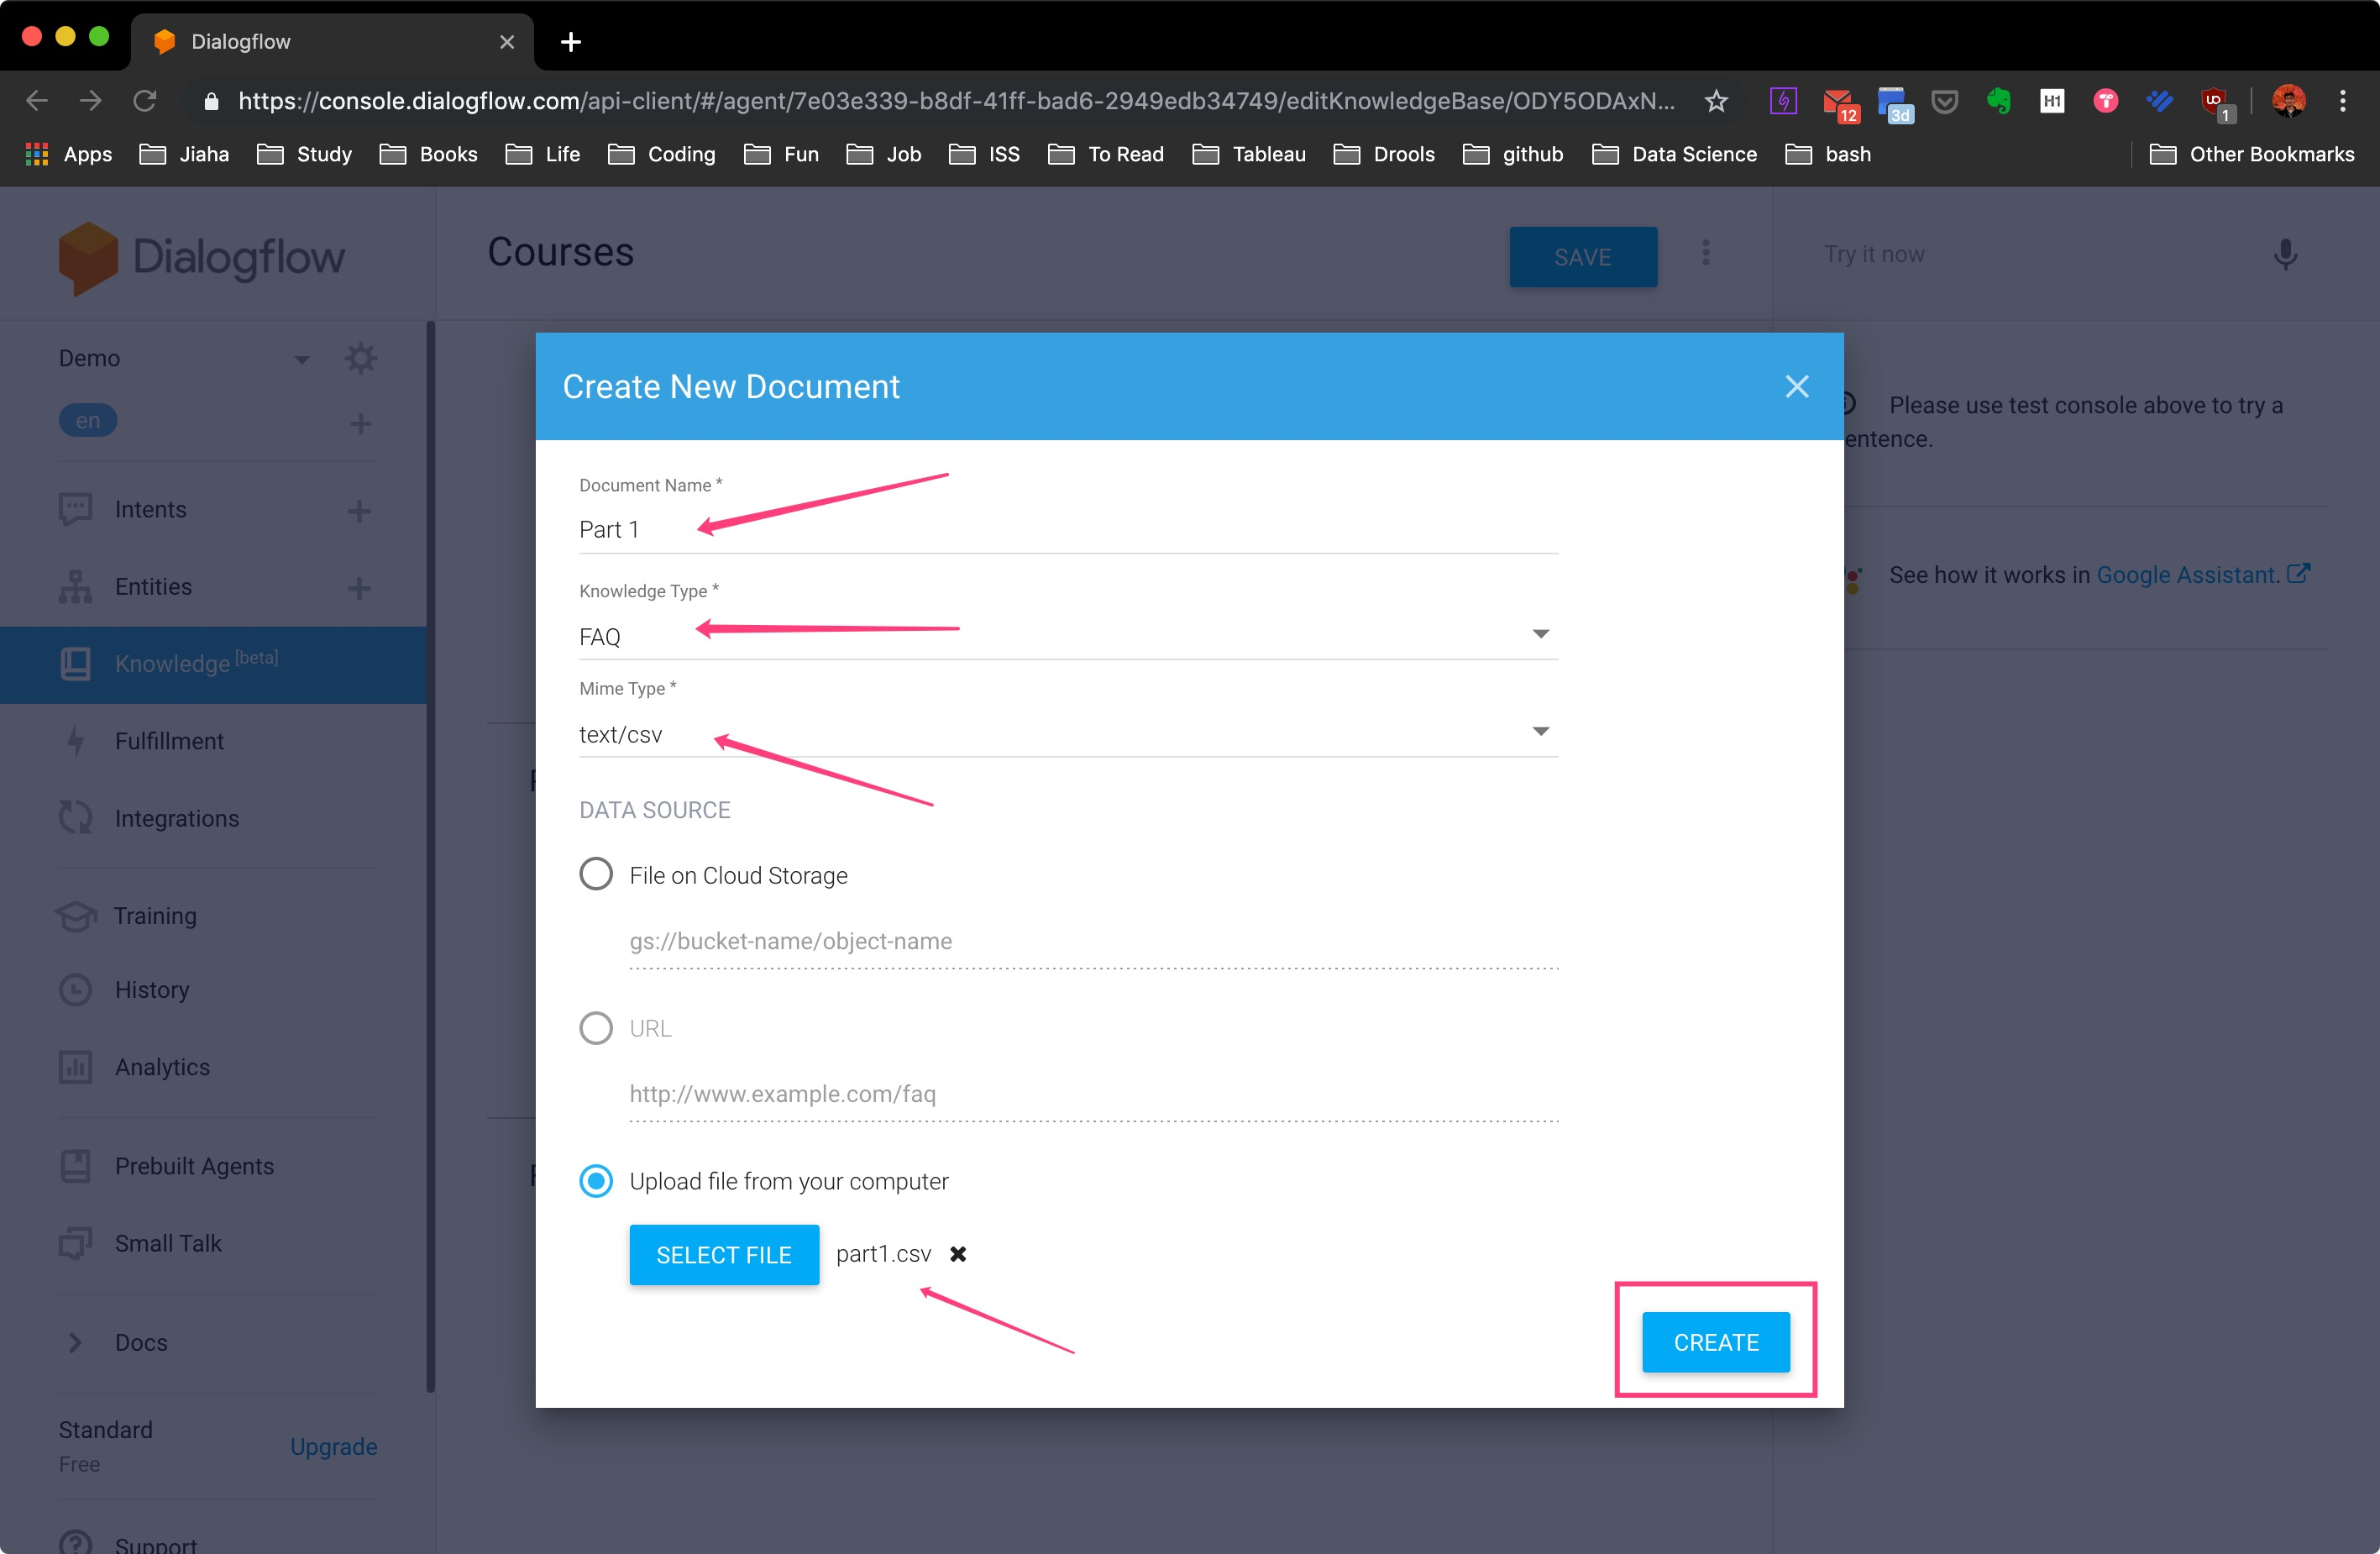
\includegraphics[width=\linewidth, frame]{img/manual_10.jpg}
	\end{figure}

	\item Click “+ New Document”
	\nopagebreak
	\begin{figure}[H]
		\centering
		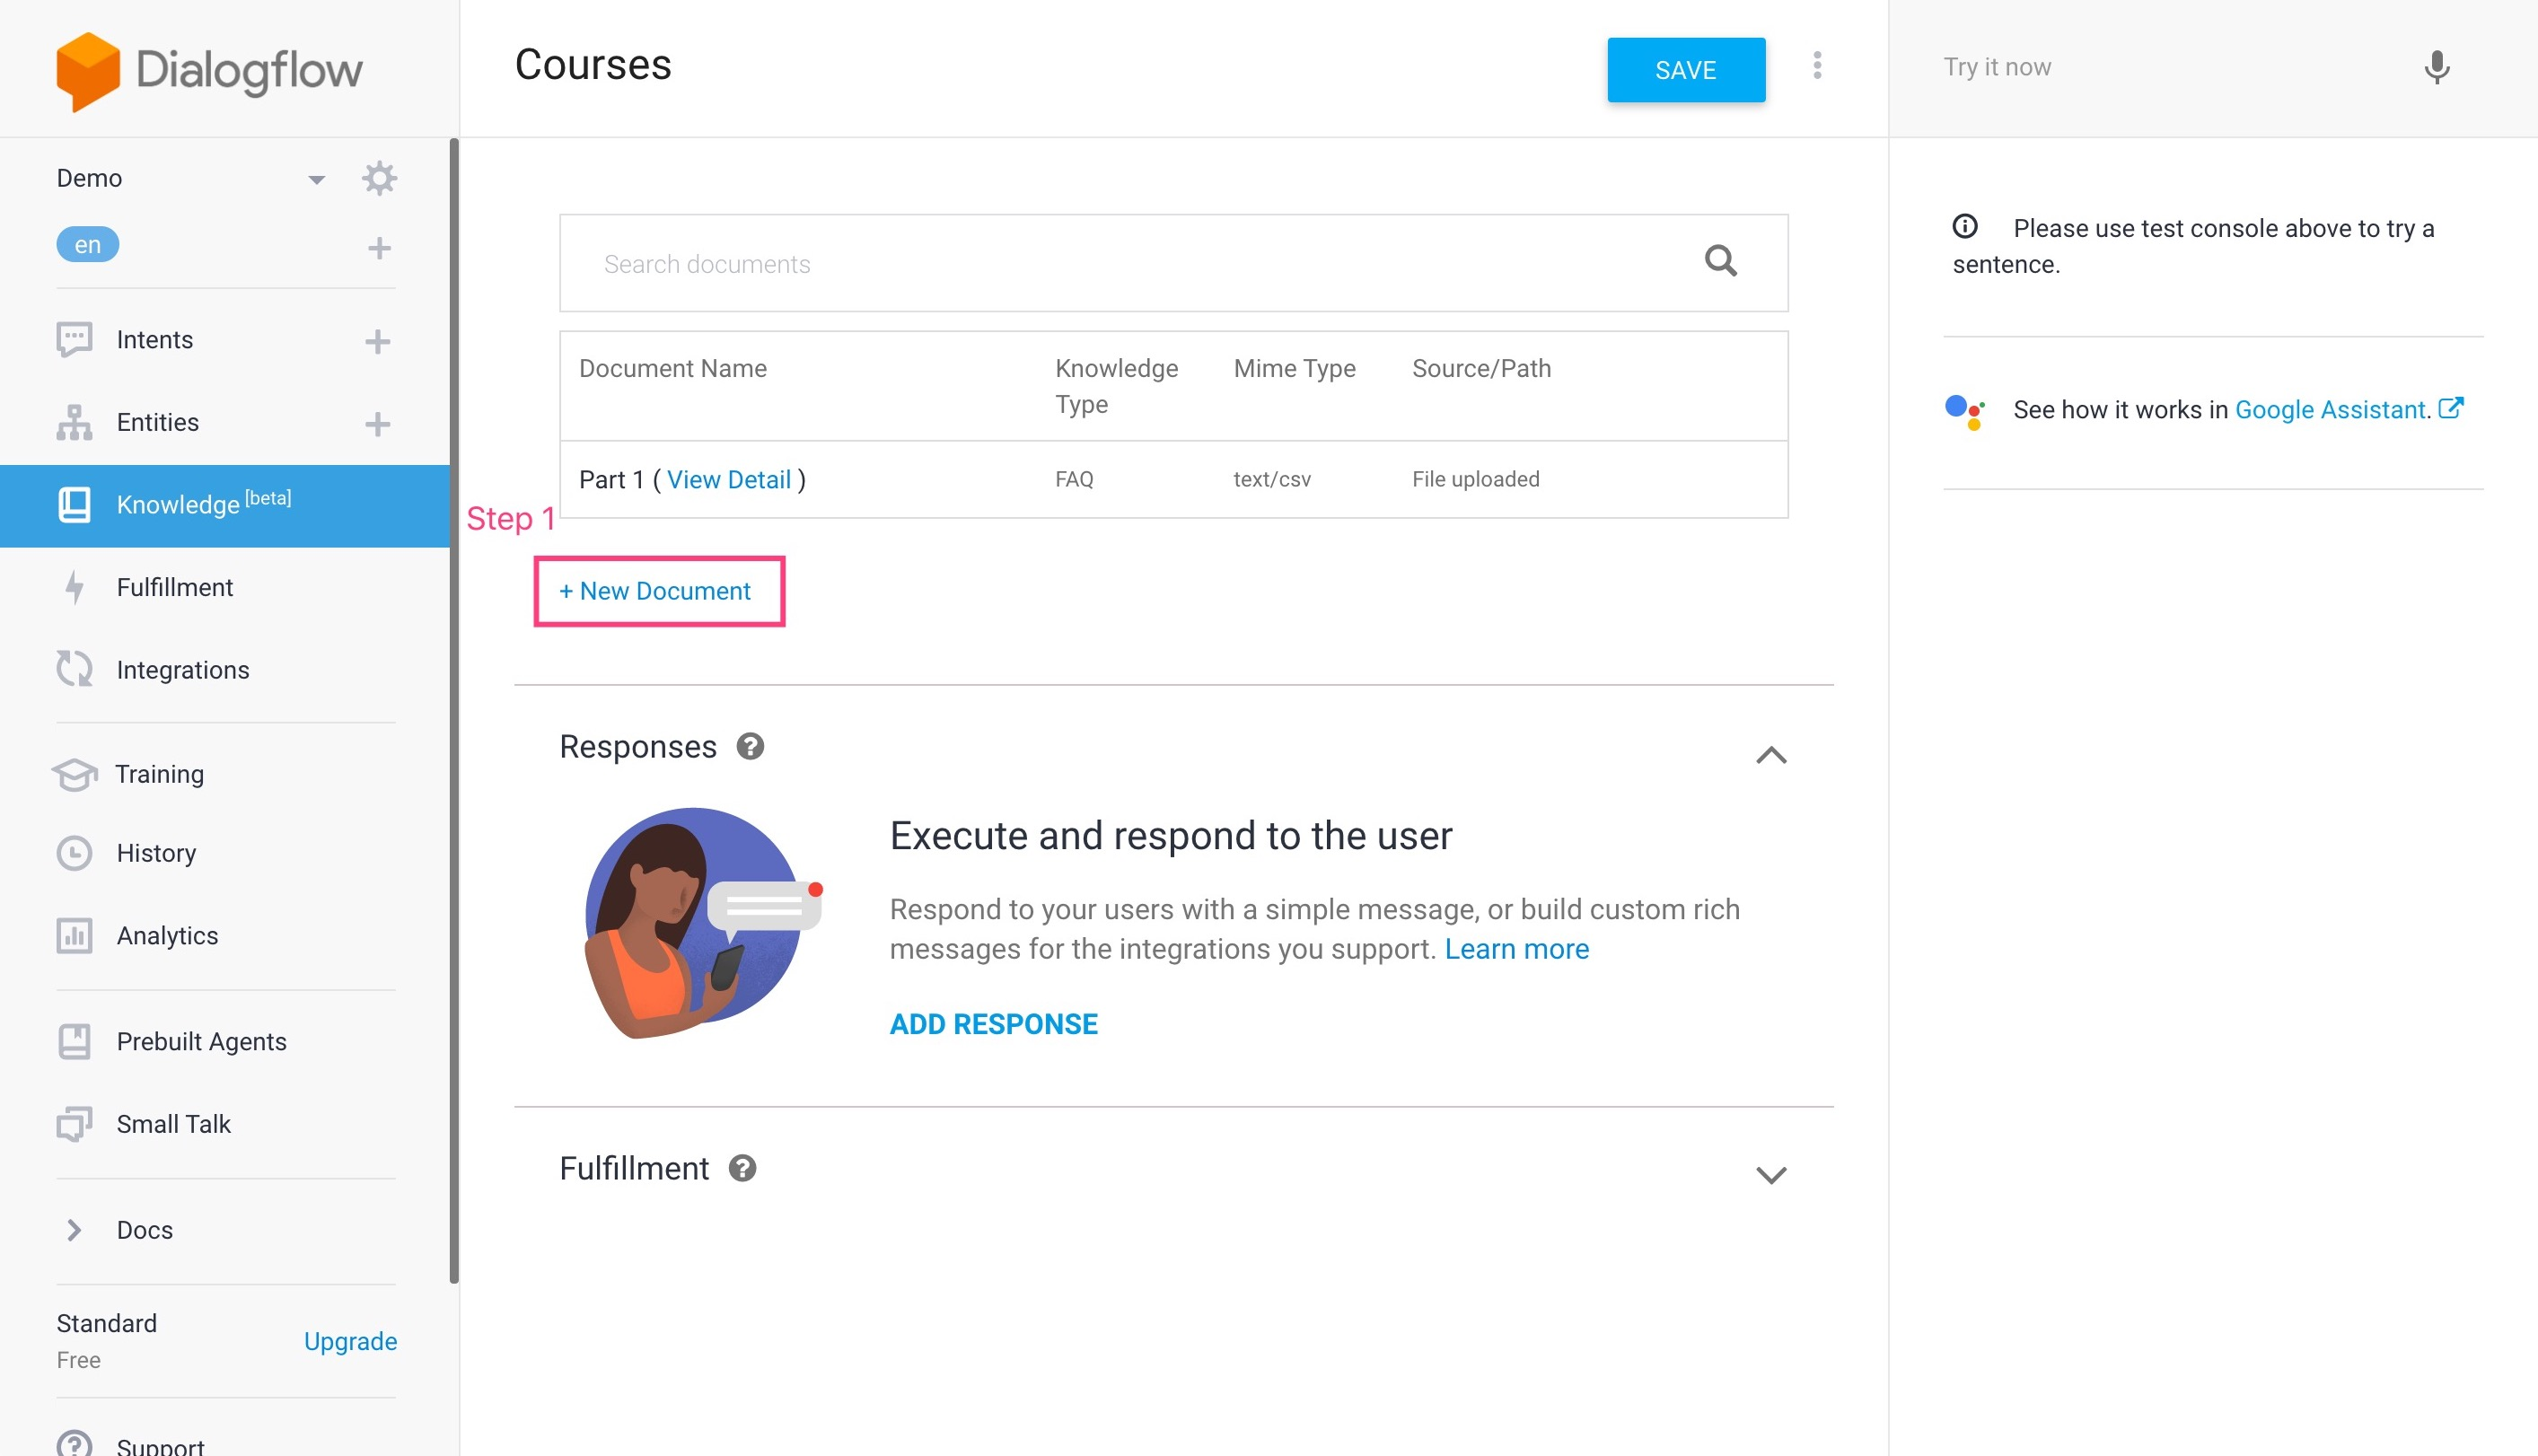
\includegraphics[width=\linewidth, frame]{img/manual_11.jpg}
	\end{figure}

	\item Input the fields as follows and upload “part2.csv”, then click “CREATE” button
	\nopagebreak
	\begin{figure}[H]
		\centering
		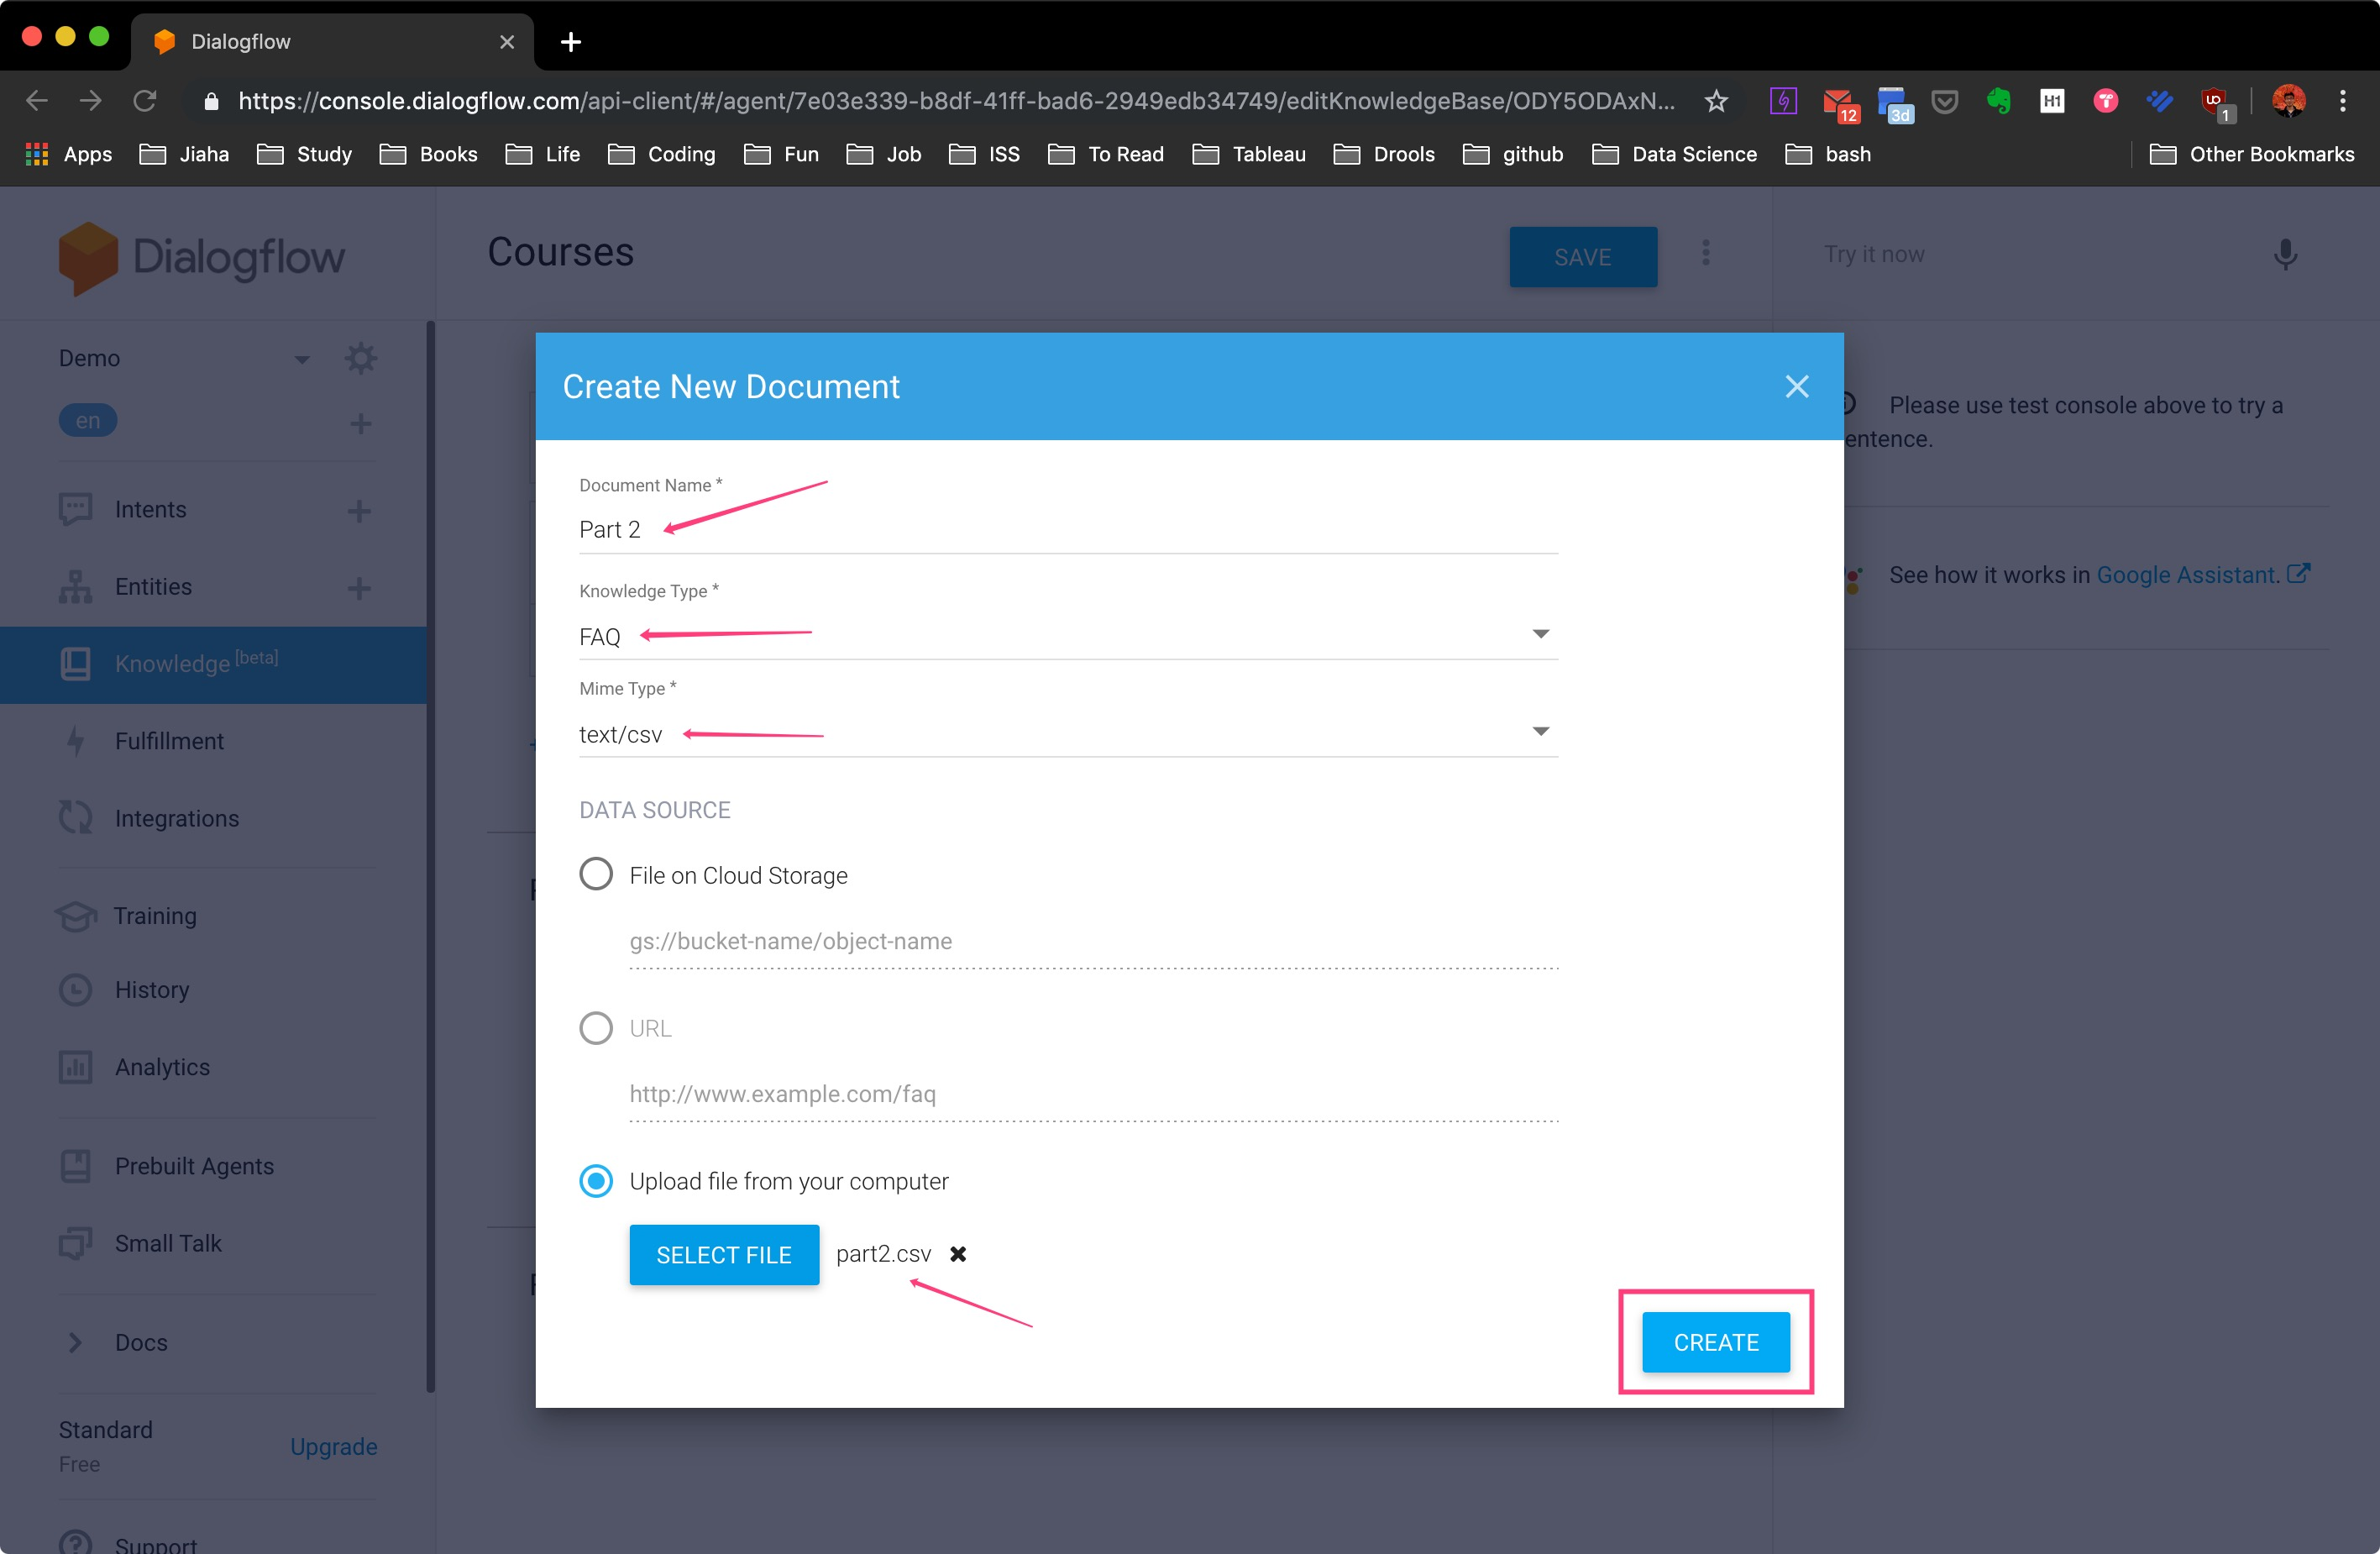
\includegraphics[width=\linewidth, frame]{img/manual_12.jpg}
	\end{figure}

	\item Click “ADD RESPONSE”
	\nopagebreak
	\begin{figure}[H]
		\centering
		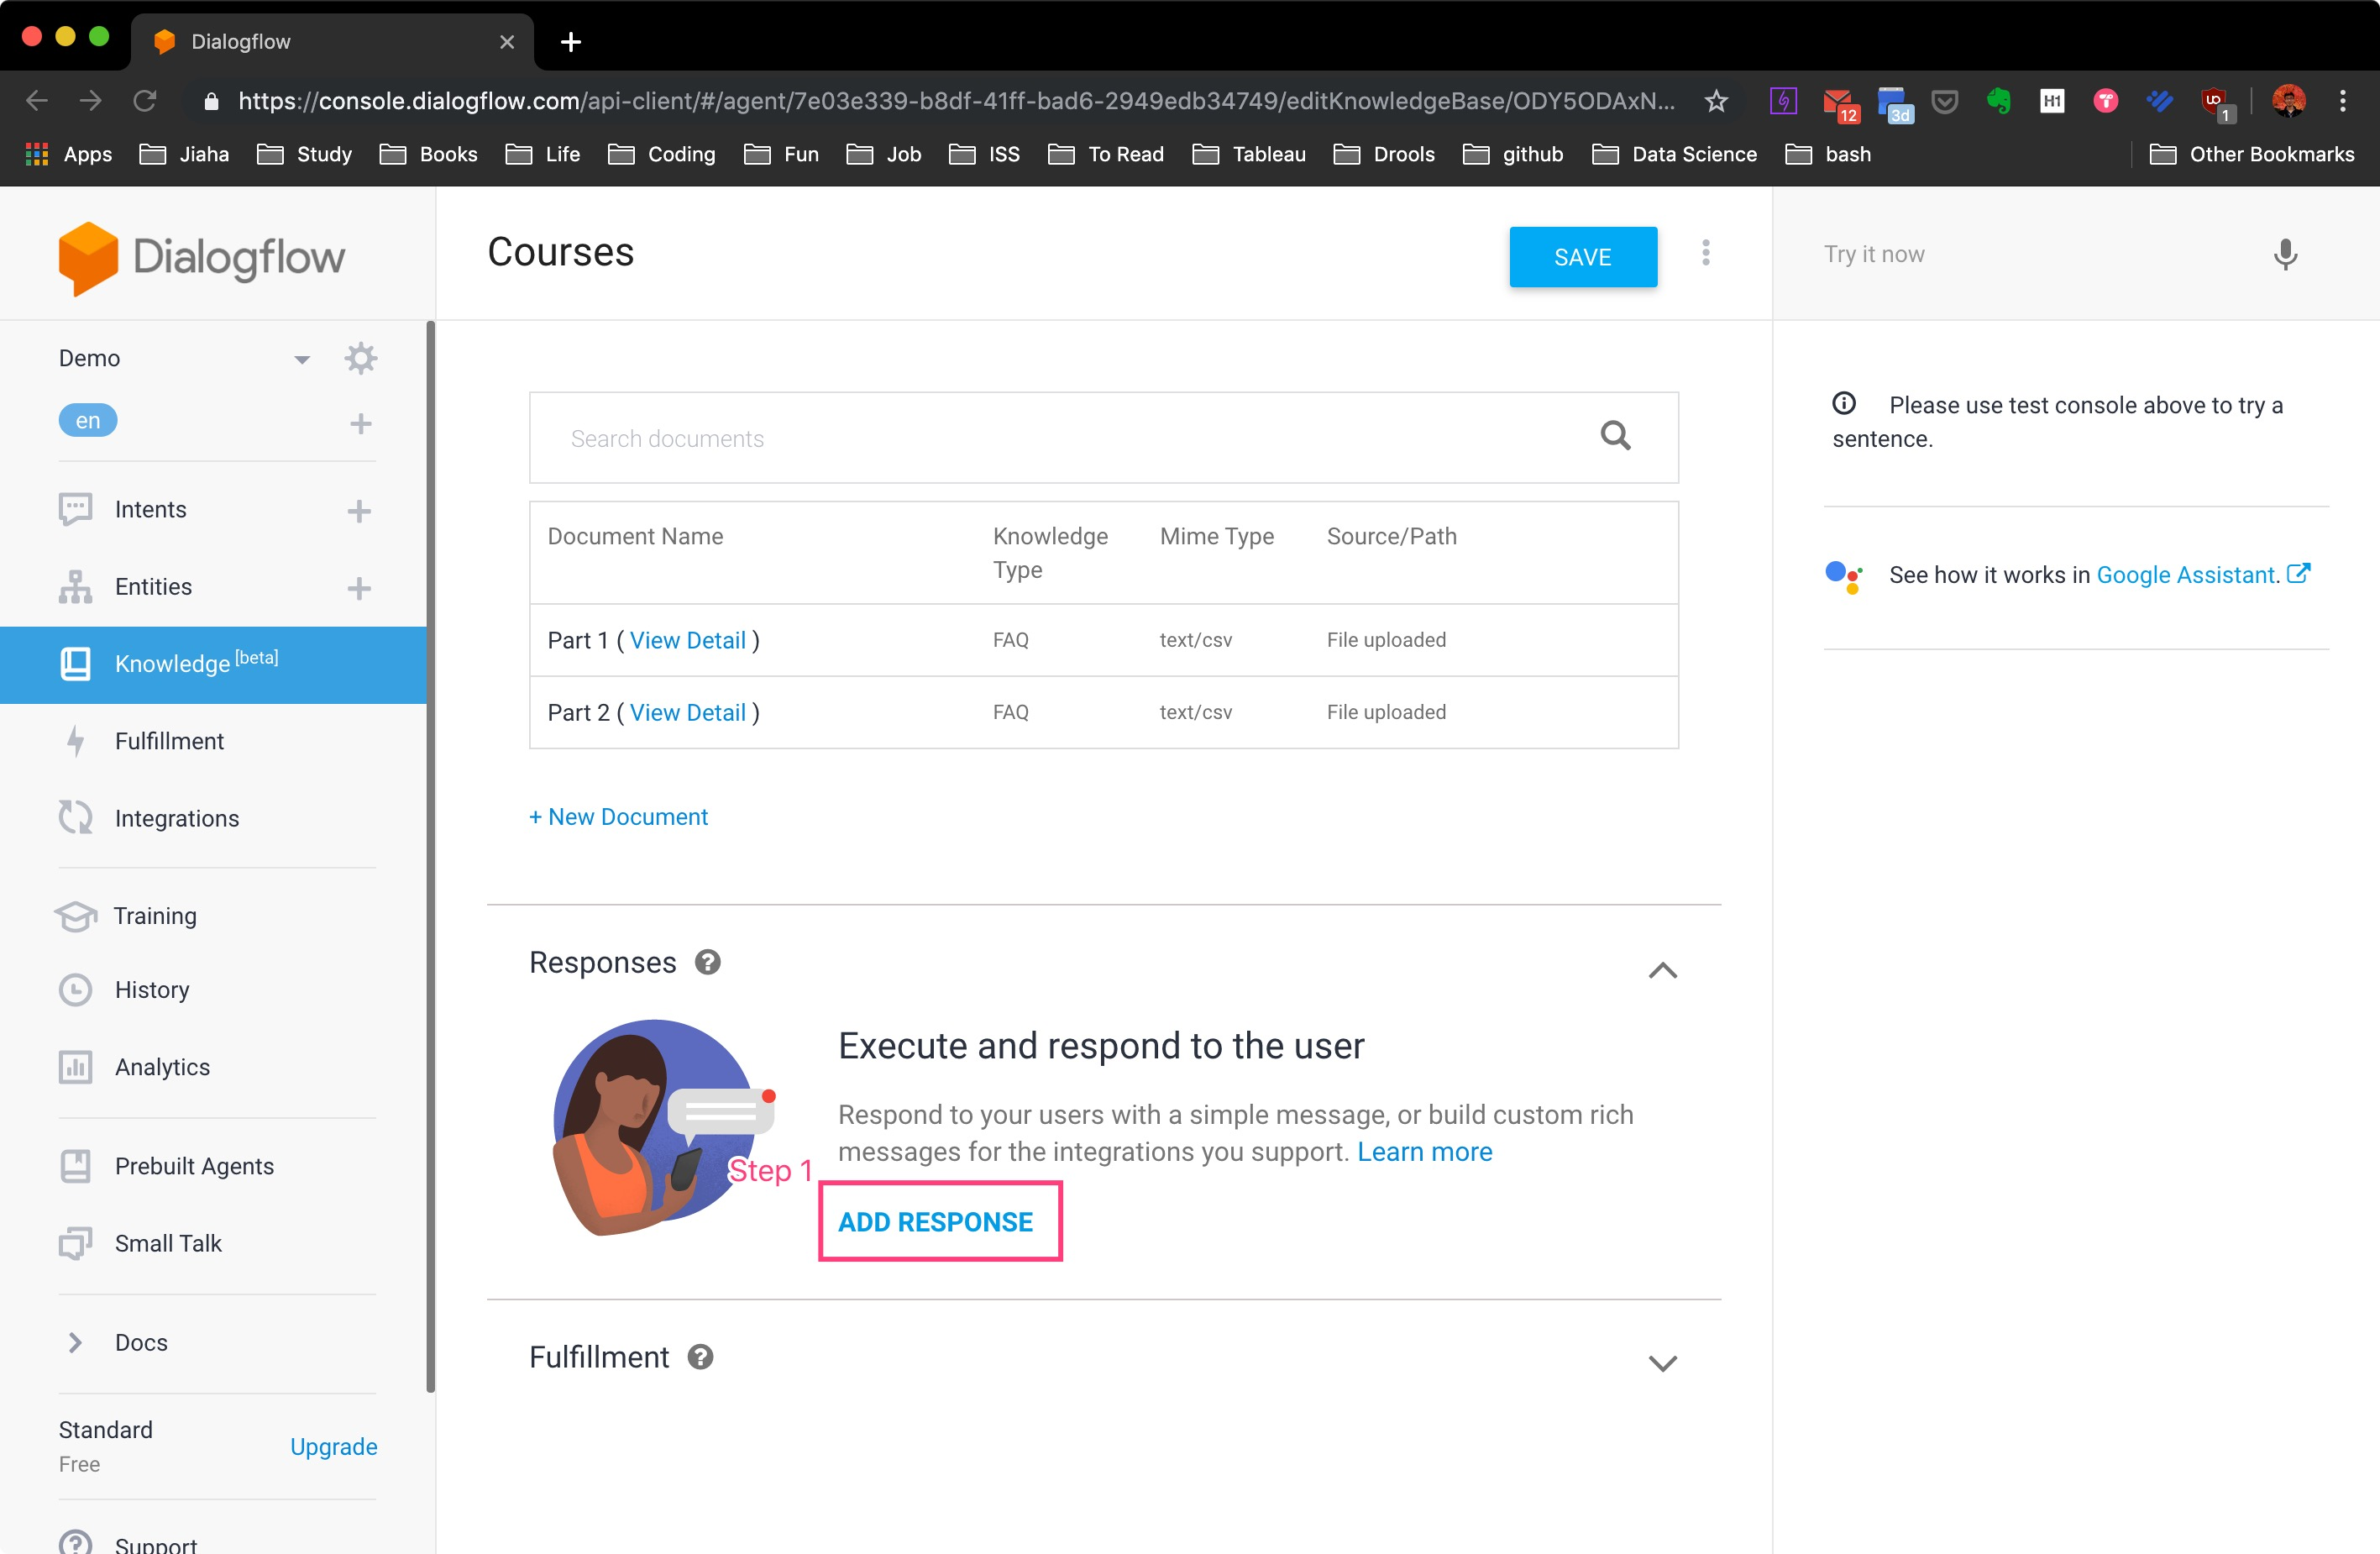
\includegraphics[width=\linewidth, frame]{img/manual_13.jpg}
	\end{figure}

	\item Click “SAVE” button
	\nopagebreak
	\begin{figure}[H]
		\centering
		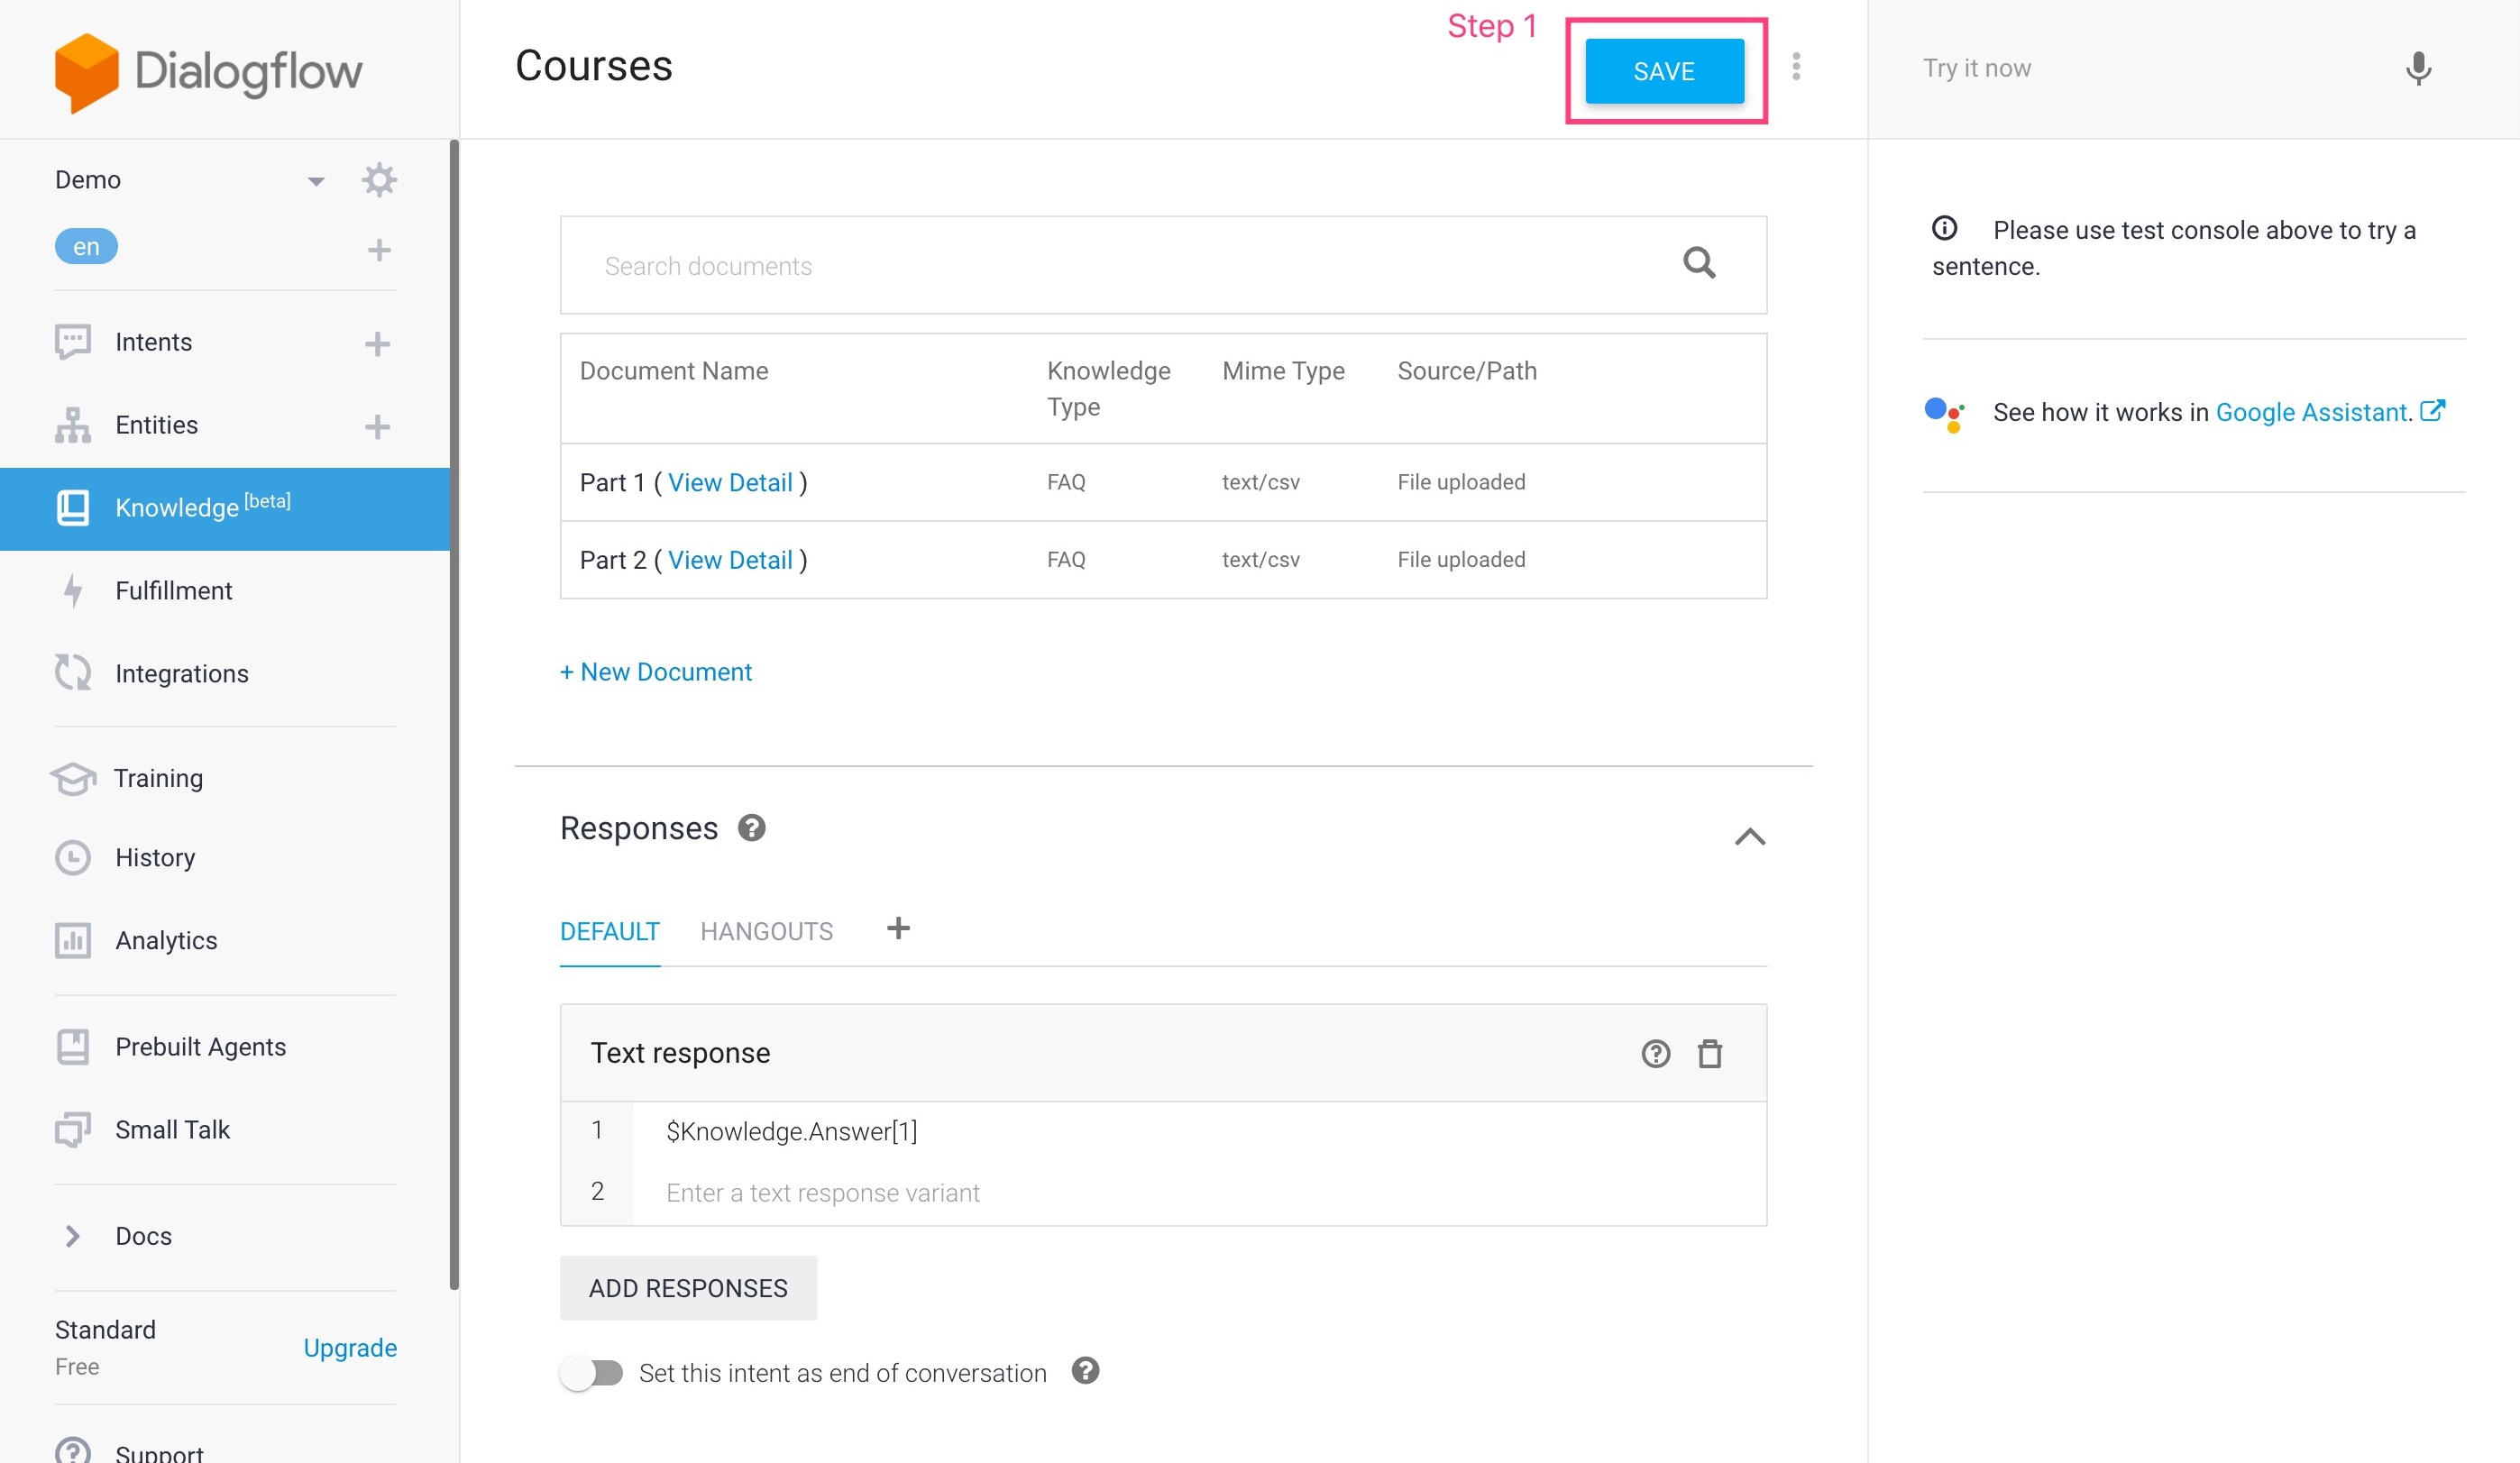
\includegraphics[width=\linewidth, frame]{img/manual_14.jpg}
	\end{figure}

\end{enumerate}
% section create_knowledge (end)

\section{Create Fulfilment} % (fold)
\label{sec:create_fulfilment}
	Click “Fulfillment” and enable “Inline Editor”, copy “IChat.js” and replace the content in “Index.js”. Then click “DEPLOY” button

	\begin{figure}[H]
		\centering
		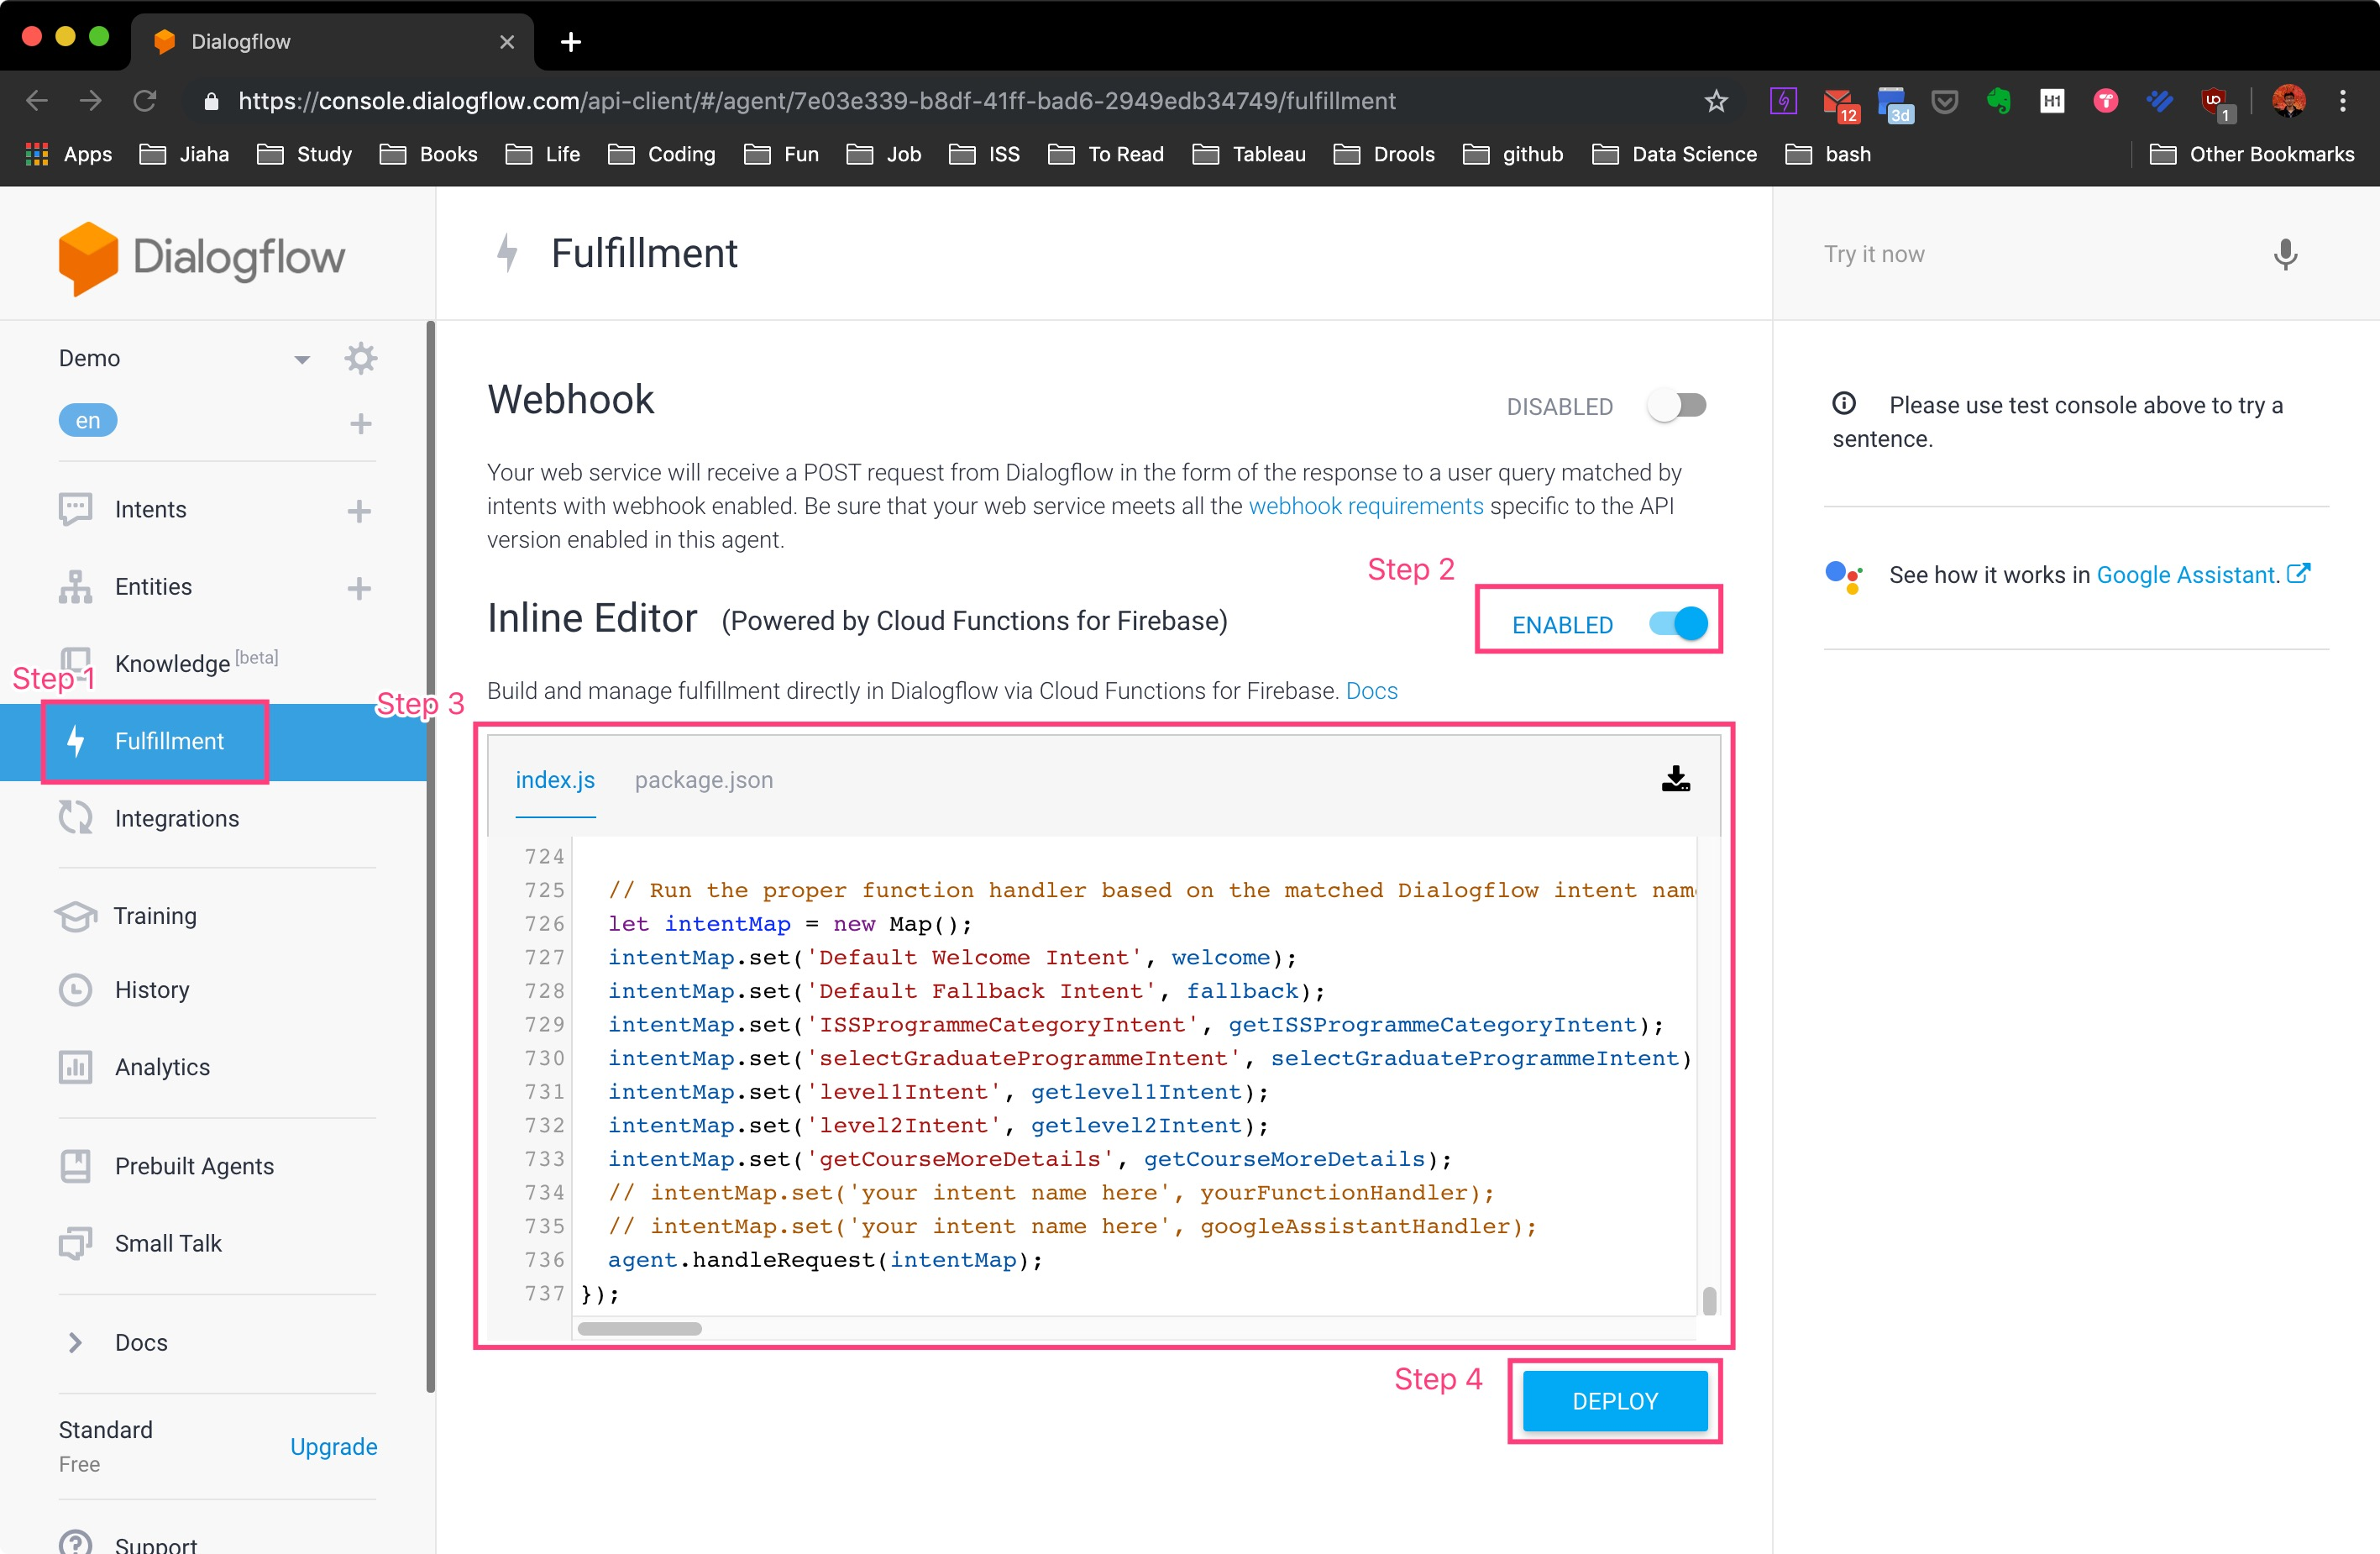
\includegraphics[width=\linewidth, frame]{img/manual_15.jpg}
	\end{figure}
% section create_fulfilment (end)

\section{Integration} % (fold)
\label{sec:integration}
	\begin{enumerate}
		\item Click “Integrations” and then enable “Slack”
		\nopagebreak
		\begin{figure}[H]
			\centering
			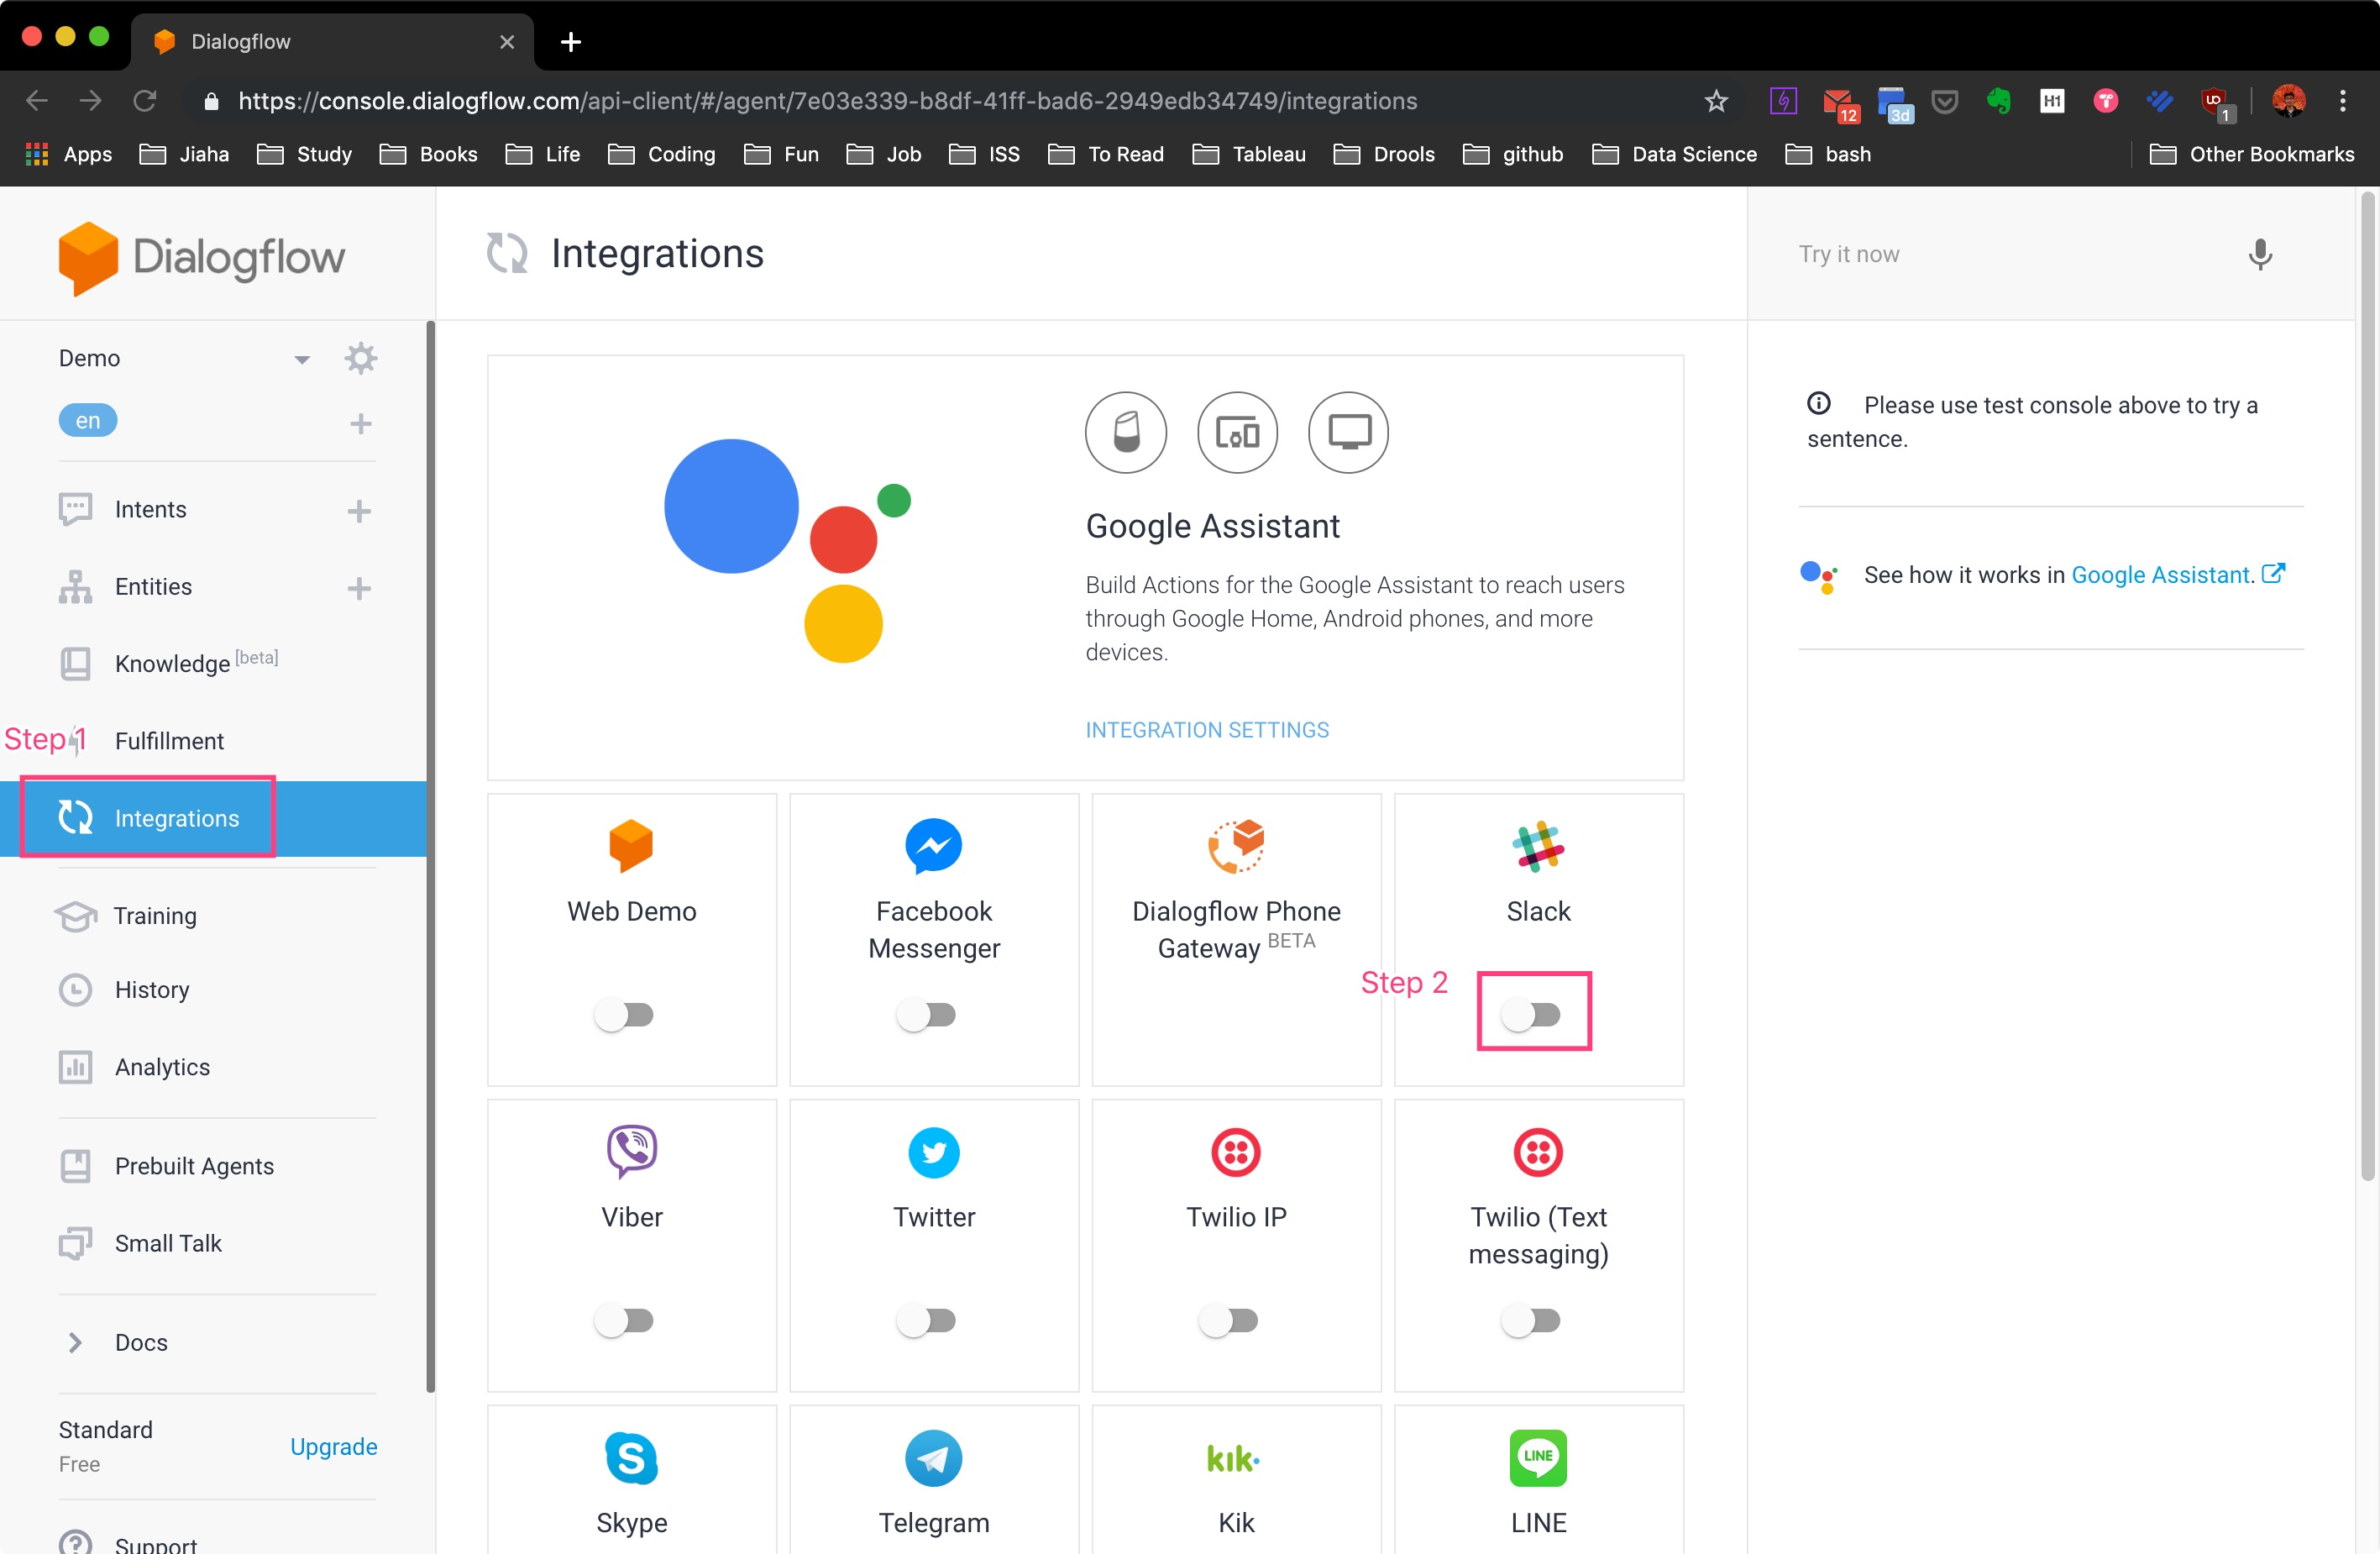
\includegraphics[width=\linewidth, frame]{img/manual_16.jpg}
		\end{figure}

		\item Follow the “Launch” to use, or click “TEST IN SLACK” with proper Slack set-up for testing

		\begin{figure}[H]
			\centering
			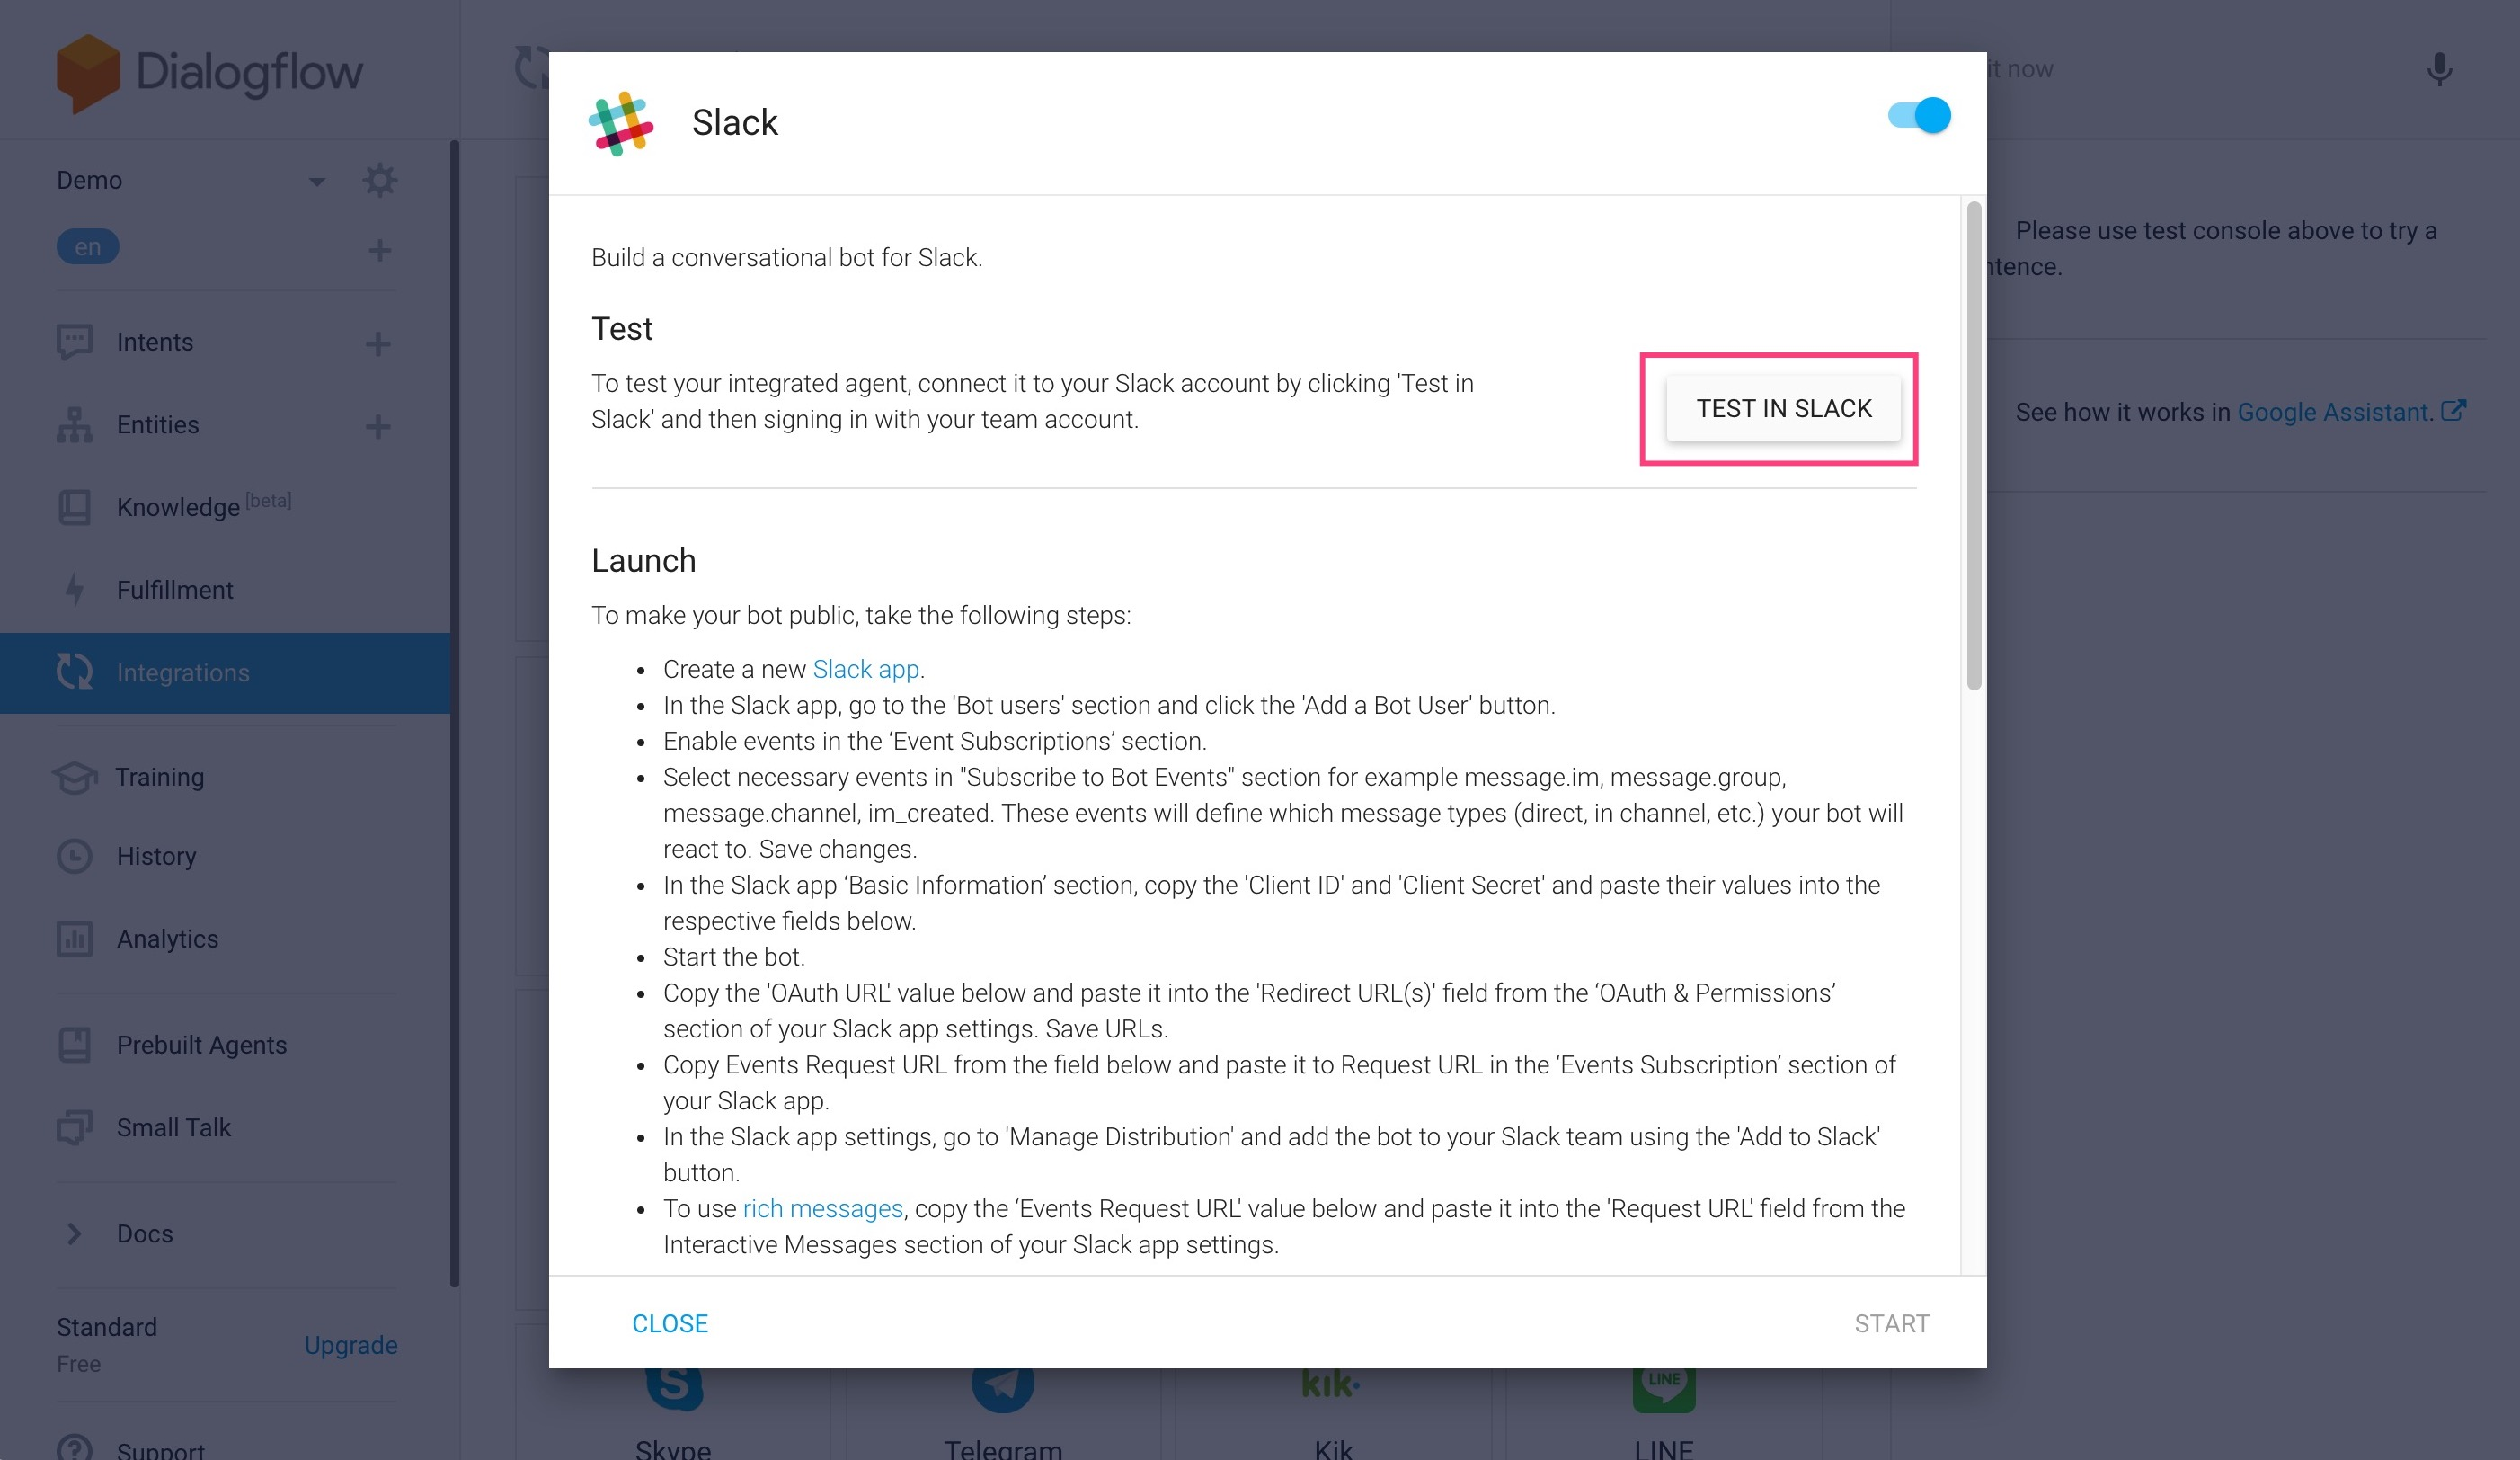
\includegraphics[width=\linewidth, frame]{img/manual_17.jpg}
		\end{figure}
	\end{enumerate}

% section integration (end)

\section{Test Demo} % (fold)
\label{sec:test}

	If Dialogflow is successfully integrated with Slack, you can say “hi” or other welcome words, and IChat will answer you enquiries.

	\begin{figure}[H]
		\centering
		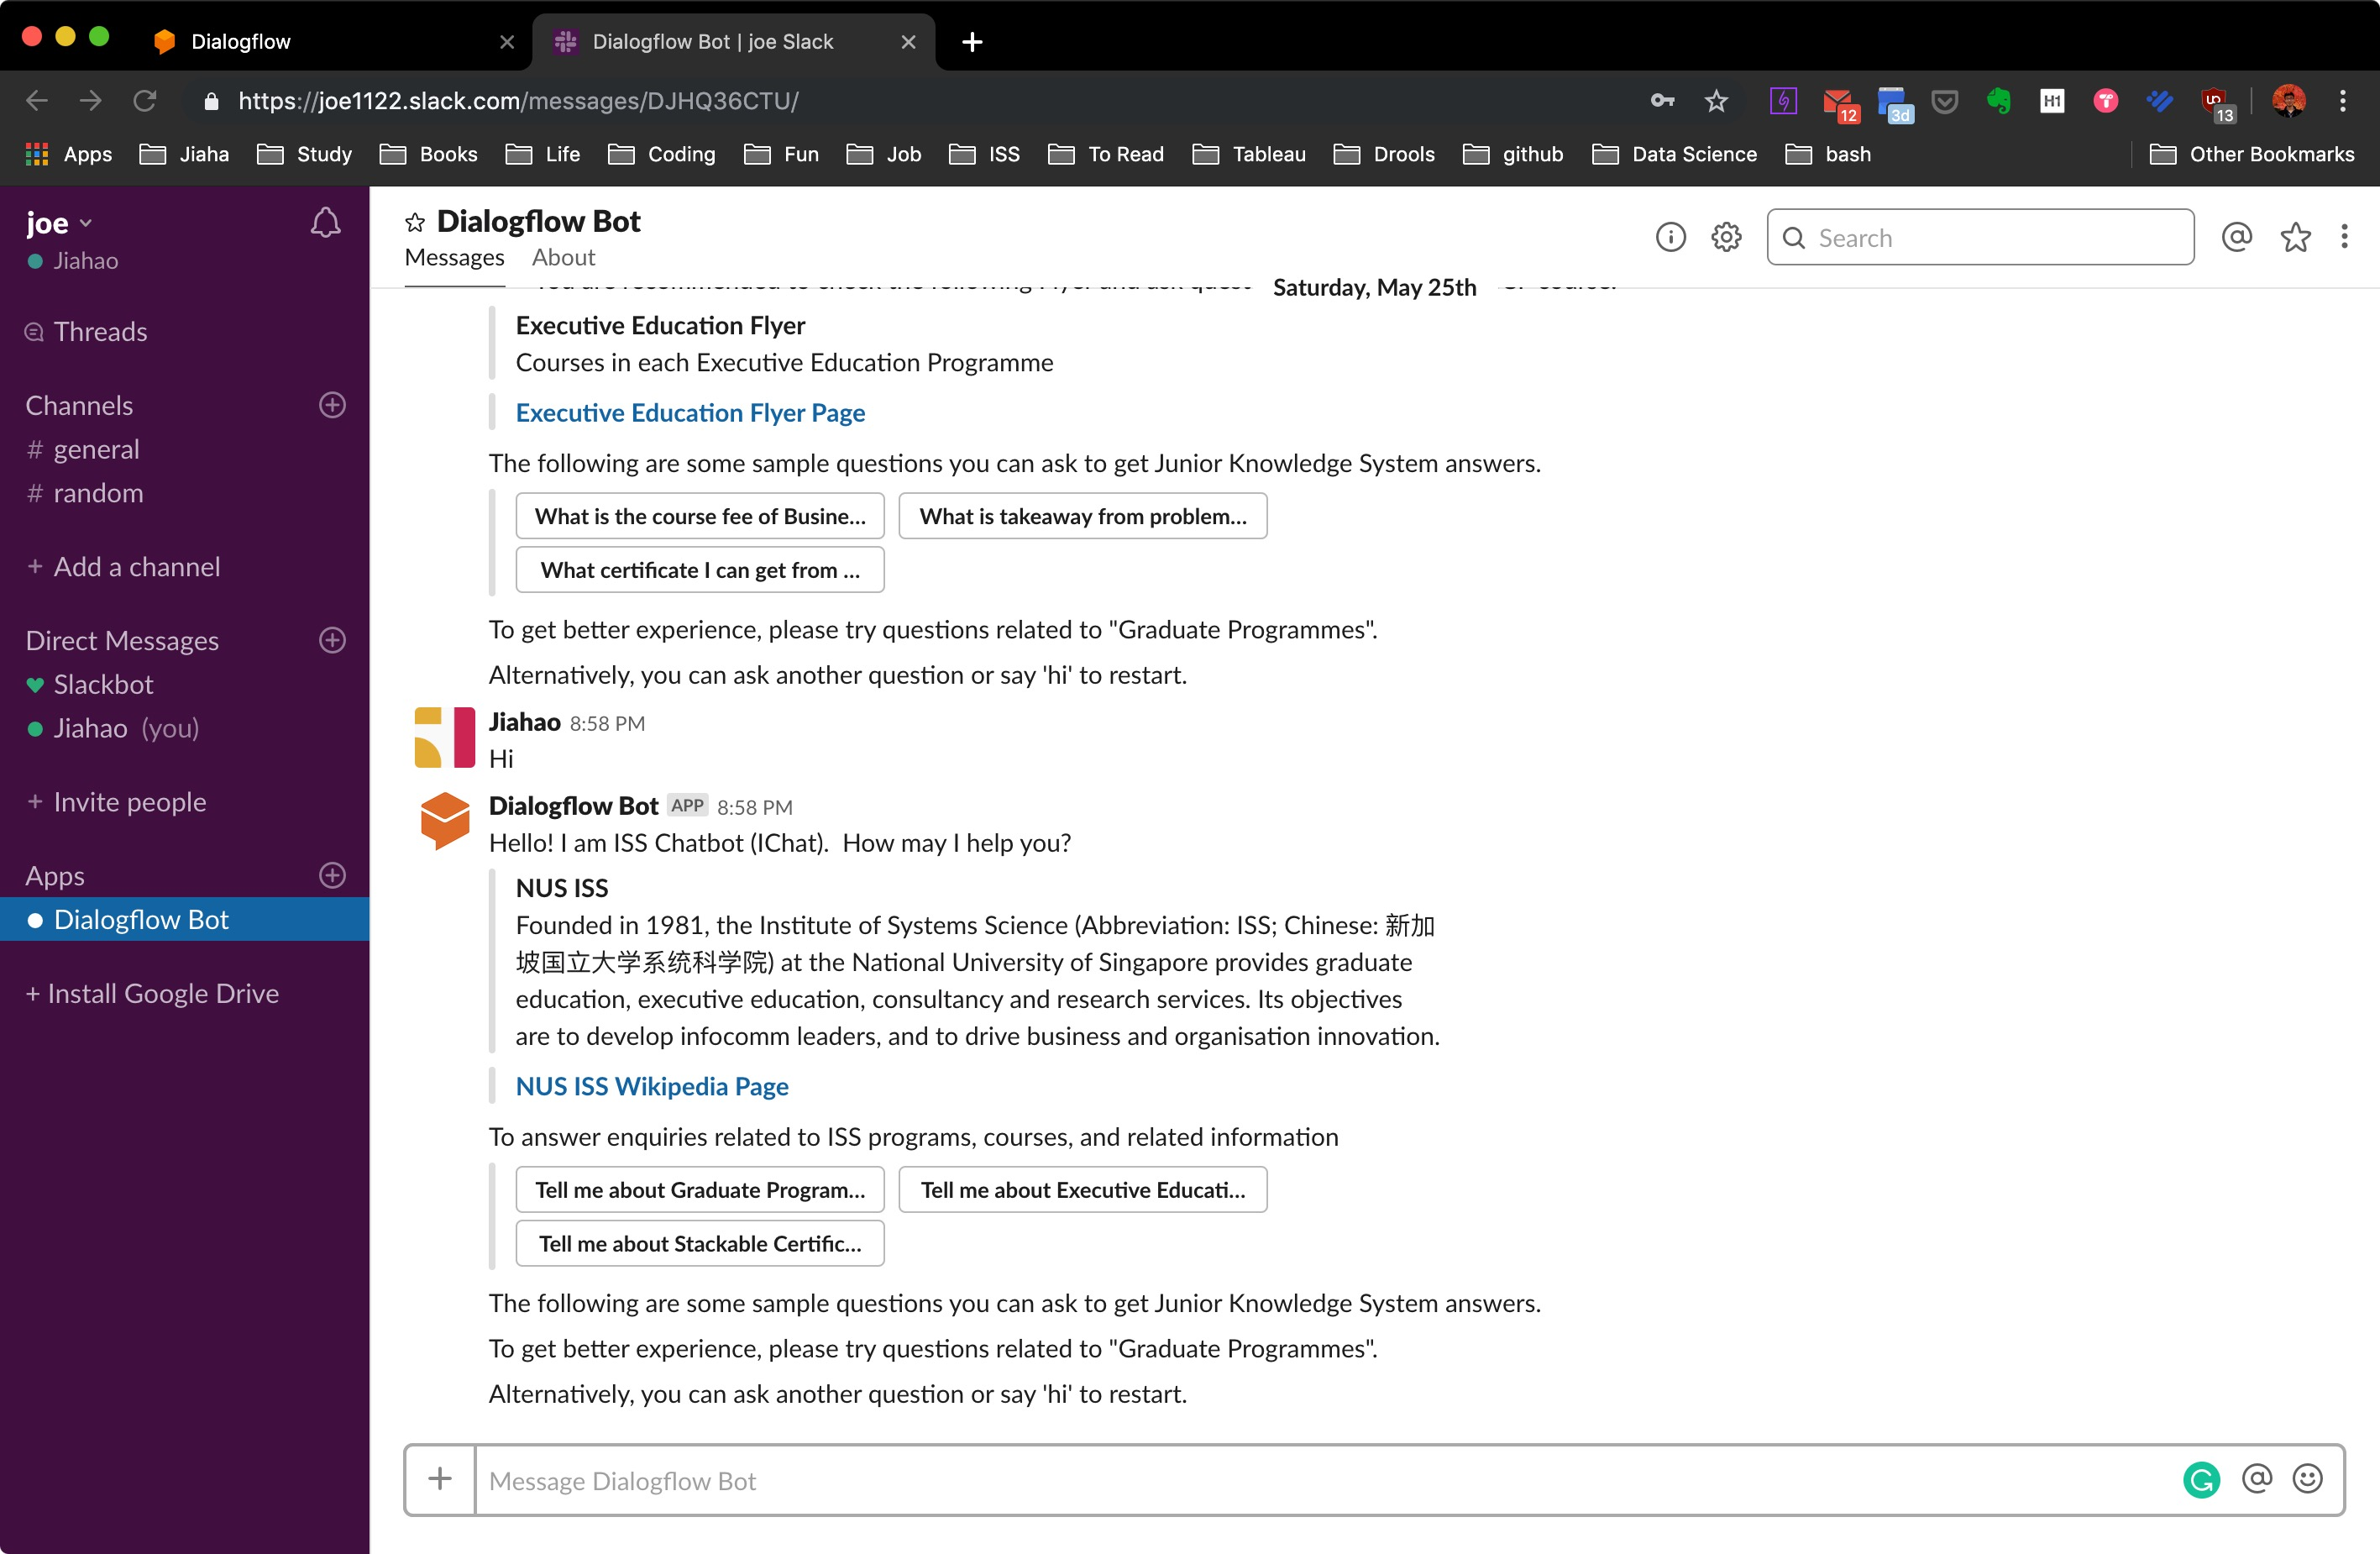
\includegraphics[width=\linewidth, frame]{img/manual_18.jpg}
	\end{figure}

	To easier test, the invite link is created for one of my demo.

	Here is the \href{https://join.slack.com/t/joe1122/shared_invite/enQtNjQxNTQ0MTY0Nzg1LTM3NDI3NGZjYWQzMjQ4YTJjMGIxZmQ4Y2VkMWYzNDAxOTQ0OTFlMmFjMzIzNDgyZjNkY2Q5YzQ2MjVlOTlmYWI}{\color{blue}{\underline{link}}}.

% section test (end)

\chapter{Test Result} % (fold)
\label{cha:test_result}

\begin{table}[h]
\centering
\resizebox{\textwidth}{!}{%
\begin{tabular}{|p{7cm}|p{5cm}|p{2cm}|p{2cm}|}
	\hline
	Can you give me an overview of Machine Reasoning? & Knowledge & 0.871 & \cellcolor[HTML]{9AFF99}Pass \\ \hline
	About Machine Reasoning & Knowledge & 0.671 & \cellcolor[HTML]{9AFF99}Pass \\ \hline
	What are the Machine Reasoning course pre-requsites? & Knowledge & 0.974 & \cellcolor[HTML]{9AFF99}Pass \\ \hline
	What are the Machine Reasoning course pre-requested knowledge? & Knowledge & 0.974 & \cellcolor[HTML]{9AFF99}Pass \\ \hline
	What are the Machine Reasoning course learning points? & Knowledge & 0.974 & \cellcolor[HTML]{9AFF99}Pass \\ \hline
	Learning result of Machine Reasoning & Knowledge & 0.587 & \cellcolor[HTML]{9AFF99}Pass \\ \hline
	What is the Machine Reasoning course key takeaway? & Knowledge & 0.974 & \cellcolor[HTML]{9AFF99}Pass \\ \hline
	Target Audience & Intent: Default Fallback Intent &  & \cellcolor[HTML]{FFCCC9}Fail \\ \hline
	Who should attend Machine Reasoning course? & Knowledge & 0.973 & \cellcolor[HTML]{9AFF99}Pass \\ \hline
	What will be covered in this Machine Reasoning course? & Knowledge & 0.976 & \cellcolor[HTML]{9AFF99}Pass \\ \hline
	What are the certs obtained from Machine Reasoning course? & Knowledge & 0.974 & \cellcolor[HTML]{9AFF99}Pass \\ \hline
	How much is Machine Reasoning? & Knowledge & 0.961 & \cellcolor[HTML]{9AFF99}Pass \\ \hline
	What are price for the Machine Reasoning? & Knowledge & 0.968 & \cellcolor[HTML]{9AFF99}Pass \\ \hline
	What are the Machine Reasoning course fees? & Knowledge & 0.974 & \cellcolor[HTML]{9AFF99}Pass \\ \hline
\end{tabular}%
}
\caption{FAQ Test}
\label{table:faq_test}
\end{table}

\begin{table}[h]
\centering
\resizebox{\textwidth}{!}{%
\begin{tabular}{|p{7cm}|p{5cm}|p{3cm}|}
	\hline
	\textbf{Test Question} & \textbf{Intent Returned} & \textbf{Final Test Case Result} \\ \hline
	Hi, tell me more about NUS ISS & Default Welcome Intent & \cellcolor[HTML]{9AFF99}Pass \\ \hline
	Graduate Programmes & ISSProgramCategoryIntent & \cellcolor[HTML]{9AFF99}Pass \\ \hline
	Overview of Master of Intelligence Systems & level1Intent & \cellcolor[HTML]{9AFF99}Pass \\ \hline
	Purpose & level2Intent & \cellcolor[HTML]{9AFF99}Pass \\ \hline
	Modules & level2Intent & \cellcolor[HTML]{9AFF99}Pass \\ \hline
	Price & level2Intent & \cellcolor[HTML]{9AFF99}Pass \\ \hline
	Application & level2Intent & \cellcolor[HTML]{9AFF99}Pass \\ \hline
	Career & level2Intent & \cellcolor[HTML]{9AFF99}Pass \\ \hline
	About Master of Intelligence Systems & level1Intent & \cellcolor[HTML]{9AFF99}Pass \\ \hline
	Learning Point & level2Intent & \cellcolor[HTML]{9AFF99}Pass \\ \hline
	Course & level2Intent & \cellcolor[HTML]{9AFF99}Pass \\ \hline
	Fees & level2Intent & \cellcolor[HTML]{9AFF99}Pass \\ \hline
	Application & level2Intent & \cellcolor[HTML]{9AFF99}Pass \\ \hline
	Furture Job & level2Intent & \cellcolor[HTML]{9AFF99}Pass \\ \hline
	Overview of Master of Intelligence Systems & level1Intent & \cellcolor[HTML]{9AFF99}Pass \\ \hline
	Purpose & level2Intent & \cellcolor[HTML]{9AFF99}Pass \\ \hline
	Courses & level2Intent & \cellcolor[HTML]{9AFF99}Pass \\ \hline
	School fee & level2Intent & \cellcolor[HTML]{9AFF99}Pass \\ \hline
	Admission & level2Intent & \cellcolor[HTML]{9AFF99}Pass \\ \hline
\end{tabular}%
}
\caption{Intent Test}
\label{table:intent_test}
\end{table}
% chapter test_result (end)

\chapter{Demo} % (fold)
\label{cha:demo}

	\section{Scenario 1} % (fold)
	\label{sec:scenario_1}
		A future student wants to check some information about \textbf{Master of Technology in Intelligent Systems}, which is under \textbf{Graduate Programme}. This student wants to know when the next intake time and how long will the programme last. In this scenario, the user only need to click suggestion button to get answers.

		\begin{figure}[H]
			\centering
			
\includegraphics[width=\linewidth, frame]{img/scenario_1.png}
		\end{figure}

		\begin{figure}[H]
			\centering
			
\includegraphics[width=\linewidth, frame]{img/scenario_2.png}
		\end{figure}

		\begin{figure}[H]
			\centering
			
\includegraphics[width=\linewidth, frame]{img/scenario_3.png}
		\end{figure}

		\begin{figure}[H]
			\centering
			
\includegraphics[width=\linewidth, frame]{img/scenario_4.png}
		\end{figure}

		\begin{figure}[H]
			\centering
			
\includegraphics[width=\linewidth, frame]{img/scenario_5.png}
		\end{figure}

		\begin{figure}[H]
			\centering
			
\includegraphics[width=\linewidth, frame]{img/scenario_6.png}
		\end{figure}
	% section scenario_1 (end)

	\section{Scenario 2} % (fold)
	\label{sec:scenario_2}
		An employee wants to learn more about \textbf{Machine Reasoning} course in \textbf{Executive Education Programmes}. The user needs to input questions related to the course in this scenario.

		\begin{figure}[H]
			\centering
			
\includegraphics[width=\linewidth, frame]{img/scenario_2_1.png}
		\end{figure}

		\begin{figure}[H]
			\centering
			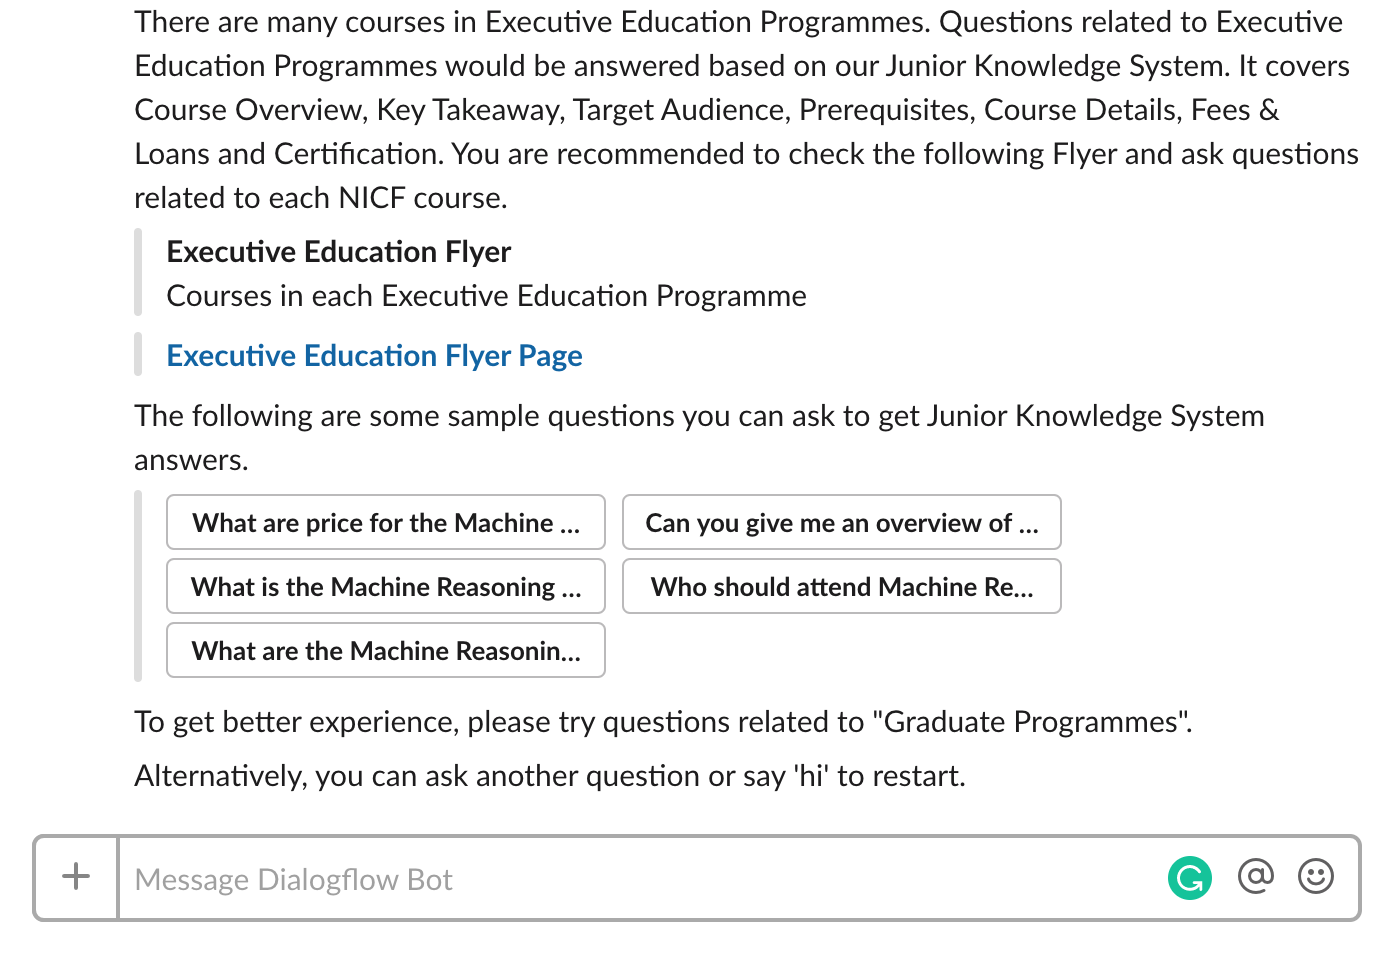
\includegraphics[width=\linewidth, frame]{img/scenario_2_2.png}
		\end{figure}

		\begin{figure}[H]
			\centering
			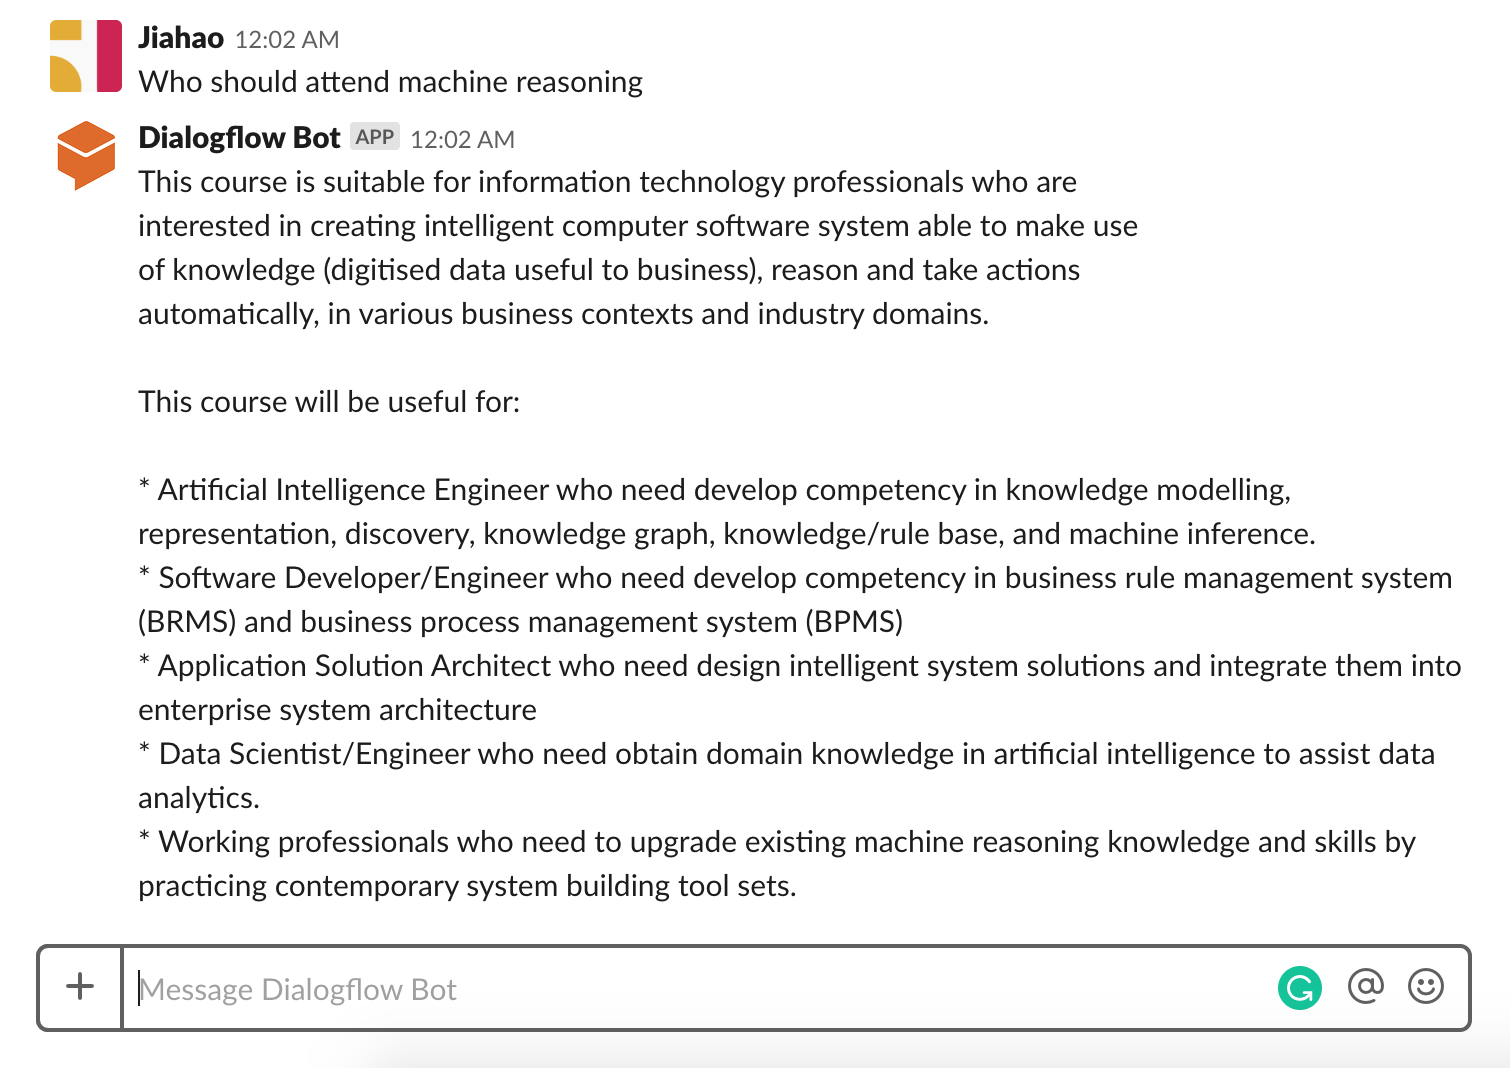
\includegraphics[width=\linewidth, frame]{img/scenario_2_3.png}
		\end{figure}

		\begin{figure}[H]
			\centering
			
\includegraphics[width=\linewidth, frame]{img/scenario_2_4.png}
		\end{figure}
	% section scenario_2 (end)
% chapter demo (end)



\chapter{Project Related Files} % (fold)
\label{sub:project_related_files}
	\textbf{Presentation Video:} \url{https://youtu.be/QOxnEkNSttI}

	\textbf{Intent and Test:} \url{https://github.com/yaaazhiii/IRS-CS-2019-04-27-IS1PT-GRP-IChat/blob/master/Miscellaneous/Intent%20and%20Test.xlsx}

% section project_related_files (end)


% section appendices (end)
\end{appendices}

\end{document}
